\documentclass[11pt]{article}

\usepackage[T1]{fontenc}
\usepackage{lmodern}
\usepackage{amsmath,amssymb,amsthm,mathtools}
\usepackage{mathrsfs}
\usepackage{graphicx,booktabs,array,enumitem}
\usepackage[margin=1in]{geometry}
\usepackage{microtype}
\usepackage{xcolor}
\usepackage[colorlinks=true,linkcolor=blue!45!black,citecolor=green!35!black,urlcolor=blue!55!black]{hyperref}
\hypersetup{pdftitle={Global Arthur Enhancements of Cuspidal Excursion Parameters},pdfauthor={OpenAI}}
\numberwithin{equation}{section}
\newtheorem{theorem}{Theorem}[section]
\newtheorem{proposition}[theorem]{Proposition}
\newtheorem{lemma}[theorem]{Lemma}
\newtheorem{corollary}[theorem]{Corollary}
\theoremstyle{definition}
\newtheorem{definition}[theorem]{Definition}
\newtheorem{notation}[theorem]{Notation}
\newtheorem{assumption}[theorem]{Assumption}
\theoremstyle{remark}
\newtheorem{remark}[theorem]{Remark}
\newcommand{\Q}{\mathbb Q}
\newcommand{\C}{\mathbb C}
\newcommand{\R}{\mathbb R}
\newcommand{\Z}{\mathbb Z}
\newcommand{\N}{\mathbb N}
\newcommand{\F}{\mathbb F}
\newcommand{\Gd}{\widehat G}
\newcommand{\g}{\mathfrak g}
\newcommand{\cO}{\mathcal O}
\newcommand{\cN}{\mathcal N}
\newcommand{\Fr}{\operatorname{Fr}}
\newcommand{\Frob}{\operatorname{Frob}}
\newcommand{\Ad}{\operatorname{Ad}}
\newcommand{\ad}{\operatorname{ad}}
\newcommand{\Lie}{\operatorname{Lie}}
\newcommand{\Hom}{\operatorname{Hom}}
\newcommand{\RHom}{\operatorname{RHom}}
\newcommand{\Map}{\operatorname{Map}}
\newcommand{\Ext}{\operatorname{Ext}}
\newcommand{\End}{\operatorname{End}}
\newcommand{\Rep}{\operatorname{Rep}}
\newcommand{\Perf}{\operatorname{Perf}}
\newcommand{\Coh}{\operatorname{Coh}}
\newcommand{\Ind}{\operatorname{Ind}}
\newcommand{\QCoh}{\operatorname{QCoh}}
\newcommand{\Spec}{\operatorname{Spec}}
\newcommand{\Sym}{\operatorname{Sym}}
\newcommand{\SL}{\operatorname{SL}}
\newcommand{\GL}{\operatorname{GL}}
\newcommand{\Sat}{\operatorname{Sat}}
\newcommand{\Tr}{\operatorname{Tr}}
\newcommand{\id}{\operatorname{id}}
\newcommand{\fib}{\operatorname{fib}}
\newcommand{\supp}{\operatorname{supp}}
\newcommand{\rk}{\operatorname{rk}}
\newcommand{\pt}{\operatorname{pt}}
\newcommand{\articleid}[1]{\begingroup\ttfamily\small\def\-{-\allowbreak}#1\endgroup}
\setlength{\emergencystretch}{2em}

\title{Global Arthur Enhancements\\of Cuspidal Excursion Parameters}
\author{OpenAI}
\date{October 5, 2026}
\begin{document}
\maketitle
\begin{abstract}
Under the finite-level Ramanujan--Arthur decomposition stated in
Theorem~\ref{thm:parent}, we construct a global Arthur enhancement for
every occurring cuspidal excursion parameter at a specified full finite
level for a split connected semisimple group over a global function field.
A single algebraic $\mathrm{SL}_2$ and a commuting Weil centralizer map
recover the given parameter by diagonal specialization on the entire Weil
group, including inertia. The result does not assert ellipticity,
Arthur-packet classification, or a multiplicity formula.
\end{abstract}
\tableofcontents

\section{Introduction}\label{sec:introduction}

An Arthur parameter separates two kinds of information in an automorphic
parameter: a part of weight zero and an algebraic $\SL_2$ that accounts for
its nonzero weights.  Over a global function field, the excursion construction
attaches a semisimple Galois parameter to cuspidal automorphic functions.
The question considered here is whether its weights come from one
$\SL_2$ commuting with its remaining global monodromy.  A decomposition
of the Frobenius conjugacy class at each place does not supply such a
commuting pair.  The pair must recover a fixed excursion parameter on
the entire Weil group.

\subsection{Excursion parameters and the statement}

Let $X$ be a smooth projective geometrically connected curve over
$\F_q$, let $F=\F_q(X)$, and let $G/\F_q$ be split, connected and
semisimple.  Fix an effective $\F_q$-defined divisor $D$, with arbitrary
multiplicities, and set $U=X\setminus\supp(D)$.  Write $\mathbb A_F$
for the adeles and $\mathcal O_{\mathbb A}$ for their integral subring.
The full level subgroup is
\[
 K_D=\ker\bigl(G(\mathcal O_{\mathbb A})\longrightarrow
                         G(\mathcal O_D)\bigr).
\]
For $D=0$ it is $G(\mathcal O_{\mathbb A})$.

Fix a prime $\ell\ne\operatorname{char}(\F_q)$, put
$k=\overline{\Q}_\ell$, and choose an embedding
$j:\overline{\Q}\hookrightarrow k$.  Let $L=\Gd$ be the split
Langlands dual group, equipped with its split rational form.  Let
$C_D$ be the $k$-space of compactly supported functions on
$G(F)\backslash G(\mathbb A_F)/K_D$ whose constant terms along all
proper $F$-parabolic subgroups vanish.  Thus, if $N$ is the unipotent
radical of such a subgroup, the condition is
\[
 \int_{N(F)\backslash N(\mathbb A_F)}f(ng)\,dn=0
 \qquad(g\in G(\mathbb A_F)).
\]
It is independent of the nonzero normalization of the Haar measure.
The space $C_D$ is finite dimensional.

Let $\mathcal B_D$ be the commutative image of the excursion operators
on $C_D$.  An \emph{occurring excursion character} is a character
$\nu:\mathcal B_D\to k$ with nonzero simultaneous generalized
eigenspace.  Its parameter is a conjugacy class of continuous
homomorphisms
\[
 \sigma_\nu:\pi_1(U)\longrightarrow L(k)
\]
defined over a finite extension of $\Q_\ell$, with reductive Zariski
closure.  The parameter theorem characterizes it by all excursion
evaluations: for every finite set $I$, regular function $h$ on
$L\backslash L^I/L$, and tuple $(\gamma_i)\in\pi_1(U)^I$,
\begin{equation}\label{intro:excursion}
 \nu(S_{I,h,(\gamma_i)})
       =h\bigl((\sigma_\nu(\gamma_i))_{i\in I}\bigr).
\end{equation}
Here the quotient denotes simultaneous left and right invariance.
This is the excursion parameterization, with its full tuple data
\cite[Theorems~0.1 and~11.11]{Hist:VLafforgue}.

Let $\Gamma=W_U$ be the inverse image of $\Z$ under
$\pi_1(U)\to\operatorname{Gal}(\overline{\F}_q/\F_q)=\widehat\Z$,
with its Weil topology.  We use the Frobenius and normalized Satake
conventions of~\cite{Parent}; in particular
\[
 \deg(\Frob_x)=d_x=[k(x):\F_q],\qquad q_x=q^{d_x}.
\]
Fix $a=j(\sqrt q)$ once and for all.  A Frobenius lift and a path to
the base point are chosen when an element, rather than a conjugacy
class, is needed.

The finite-level Ramanujan--Arthur decomposition is our spectral input.
We state precisely the consequence used below.

\begin{theorem}[Finite-level Ramanujan--Arthur decomposition
  {\cite[Theorem~1.1]{Parent}}]\label{thm:parent}
For every occurring excursion character $\nu$, there is a unique
nilpotent $L$-orbit $\mathcal O_\nu\subset\Lie L$ such that, at every
closed point $x\in U$, the semisimple class of
$\sigma_\nu(\Frob_x)$ has the form
\begin{equation}\label{intro:local-arthur}
 \left[
  \phi_{\mathcal O_\nu}
      \begin{pmatrix}a^{d_x}&0\\0&a^{-d_x}\end{pmatrix}c_x
 \right].
\end{equation}
Here $\phi_{\mathcal O_\nu}:\SL_2\to L$ is a
Jacobson--Morozov homomorphism for $\mathcal O_\nu$ and $c_x$ is
semisimple, centralizes its image, and is algebraic and conjugate
into a compact subgroup at every complex embedding.  The same orbit
occurs at every $x$.
\end{theorem}

The theorem is a statement about good-place semisimple classes.
We use it at that scope.  The choices of $c_x$ in
\eqref{intro:local-arthur} are not required to arise from a
homomorphism.  Our result supplies the global homomorphism and
retains the specified character $\nu$.

\begin{theorem}[Global Arthur enhancement]\label{thm:main}
Assume Theorem~\ref{thm:parent}.  For every $X,G,D,\ell,j$ and every
occurring excursion character $\nu$ as above, there are an algebraic
homomorphism
\[
 \phi_\nu:\SL_{2,k}\longrightarrow L
\]
and a continuous homomorphism
\[
 \tau_\nu:\Gamma\longrightarrow
                   Z_L\bigl(\phi_\nu(\SL_2)\bigr)(k),
\]
both defined over a finite extension of $\Q_\ell$, with the following
properties.
\begin{enumerate}[label=\textup{(\roman*)}]
 \item The differential of $\phi_\nu$ sends
       $\begin{psmallmatrix}0&1\\0&0\end{psmallmatrix}$ to
       $\mathcal O_\nu$.
 \item The Zariski closure of $\tau_\nu(\Gamma)$ is reductive.
       For every finite-dimensional algebraic representation $r$ of
       the split rational form of $L$ and every closed point $x\in U$,
       each eigenvalue of $r(\tau_\nu(\Frob_x))$ lies in
       $j(\overline\Q)$ and its inverse image under $j$ has absolute
       value one under every embedding $\overline\Q\hookrightarrow\C$.
 \item After one fixed $L(k)$-conjugation of $\sigma_\nu$,
       \begin{equation}\label{intro:global-specialization}
       \sigma_\nu(w)=\tau_\nu(w)\,
           \phi_\nu\begin{pmatrix}a^{\deg(w)}&0\\0&a^{-\deg(w)}\end{pmatrix}
       \qquad(w\in\Gamma).
       \end{equation}
\end{enumerate}
The centralizer is the full algebraic centralizer; it may be
disconnected.
\end{theorem}

Equivalently,
$\Psi_\nu(w,h)=\tau_\nu(w)\phi_\nu(h)$ is a homomorphism
$\Gamma\times\SL_2\to L$ with the prescribed diagonal
specialization.  Equation~\eqref{intro:global-specialization} holds
on geometric monodromy and on the inertia groups at the points of
$D$, as well as on Frobenius elements.  The conclusion concerns the
original curve and level.


\subsection{Historical context and related work}

Arthur's conjectures explain the non-tempered part of the discrete
spectrum by supplementing a tempered parameter with an algebraic
$\mathrm{SL}_2$ whose image commutes with it.  This structure appeared
in his Maryland lectures, published in 1984, and was developed in his
subsequent formulation of unipotent automorphic representations
\cite[Sections~1.3 and~2.1]{history:Arthur1984}
\cite[Section~8]{history:Arthur1989}.
The diagonal specialization of this additional $\mathrm{SL}_2$
accounts for the prescribed powers of the residue-field cardinality
in the associated Langlands parameter.  The corresponding global
conjectures also concern packets and their multiplicities; the
existence of a commuting pair is one part of that larger structure.

Over function fields, Drinfeld's work for $\mathrm{GL}_2$ and
Laurent Lafforgue's work for $\mathrm{GL}_n$ realized the Langlands
correspondence in the cohomology of shtukas
\cite{history:Drinfeld1980,history:LLafforgue}.
Laurent Lafforgue's purity theorem for irreducible lisse sheaves with
finite-order determinant supplies the weight input used here
\cite[Theorem~VII.6]{history:LLafforgue}.
Vincent Lafforgue subsequently constructed excursion operators and
attached semisimple global parameters to cuspidal automorphic
functions for reductive groups at arbitrary finite level
\cite[Theorems~0.1 and~11.11]{Hist:VLafforgue}.
These operators retain invariants of tuples of Galois elements,
so the resulting parameter contains more information than its
individual unramified Frobenius classes.  His Arthur conjecture
\cite[Section~12.2.2 and Conjecture~12.7]{Hist:VLafforgue}
asks that each occurring parameter arise from an elliptic global
Arthur parameter.

In the everywhere unramified setting, Gaitsgory--Lafforgue--Raskin
formulate the Ramanujan--Arthur
decomposition by requiring the same nilpotent-orbit spectral type
at every unramified place
\cite[Section~3.4.3, Conjectures~3.4.5--3.4.6, and Remark~3.4.7]{history:GLR}.
They distinguish this condition from support on global Arthur
parameters, which is formulated separately in
\cite[Section~3.6]{history:GLR}.
The finite-level theorem of \cite[Theorem~1.1]{Parent}, recalled
in Theorem~\ref{thm:parent}, supplies the former condition for
arbitrary full level.  Passing from that condition to one commuting
pair requires compatibility with the complete excursion parameter,
rather than a separate choice of a triple at each closed point.

A global enhancement in the everywhere unramified setting has
already been announced by Raskin as part of joint work with
Gaitsgory and Lafforgue
\cite[Theorem~C]{history:RaskinAnnouncement}.
That announcement recovers the specified cuspidal excursion
parameter from a commuting $W_X\times\mathrm{SL}_2$ parameter
and asserts irreducibility of the latter, under the standing
characteristic hypotheses of its Section~1.1.1.
Theorem~\ref{thm:main} treats arbitrary full finite level under
the finite-level decomposition hypothesis.  Its conclusion is
the existence and purity of the commuting pair stated there;
the conclusion does not impose ellipticity or give a packet
multiplicity formula.

The local geometry in the proof combines several established
constructions.  Geometric Satake identifies spherical perverse
sheaves with representations of the dual group
\cite{history:MV}; the derived calculation of
Bezrukavnikov--Finkelberg adds the polynomial directions on its
Lie algebra \cite{history:BF}.
Gaitsgory's nearby-cycles construction produces central sheaves
in the affine flag category \cite{history:Gaitsgory}.
Bezrukavnikov's comparison of the constructible and coherent
realizations of the affine Hecke category
\cite{Enh:Bezrukavnikov} and the coherent trace theorem of
Ben-Zvi--Chen--Helm--Nadler \cite{Local:BZCHN} then provide the
local coherent models.  The comparisons developed below retain
Frobenius, central labels, and change of level simultaneously.
These compatibilities are needed to apply the local models at
several places to one global support module.

The global cohomological input comes from Xue's finiteness and
smoothness theorems for stacks of shtukas
\cite{Bounds:XueFiniteness,Bounds:XueSmoothness}.
They allow the excursion and partial-Frobenius formalism to be
used on the cohomology carrying the local tests.  The parahoric nearby-cycles
comparison of Salmon \cite[Theorem~5.2(1)]{Bounds:SalmonNearby}
relates those tests to fibers at distinct points.  The more general
restricted-coefficient comparison is developed by Eteve--Xue
\cite{Bounds:EteveXueNearby}.  The parahoric comparison, together
with the constituent purity theorem, brings the cohomological
weight bound into the simultaneous local calculation.


\subsection{The proof mechanism}

Put $A=L_{\mathrm{ad}}$ and $\g=\Lie L=\Lie A$.
We first attach to a nonzero $\nu$-eigenvector $f\in C_D$ a
finite-type affine scheme $\Spec R$.  A point of this scheme records a homomorphism
$b:\Gamma\to A(k)$ and an element $e\in\g$ satisfying
\begin{equation}\label{intro:scaling}
       \Ad(b(w))e=q^{\deg(w)}e\qquad(w\in\Gamma).
\end{equation}
The invariant evaluations of every tuple of $b$ are those of
$\sigma_{\nu,\mathrm{ad}}$.  The construction uses matrix entries
of partial Weil actions on regular Satake labels, together with a
degree-two operation.  It is this tuple information that eventually
recovers the chosen global parameter.

At suitably chosen good places $x$, choose a representative $t_x$
of the semisimple Frobenius class and consider the resonance space
\[
 E_{t_x}=\{e\in\g:\Ad(t_x)e=q_xe\}.
\]
The connected centralizer of $t_x$ has a unique open orbit, whose elements
belong to $\mathcal O_\nu$.  If a point of $\Spec R$ reaches this
open orbit at even one test place, the scaling relation yields a
global commuting pair.  Levi projection and the full tuple
identities give the required simultaneous conjugation; a norm
argument then proves weight zero.  Consequently, failure of
Theorem~\ref{thm:main} would force the image of $\Spec R$ into
the boundary at every test place.

The rest of the proof rules out this boundary condition.  At the $i$th
test place, a coherent comparison identifies the hyperspecial object
with the structure sheaf $B_i=\cO_{Y_i}$ of an ordinary complete
intersection $Y_i$.  Let $P_i^{\mathrm{bad}}$ be the sum of the
derived direct images of structure sheaves from those local flag spaces whose
vector images miss the open orbit.  Their structure-sheaf units define
\[
 Q_i=\fib(B_i\longrightarrow P_i^{\mathrm{bad}}),\qquad
 q_i:Q_i\longrightarrow B_i.
\]
Every boundary point supplied by the global support lies under one
of these flag spaces.  On its derived residue-field fiber, evaluation at a flag
splits the unit map, so the fiber map $q_i$ is zero.

Shtuka smoothness, nearby cycles and constituent purity give one lower
cohomological bound, independent of the number of test places.  This
permits the local tests to act on the global support in ordinary
quasi-coherent complexes.  If every local image of $\Spec R$ lies in
the boundary, each $q_i$ therefore vanishes on every derived
residue-field fiber of this support.  A noetherian tensor argument gives
a finite product $q_\Pi=\boxtimes_{i=1}^nq_i$ for which $q_\Pi^*f=0$.

On the other hand, a simple quotient of the cuspidal Iwahori Hecke
module detects $f$ and is annihilated by the idempotents of all the
summands in $P_i^{\mathrm{bad}}$.  Applying shtuka cohomology to the
defining fiber diagrams for $Q_i$ shows that $f$ survives their
product: $q_\Pi^*f\ne0$.  This contradiction forces an open-orbit point
and completes the global enhancement.  Figure~\ref{fig:proof-architecture}
records the dependencies of these two conclusions.

\begin{figure}[p]
 \centering
 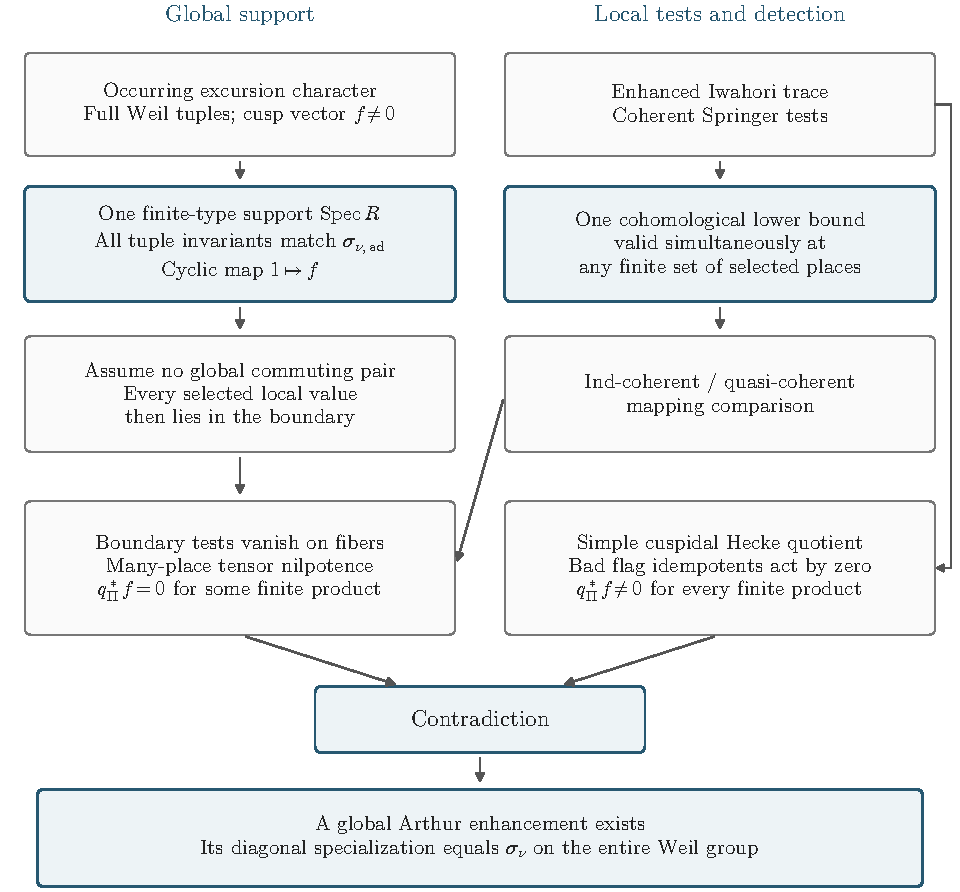
\includegraphics[width=\textwidth]{figures/proof-architecture.pdf}
 \caption{The two uses of the global cyclic support.  Full excursion
 tuple data identify the parameter when an open-orbit point exists.
 If every test sees boundary support, simultaneous coherent tests
 give incompatible vanishing and nonvanishing statements for the
 same cusp vector.}
 \label{fig:proof-architecture}
\end{figure}

\subsection{Technical contributions and organization}

Three comparisons carry most of the additional work.  The first
retains matrix entries and the degree-two operation simultaneously
in a finite-type global support.  The second constructs the enhanced
Frobenius-compatible Iwahori realization and compares the particular
holonomy and higher morphisms used by the spherical trace.  These
are stronger requirements than a comparison of Hecke algebras or
characters.  The third obtains a simultaneous bound through a
one-leg nearby-cycles theorem, using Weil restriction to place the
chosen degenerations in one fiber.  The argument also isolates a
tensor-vanishing lemma for a sequence of maps from
pseudo-coherent bounded-above complexes; its proof is independent
of the automorphic setting.

We also use the local constructions and constituent purity proved in
\cite[Sections~2--3 and Lemma~6.4]{Parent}, with their stated
compatibilities.  In particular, spherical Satake and path rotation
are enhanced \cite[Theorem~2.2 and Proposition~2.5]{Parent}.
The central-sheaf functor takes values in the Drinfeld center of the
homotopy category.  For each fixed central label its interchange is
a natural equivalence of enhanced exact functors in the other kernel
variable; the central tensor identities hold in the homotopy category
\cite[Theorem~2.3]{Parent}.
The resulting Hecke algebra action is on cohomology
\cite[Proposition~2.6]{Parent}.
The additional enhanced Iwahori comparison and its compatibility
with the trace transfers are proved in
Sections~\ref{sec:enhancement}--\ref{sec:local-models}.

Section~\ref{sec:global-support} constructs the cyclic support, and
Section~\ref{sec:open-orbit} proves the open-orbit criterion for the
global enhancement.  Section~\ref{sec:enhancement} constructs the
enhanced local realization.  Sections~\ref{sec:trace}
and~\ref{sec:local-models} establish the transfer maps and coherent
tests.  Section~\ref{sec:lower-bound} proves their simultaneous
cohomological bound.  Section~\ref{sec:boundary} combines the tests
and proves Theorem~\ref{thm:main}.

\subsection{Conventions}

All categories used in traces or tensor products have their stable
dg enhancements; all coends are derived.  The notation $\Coh$
means bounded derived coherent complexes, and shifts are
cohomological.  A \emph{neutral} representation of $L$ is one
factoring through $A$.  On these representations the component
parity correction in geometric Satake is trivial.  Satake kernels
are normalized relative to the positions of their legs, with the
shifts and Tate twists of~\cite{Parent}; thus $k(-1)$ has Frobenius
$q$.  The comparison of actual trace operations always retains
these normalizations.  When a single complex absolute value is
used in a weight estimate, we fix a complex realization extending
the chosen embedding of algebraic coefficients.


\section{A global support from shtuka cohomology}
\label{sec:global-support}

Fix an occurring excursion character $\nu$ and its parameter $\sigma_\nu$.
The first step is to retain the matrix entries of this parameter in a
commutative algebra acting on shtuka cohomology.  Derived Satake supplies
an additional Lie-algebra coordinate $e$.  The resulting algebra will
parametrize homomorphisms $b$ with the full excursion invariants and
the equation $\Ad(b(w))e=q^{\deg(w)}e$.  Its finite type is important: later we
will test one and the same support at arbitrarily many closed points.

Write $L=\Gd$, $A=L_{\mathrm{ad}}$, and $\g=\Lie L=\Lie A$.
A representation of $L$ is called \emph{neutral} if it factors through
$A$.  On these representations the component-parity correction in
geometric Satake is trivial.  We use the shifts relative to the positions
of the legs and the Frobenius convention of
\cite[Section~2]{Parent}; in particular, Frobenius on $k(-1)$ is $q$.
All representation categories in this section have coefficients in
$k=\overline{\Q}_\ell$.

\subsection{The cohomology and its Weil actions}

We first allow either the prescribed full level $D$, or that level
together with Iwahori level at a finite set $M\subset |U|$.  Let
$U^\circ$ be the corresponding good open, namely $U$ or
$U\setminus M$, and put $\Gamma=W_{U^\circ}$.  For a finite set $J$
and $V\in\Rep(L^J)$, denote by $H^b_{J,V}$ the degree-$b$ compact
cohomology of the stack of shtukas with Satake coefficient $V$, in the
filtered limit over Harder--Narasimhan bounds.  We use the same notation
for its fibers, specifying paths when they matter.  The normalization is
relative to $(U^\circ)^J$, so fusion introduces no change in $b$.

\begin{lemma}[Cohomological inputs]\label{lem:glob-cohomology}
The groups $H^b_{J,V}$ have the following properties.
\begin{enumerate}[label=\textup{(\roman*)}]
\item Their cohomology sheaves are ind-smooth on $(U^\circ)^J$.
Geometric transport and partial Frobenius give an action of $\Gamma^J$
on the transported fibers, compatible with fusion.  When several legs
are fused, the Weil group acts diagonally on those legs.
\item For every auxiliary closed point $y\in |U^\circ|$, the generic
fiber of $H^b_{J,V}$ is finitely generated over the spherical Hecke
algebra $\mathcal H_y$.  This action commutes with the partial Weil
actions.  Quotients by finite-codimension ideals of $\mathcal H_y$
are finite-dimensional continuous Weil representations, defined over
finite extensions of $\Q_\ell$ whenever the data are so defined.
\item The identity expressing a spherical Hecke operator as creation,
partial Frobenius, and annihilation holds with arbitrary spectator
legs, on the full cohomology.  On cusp vectors its excursion operations
agree with those defining $\mathcal B_D$.
\end{enumerate}
\end{lemma}

\begin{proof}
We use the fusion, partial Frobenius, and Hecke constructions of
V.~Lafforgue \cite[Propositions~4.12, 4.14, and~6.2]{Hist:VLafforgue}, the finiteness and excursion
theorems of Xue
\cite[Theorem~2 and Sections~3.2--3.7]{Bounds:XueFiniteness}, and
Xue's ind-smoothness theorem
\cite[Theorem~4.2.3 and Proposition~5.0.4]{Bounds:XueSmoothness}.
These results permit an arbitrary finite level subscheme.  The central
lattice quotient in their statements may be taken trivial because $G$
is semisimple.  Additional Iwahori level is obtained from full level at
the added points by invariants under a finite level group.  In
characteristic zero this is a direct summand, so the same assertions
hold there, with the added points removed from $U^\circ$.

For clarity, the product Weil action does not require a product formula
for the geometric fundamental group of an open curve.  The path group
with partial Frobenius has quotient $\Z^J$ and geometric kernel the
ordinary geometric fundamental group of $(U^\circ)^J$.  It maps onto
$\Gamma^J$; on degree-zero kernels, surjectivity follows by fixing all
but one coordinate.  Drinfeld's lemma for finite-dimensional
continuous representations factors its action through $\Gamma^J$
\cite[Lemmas~3.2.10 and~3.3.2]{Bounds:XueFiniteness}.
One may see the finite-dimensional assertion from its finite-cover
version as follows.  The compact geometric image is a compact
$\ell$-adic analytic group and has open characteristic subgroups
forming a neighborhood basis.  Attach the degrees to the image and
quotient by one of these subgroups.  The result is finite-by-$\Z^J$
and is residually finite: after a finite-index passage the finite
kernel is central, and sufficiently divisible powers of the remaining
generators give an abelian subgroup of finite index.  The finite-cover
lemma therefore kills the kernel of the map to $\Gamma^J$ in every
such quotient, hence in the original representation.

Apply this to the finite-dimensional quotients in (ii).  Their
geometric actions are continuous by ind-smoothness, or by taking
images of finite stages at a geometric generic point.  Finite
generation over the noetherian algebra $\mathcal H_y$ implies
\[
 \bigcap_{\mathfrak m}\bigcap_{n\geq 1}
       \mathfrak m^n H^b_{J,V}=0,
\]
where $\mathfrak m$ ranges over maximal ideals.  Thus these quotients
detect the action on the whole module, as in
\cite[Lemma~3.2.13]{Bounds:XueFiniteness}.  Hecke operators commute
with the partial actions in disjoint position; smoothness then gives
the transported assertions.  Finally, fusion identifies the action on
a fused leg with the product of its partial Frobenius maps.  The
creation and annihilation morphisms are the same ones on full and
Hecke-finite cohomology, which proves (iii).
\end{proof}

We will also need the usual compact-cohomology weight bound, in the
normalization just fixed.  Here and below a weight is measured using
one fixed complex realization of the coefficient field.

\begin{lemma}[Complete Frobenius weights]\label{lem:glob-weights}
Let the legs be at pairwise distinct points of $U^\circ$ rational over
$\F_{q^d}$, with external Satake labels.  Every eigenvalue of complete
$q^d$-Frobenius on a finite-dimensional subquotient of $H^b_{J,V}$
has weight at most $b$.
\end{lemma}

\begin{proof}
With the path normalization of \cite[Section~2]{Parent}, the
coefficient pulled back from Satake is a mixed complex of weights at
most zero: its degree-$a$ stalk cohomology has weights at most $a$.
On each finite-type Harder--Narasimhan open, compact direct
image consequently has weights at most $b$ in degree $b$.  The
bounded-leg shtuka stacks have Deligne--Mumford opens with finite
stabilizers; the same bound follows either directly for these stacks
or by stratifying and using coarse spaces with exact finite-group
invariants.  The complete Frobenius obtained from the partial actions
is the cohomological Frobenius, by the cyclicity of the path functor
\cite[Section~2, Proposition ``Coherent path rotation'']{Parent}.
The bound passes to the filtered limit and its finite-dimensional
subquotients.
\end{proof}

\subsection{Matrix entries and a Lie-algebra coordinate}

Choose a geometric base point in $U^\circ$ and use it in every factor.
For representatives $V_\lambda$ of the simple objects of $\Rep(A)$,
form the rational $A$-module
\[
 M_b^{\mathrm{reg}}
   =\bigoplus_\lambda H^b_{\{1\},V_\lambda}\otimes V_\lambda^*.
\]
The action of $A$ is on the coefficient factors $V_\lambda^*$.
Semisimplicity and fusion give, naturally in the neutral labels $V_i$,
\begin{equation}\label{eq:regular-tests}
 \left(M_b^{\mathrm{reg}}\otimes\bigotimes_{i\in J}V_i\right)^A
       \simeq H^b_{J,\boxtimes_{i\in J}V_i}.
\end{equation}
We now keep the individual matrix entries of the Weil actions on the
right-hand side.

For $V\in\Rep(A)$ and $w\in\Gamma$, define the $A$-equivariant map
\[
 T_V(w):M_b^{\mathrm{reg}}\otimes V
                 \longrightarrow M_b^{\mathrm{reg}}\otimes V
\]
by the following tests.  After tensoring with any $W\in\Rep(A)$
and taking invariants, use \eqref{eq:regular-tests} for $V\boxtimes W$
and act by $w$ on the $V$-leg.  These maps are natural in $W$.
Since rational $A$-modules are semisimple, such tests determine a unique
equivariant map, also when their multiplicity spaces are infinite.

Let $\mathscr B_\Gamma$ be the coordinate algebra of the scheme
$\Hom(\Gamma,A)$, with $\Gamma$ regarded as an abstract group.
Equivalently, for a commutative $k$-algebra $B$, its $B$-points are
the homomorphisms $\Gamma\to A(B)$.  This algebra need not be of
finite type.  Denote its universal homomorphism by $\mathbf b$.

\begin{lemma}[The matrix-entry action]\label{lem:glob-matrices}
The matrices $T_V(w)$ define an $A$-equivariant action of
$\mathscr B_\Gamma$ on each $M_b^{\mathrm{reg}}$, with $A$ acting
on $\Hom(\Gamma,A)$ by conjugation.  For a good closed point $y$,
the function $\Tr_V(\mathbf b(\Frob_y))$ acts by the spherical
Hecke operator with label $V$.
\end{lemma}

\begin{proof}
The entries of $T_V(w)$ and $T_W(w')$ commute: test both maps using
separate $V$- and $W$-legs and use the product Weil action of
Lemma~\ref{lem:glob-cohomology}.  Fusion and the group law give
\[
 T_{V\otimes W}(w)=T_V(w)T_W(w),\qquad
 T_V(w)T_V(w')=T_V(ww'),\qquad T_{\mathbf1}(w)=1.
\]
In the first identity the two matrices act on their respective tensor
factors.  Together with naturality in representations and duality,
these are the tensor, invertibility, and group-law relations presenting
$\mathscr B_\Gamma$.  The construction is equivariant by definition
of the tests.  Contracting the $V$- and $V^*$-labels identifies its
invariant trace with creation, partial Frobenius, and annihilation.
The Hecke identity with spectators proves the last assertion.
\end{proof}

The graded module $M_\bullet^{\mathrm{reg}}$ carries a further
commuting operation.  Choose a nonempty open $U_0\subset U^\circ$
and an \emph{\'etale} coordinate $t:U_0\to\mathbb A^1$ over
$\F_q$.  Derived Satake identifies its local spherical category with
$\Perf^L(\Sym(\g^*[-2]))$ and all morphisms monoidally
\cite[Section~2, Theorem ``Derived Satake with Frobenius'']{Parent}.
In particular, the identity tensor in $\g^*\otimes\g$ defines
\begin{equation}\label{eq:degree-two}
 \epsilon:\mathbf1\longrightarrow\Sat(\g)[2].
\end{equation}
Frobenius multiplies this morphism by $q$.

\begin{lemma}[The degree-two operation]\label{lem:glob-degree-two}
The morphism \eqref{eq:degree-two} induces an equivariant map
\[
 E_b:M_b^{\mathrm{reg}}\longrightarrow
                 M_{b+2}^{\mathrm{reg}}\otimes\g.
\]
Its coordinates commute with each other and with the
$\mathscr B_\Gamma$-action.  Writing $\mathbf e$ for the resulting
Lie-algebra coordinate, so that its linear functions have degree two,
one has the identity of operators
\begin{equation}\label{eq:global-relation}
           \Ad(\mathbf b(w))\mathbf e
                         =q^{\deg(w)}\mathbf e
          \qquad(w\in\Gamma).
\end{equation}
These operations commute with all good-place Hecke actions.
\end{lemma}

\begin{proof}
First globalize the local morphism over the chosen coordinate open.
For a moving leg $v$, the parameter $z=t(x)-t(v)$ identifies its
formal disc with the standard formal disc.  The local equivariant
kernel and $\epsilon$ therefore define a relative kernel morphism
over $U_0$.  With other legs present, apply this morphism in one step
of the iterated Hecke stack.  On bounded modifications the twisted
products and their morphisms descend along the trivialization torsors,
using a sufficiently large finite jet quotient.  Pullback to the
Frobenius path stack and compact direct image in the bounds limit give
maps of cohomology sheaves over powers of the geometric open.
The direct image merging successive modifications is proper, so
proper base change identifies the restriction to coincident legs with
convolution by $\epsilon$.

More explicitly, write $\mathcal H^b_{J,V}$ for the ind-smooth
cohomology sheaf whose fibers are $H^b_{J,V}$.  Fix a distinguished
leg $i\in J$ and an external neutral label $W$ on the remaining
legs.  The construction just given, applied to the Frobenius-invariant
Tate twist $\mathbf1\to\Sat(\g)[2](1)$ of $\epsilon$, is a map
of the relative coefficient complexes on the iterated shtuka stack.
Compact direct image gives the underlying geometric map
\begin{equation}\label{glob:eq-relative-epsilon}
 \mathcal H^b_{J,\mathbf1_i\boxtimes W}|_{U_0^J}
       \longrightarrow
 \mathcal H^{b+2}_{J,\g_i\boxtimes W}|_{U_0^J}(1).
\end{equation}
Thus this map exists on the entire coordinate product, including
the diagonals.  It is not defined by extension from disjoint legs.

Using this map with a spectator label and then
\eqref{eq:regular-tests} gives $E_b$.  Its naturality in spectator
representations is the convolution naturality on the diagonal.  The
tensor and composition rules in derived Satake show that the
coordinates of $E$ commute.  More explicitly, the two ways of applying
$\epsilon$ are both the tensor square of the identity tensor in
$\g^*\otimes\g$; interchanging the two neutral adjoint labels is
the ordinary flip.  The enhanced monoidal identification includes
these morphisms, and degree two introduces no Koszul sign.

We now check the partial Weil structures on
\eqref{glob:eq-relative-epsilon}.  On the target, denote by $(1_i)$
the Tate twist equipped with partial Frobenius multiplied by $q^{-1}$
in the $i$th variable and unchanged in the other variables.  Its
total Frobenius is the ordinary Tate-twisted Frobenius.  The map is
compatible with these structures.  After forgetting the twist, this
says that it commutes with partial Frobenius on every spectator leg,
whereas on its own leg
\[
 F_{\mathrm{target}}\epsilon
                   =q\,\epsilon F_{\mathrm{source}}.
\]
To check these equalities of cohomology-sheaf maps, work first where
all modifications, including their Frobenius moves, are disjoint.
A spectator partial Frobenius changes only its own factor of the
twisted product and commutes with the morphism on the distinguished
factor.  The distinguished partial Frobenius instead pulls that
morphism through Frobenius and its Weil structure.  Since the
coordinate is defined over $\F_q$, the latter comparison is exactly
the local scaling by $q$ for $\epsilon$.  Evaluation on a geometric
generic fiber is faithful for maps of ind-smooth sheaves, as is seen
on their finite-dimensional smooth stages.  Both equalities therefore
hold on all of $U_0^J$.  Restriction to a fusion diagonal uses the
proper-base-change identification already established, so the same
equalities hold for the fused tests.  Because
\eqref{glob:eq-relative-epsilon} is a geometric sheaf map, it also
commutes with geometric transport.  Lemma~\ref{lem:glob-cohomology}
then gives the asserted compatibility with each partial Weil action.

Spectator compatibility, tested against the matrix entries of
$T_V(w)$, proves that those entries commute with the coordinates of
$E$.  On the distinguished adjoint leg the source label is the unit;
hence the second compatibility gives
$T_\g(w)E_b=q^{\deg(w)}E_b$.  Since
$T_\g(w)=\Ad(\mathbf b(w))$, this is
\eqref{eq:global-relation}.  It suffices to prove these assertions
on $U_0$: the map $W_{U_0}\to\Gamma$ is surjective.
Finally, a good-place Hecke correspondence can be taken disjoint from
the moving legs at a geometric generic point.  It then commutes with
the construction, and transport gives the stated Hecke compatibility.
\end{proof}

We have thus constructed a graded action of the commutative algebra
\[
 \mathscr R_\Gamma=
 \frac{\mathscr B_\Gamma\otimes\Sym(\g^*)}
 {\bigl(\text{coefficients of }
       \Ad(\mathbf b(w))\mathbf e-q^{\deg(w)}\mathbf e,
                                      \ w\in\Gamma\bigr)}.
\]
The matrix coordinates have degree zero and the linear $\mathbf e$
coordinates have degree two.  We retain this grading on cyclic
quotients, but use the ordinary underlying affine scheme when speaking
of their points or support.

\subsection{Comparison with fixed-place path traces}

The preceding action must agree with the local coordinates used in
the later tests.  We establish the comparison here while the
cohomological construction is explicit.

Let $x_1,\ldots,x_n$ be distinct closed points of $U_0$, put
$d_i=\deg(x_i)$ and $r_i=q^{d_i}$, and choose paths defining
$\gamma_i=\Frob_{x_i}\in\Gamma$.  In each geometric Frobenius
cycle, place $\Sat(V_i)$ at one selected point and the unit at the
other points.  The spectral description of the hyperspecial path
trace \cite[Section~2, Proposition ``Spectral form of a Frobenius
trace'']{Parent} uses the dg algebra
\[
 B_r=\cO(L)\otimes\Sym(\g^*[-2]\oplus\g^*[-1]),\qquad
 d\eta_\alpha=\langle\alpha,\Ad(s)e-re\rangle.
\]
Here $s\in L$ is the holonomy coordinate; $e$ has linear functions
in degree two, and $\eta_\alpha$ has degree one.  Write
$\mathcal M_n$ for the cohomology of the corresponding equivariant
spectral module, restricted to the sector on which $Z(L)^n$ acts
trivially.

\begin{lemma}[Frames and local coordinates]\label{lem:glob-frames}
As graded rational $A^n$-modules,
\begin{equation}\label{eq:framed-module}
 \mathcal M_n\simeq\Ind_A^{A^n}M_\bullet^{\mathrm{reg}}
        =\bigl(\cO(A^n)\otimes M_\bullet^{\mathrm{reg}}\bigr)^A.
\end{equation}
If $g_i\in A$ are the frame coordinates, with diagonal change of
frame $g_i\mapsto g_i h^{-1}$, then the adjoint holonomy and
degree-two coordinates act as
\begin{equation}\label{eq:framed-action}
 s_{i,\mathrm{ad}}=g_i\mathbf b(\gamma_i)g_i^{-1},
       \qquad e_i=g_i\mathbf e g_i^{-1}.
\end{equation}
\end{lemma}

\begin{proof}
Testing the left side by $\boxtimes_i V_i$ gives the compact path
cohomology of the selected labels.  Transport and
\eqref{eq:regular-tests} identify this with
$(M_\bullet^{\mathrm{reg}}\otimes\bigotimes_i V_i)^A$.
Frobenius reciprocity identifies the same test on the right side of
\eqref{eq:framed-module}; semisimplicity proves that equation.
The description of $e_i$ follows from the construction of
$\epsilon$ on the selected leg.

For holonomy one must check the entire matrix, not only its trace.
The local full-cycle slide acts on a representation label by $V_i(s_i)$,
by the cited spectral trace proposition.  Keep a spectator label at
the same place, and before fusion retain their ordered successive
modifications, with the sliding leg at the rotating end.  Moving that
leg through Frobenius to the other end is precisely the partial
Frobenius morphism in the iterated-modification definition of shtukas.
The Weil structure identifies the induced slide on cohomology with
the positive-degree partial Frobenius action.  The passage between
orders uses the same proper convolution direct images and Satake
fusion maps as coalescence.  If $d_i>1$, the intermediate moves are
disjoint from the spectator, and the returning move uses this Satake
interchange.  The full cycle consequently acts by $T_{V_i}(\gamma_i)$
with every spectator, proving the matrix identity in
\eqref{eq:framed-action}.  All comparisons use the product Weil
actions of Lemma~\ref{lem:glob-cohomology}, so are compatible as the
finite set of legs varies.
\end{proof}

\subsection{The finite-type cyclic support}

Return to level $D$ and hence $\Gamma=W_U$.  The nonzero generalized
$\nu$-eigenspace contains a simultaneous eigenvector
$0\ne f\in C_D$: a commuting finite-dimensional algebra over an
algebraically closed field has a nonzero socle in every nonzero local
module.  Empty legs identify $C_D$ with the cuspidal subspace of
$(M_0^{\mathrm{reg}})^A$.  Define
\[
                 R=\mathscr R_\Gamma/\operatorname{Ann}(f).
\]

\begin{proposition}[Global support]\label{prop:global-support}
The algebra $R$ is a nonzero finitely generated graded $k$-algebra
with rational $A$-action.  It has a universal homomorphism
$\mathbf b:\Gamma\to A(R)$ and an equivariant element
$\mathbf e\in\g\otimes R$ satisfying
\eqref{eq:global-relation}.  There is an equivariant graded injection
\begin{equation}\label{eq:cyclic-support}
                   R\hookrightarrow M_\bullet^{\mathrm{reg}},
                          \qquad 1\longmapsto f.
\end{equation}
For every finite tuple $(w_i)_{i\in I}$ and every
$F\in\cO(A^I)^A$, its value on the universal tuple is the scalar
\[
 F\bigl((\mathbf b(w_i))_{i\in I}\bigr)
       =F\bigl((\sigma_{\nu,\mathrm{ad}}(w_i))_{i\in I}\bigr)
                                                   \quad\text{in }R.
\]
In particular the full simultaneous-conjugacy data of the excursion
parameter are retained by $\Spec R$.
\end{proposition}

\begin{proof}
All assertions except finite type and the invariant evaluations
follow from the construction.  The annihilator is graded because
$f$ is homogeneous and is $A$-stable because $f$ is invariant.
For the invariant evaluation, append an identity variable to convert
$F$ into a function invariant under simultaneous left and right
multiplication.  The action of this function is the corresponding
excursion operation, by creation and annihilation in
\eqref{eq:regular-tests}.  Lemma~\ref{lem:glob-cohomology}(iii)
identifies its action on $f$ with $\nu$.  Commutativity then gives
the asserted identity throughout the cyclic module $R$.

Choose one auxiliary good point $y_0$.  All operations producing
\eqref{eq:cyclic-support} commute with $\mathcal H_{y_0}$, so their
values on $f$ belong to its simultaneous Hecke eigenspace.  Choose
finitely many representations whose matrix coefficients generate
$\cO(A)$.  As $w$ varies in $\Gamma$, the corresponding matrix
entries applied to $f$ have degree zero and lie in a fixed finite
list of $A$-isotypic components.  In each such component the
multiplicity space is finitely generated over the noetherian algebra
$\mathcal H_{y_0}$.  Its submodule annihilated by the Hecke maximal
ideal is therefore finite-dimensional over $k$.  Hence the entries
under consideration span a finite-dimensional subspace of $R$.
Finitely many of them generate all degree-zero matrix coordinates
as an algebra.  Adding the finitely many linear coordinates of
$\mathbf e$ proves that $R$ is of finite type.
\end{proof}

We will use $y_0$ as the fixed auxiliary Hecke place.  The construction
up to this final cyclic quotient remains available at every auxiliary
Iwahori level, a fact needed for the weight argument in
Section~\ref{sec:lower-bound}.


\section{An open-orbit criterion for enhancement}
\label{sec:open-orbit}

The algebra $R$ of Proposition~\ref{prop:global-support} records
abstract homomorphisms with the full excursion invariants of
$\sigma_{\nu,\mathrm{ad}}$.  Its points need not initially be
continuous.  We prove that a point whose Lie coordinate lies in one
specified open orbit already yields the continuous enhancement of
Theorem~\ref{thm:main}.  The remaining sections will force such a
point to exist.

\subsection{Places with connected centralizers}

For $x\in |U_0|$, let $t_x\in L$ be a torus representative of the
spherical class acting on $f$, in the holonomy convention of
\cite[Section~2]{Parent}.  Its image $t_{x,\mathrm{ad}}\in A$
represents the semisimple class of
$\sigma_{\nu,\mathrm{ad}}(\Frob_x)$.  The full-group convention
may differ from another normalized Satake presentation by a finite
central sign.  This does not change the adjoint class, any absolute
value exponent, or any centralizer.  Write $L/\!/L$ and $A/\!/A$
for the affine conjugation quotients.  Let $\Omega$ be the finite
group of length-zero elements of the extended affine Weyl group of
$G$.

\begin{lemma}[Choice of test places]\label{lem:test-places}
There are infinitely many distinct points
$x_i\in |U_0|\setminus\{y_0\}$, with $d_i=\deg(x_i)$ divisible
by $|\Omega|$, such that, for $t=t_{x_i}$,
\begin{enumerate}[label=\textup{(\roman*)}]
\item $H=Z_L(t)$ and $Z_A(t_{\mathrm{ad}})$ are connected;
\item near the class of $t_{\mathrm{ad}}$, the map
$L/\!/L\to A/\!/A$ is a $Z(L)$-torsor, and the central torsor
$L\to A$ is its pullback.  In particular,
$Z_A(t_{\mathrm{ad}})=H/Z(L)$.
\end{enumerate}
\end{lemma}

\begin{proof}
Choose a faithful representation of $A$.  The parameter has compact
image in its matrices over a finite extension of $\Q_\ell$.
Chebotarev applied to a sufficiently small finite quotient of this
image gives infinitely many Frobenius classes in any prescribed
identity congruence neighborhood.  Include the constant-field
quotient modulo $|\Omega|$ to impose the degree condition.  We may
discard $y_0$ and the finitely many points outside $U_0$.

All eigenvalues of these matrices are as close to one as required.
The weights of a faithful representation generate the character
lattice of a maximal torus of $A$, so a torus representative
$t_{\mathrm{ad}}$ lies in a sufficiently small neighborhood of one.
Choose the neighborhood so that the torus logarithm is injective
there and on its Weyl transforms.  The Weyl stabilizer of
$t_{\mathrm{ad}}$ then equals the stabilizer of its logarithm.
The stabilizer of that vector is generated by the reflections in
the roots vanishing on it.  To apply the usual real reflection-group
statement, one may replace the logarithm by a real vector having the
same stabilizer and root vanishings: these conditions are membership
and nonmembership in finitely many rational linear subspaces.
Injectivity of logarithm identifies the vanishing roots with those
$\alpha$ for which $\alpha(t_{\mathrm{ad}})=1$.

The identity component of a semisimple centralizer is generated by
the torus and these root groups, and its component group is the
corresponding quotient of Weyl stabilizers
\cite[Propositions~1.11, 1.12, and~1.14]{global:DigneMichel}.
Thus
$Z_A(t_{\mathrm{ad}})$ is connected.  Every generating reflection
also fixes any lift $t\in L$, because its root evaluates to one on
$t$.  This proves connectedness of $Z_L(t)$ and shows that no
nontrivial central translate of $t$ is conjugate to $t$.

The torus quotient by the Weyl group computes the conjugation
quotient.  The last assertion says exactly that $Z(L)$ acts freely
on $L/\!/L$ over the class in question.  After shrinking around
that class, its quotient map is a torsor.  The natural map
\[
 L\longrightarrow A\mathbin{\times}_{A/\!/A}(L/\!/L)
\]
is a map of $Z(L)$-torsors and hence an isomorphism on this open.
The centralizer identity follows, either from this description or
from the equality of Weyl stabilizers just proved.
\end{proof}

Fix this sequence of places.  For one of them, suppress the index and
put
\[
          r=q^{\deg(x)},\qquad H=Z_L(t),\qquad
          E_t=\{e\in\g:\Ad(t)e=re\}.
\]
Theorem~\ref{thm:parent} supplies a homomorphism
$\phi:\SL_2\to L$, with raising element in $\mathcal O_\nu$,
and a commuting semisimple element $c$ such that
\[
                   t=m(r^{1/2})c,
             \qquad m(z)=\phi(\operatorname{diag}(z,z^{-1})).
\]
Here $r^{1/2}=a^{\deg(x)}$, and the conjugacy class of $c$ is
compact at every complex embedding.

\begin{lemma}[The open resonance orbit]\label{lem:orbit-open}
The cocharacter $m$ is central in $H$, and $E_t$ has $m$-weight
two.  Every element of $E_t$ is nilpotent and admits a triple
compatible with $t$.  There are finitely many $H$-orbits in $E_t$.
The raising element supplied by Theorem~\ref{thm:parent} lies in
the unique open $H$-orbit, and its stabilizer in $H$ is reductive.
These assertions include the zero orbit, when $E_t=0$.
\end{lemma}

\begin{proof}
In a maximal torus containing $t$ and $m$, the logarithmic
absolute-value direction of $t$, using base $r$, is $m/2$.
Indeed the compact factor has direction zero.  If a root evaluates
to one on $t$, it therefore has $m$-weight zero; if it evaluates
to $r$, it has $m$-weight two.  Since $H$ is connected, this proves
the assertions about $m$ and $E_t$.

The compatible-triple and finite-orbit statements are the resonance
orbit lemma of \cite[Section~3, Lemma ``Resonance orbits'']{Parent}.
Nilpotence can also be seen directly: a homogeneous invariant
polynomial $P$ of positive degree $j$ satisfies
$P(e)=P(re)=r^jP(e)$, and hence vanishes.  For the specified raising
element, decompose $\g$ into irreducible $\mathfrak{sl}_2$-modules
and simultaneous $c$-eigenspaces.  The Lie algebra of $H$ is the
part with $m$-weight zero and $c$-eigenvalue one, while $E_t$ is
the part with $m$-weight two and $c$-eigenvalue one.  Raising maps
weight zero onto weight two in every such irreducible module.
Thus the orbit tangent map
\[
                   \Lie H\longrightarrow E_t,
                            \quad X\longmapsto[X,e]
\]
is surjective.  The orbit is open, and an irreducible vector space
has at most one open orbit.  An element of $H$ fixing $e$ also fixes
the neutral element $dm$; uniqueness of the lowering element then
makes it centralize the triple.  Its stabilizer is consequently the
centralizer of the remaining semisimple factor $c$ in the reductive
triple centralizer, and is reductive.  If the triple is zero, the
same absolute-value calculation gives $E_t=0$.
\end{proof}

Write $E_t^{\mathrm{op}}$ for this open orbit and
$\partial E_t=E_t\setminus E_t^{\mathrm{op}}$ for its boundary.
The next argument explains why reaching $E_t^{\mathrm{op}}$ at a
single place is enough.  It uses simultaneous invariant functions,
not only conjugacy classes of individual group elements.

\subsection{Recovering a global commuting pair}

We recall the precise invariant-theoretic fact needed to compare
homomorphisms of an arbitrary abstract group.

\begin{lemma}[Simultaneous tuple criterion]\label{lem:orbit-tuples}
Let $B$ be a connected reductive group over an algebraically closed
field of characteristic zero, and let $\Delta$ be an abstract group.
Suppose $\rho_1,\rho_2:\Delta\to B(k)$ have reductive Zariski
closures.  If every finite tuple has the same values under all
simultaneous conjugation-invariant regular functions for $\rho_1$
and $\rho_2$, then the two homomorphisms are conjugate by one
element of $B(k)$.
\end{lemma}

\begin{proof}
The closed-orbit criterion for tuples identifies complete
reducibility of the generated subgroup with closedness of its
simultaneous conjugation orbit; in characteristic zero, reductive
subgroups are completely reducible
\cite[Section~2.2 and Theorem~3.1]{global:BMR}.  There is a finite tuple of each
image that tests the same parabolic and Levi containments as the
whole image.  For example, embed $B$ in $\GL(V)$ and choose a
finite tuple spanning the associative algebra generated by the image;
this is a generic tuple in the sense of
\cite[Definition~5.4, Lemma~5.5, and Theorem~5.8(iii)]{global:BMRT}.
Choose finitely many elements of $\Delta$ that give such tuples
for both homomorphisms.  Enlarging any finite test tuple by these
elements makes both orbits closed.  Equality of invariant values
then makes the two enlarged tuples conjugate, because an affine
reductive quotient separates closed orbits.

For each $\delta\in\Delta$, the equation
$g\rho_1(\delta)g^{-1}=\rho_2(\delta)$ defines a closed subset
of $B$.  What we have proved gives the finite intersection property
for this family.  Noetherianity implies that its total intersection
is nonempty, yielding one conjugator for all of $\Delta$.
\end{proof}

\begin{proposition}[Open-orbit enhancement criterion]
\label{prop:open-orbit-enhancement}
Let $x$ be a place selected in Lemma~\ref{lem:test-places} and
$z\in\Spec R(k)$.  Write $b:\Gamma\to A(k)$ and $e\in\g$
for the specialization of $\mathbf b$ and $\mathbf e$ at $z$.
Conjugate so that the semisimple part of $b(\Frob_x)$ is
$t_{x,\mathrm{ad}}$.  If $e\in E_{t_x}^{\mathrm{op}}$, then
there exist $\phi_\nu$ and $\tau_\nu$ with all the properties
of Theorem~\ref{thm:main}: the prescribed orbit, reductive
closure, finite field of definition, continuity on $W_U$, purity
at every complex embedding, and equality with the given parameter
on the entire Weil group.
\end{proposition}

\begin{proof}
We first construct a reductive commuting pair in $A$ with the same
full tuple invariants as $b$, then recover $\sigma_\nu$ and lift
the pair through the finite center.

\emph{Removing the unipotent part of the scaling normalizer.}
The assumed orbit gives an $\mathfrak{sl}_2$-triple with raising
element $e$ in the prescribed orbit.  Let
$\phi:\SL_2\to A$ be its homomorphism and
$h(z)=\phi(\operatorname{diag}(z,z^{-1}))$.  The relation
\eqref{eq:global-relation} at $z$ says
\[
                 \Ad(b(w))e=q^{\deg(w)}e
                       \qquad(w\in\Gamma).
\]
The centralizer $Z_A(e)$ is contained in the Jacobson--Morozov
parabolic $P(h)$, whose weights are nonnegative.  Indeed, the
unipotent radical of $Z_A(e)$ has positive $h$-weights, while a
reductive factor of $Z_A(e)$ is the triple centralizer
\cite[Proposition~3.3]{global:BMYJM}.
Since
$h(a^{\deg(w)})$ has precisely the indicated scaling on $e$,
every $b(w)$ lies in $P(h)$.  Project to its Levi subgroup $Z_A(h)$.
Removing $h(a^{\deg(w)})$ from that projection leaves an element
centralizing $e$ and $h$, hence the whole triple.  We obtain
\[
                   b_0(w)=c(w)h(a^{\deg(w)}),
                 \qquad c:\Gamma\to Z_A(\phi(\SL_2)).
\]
Because the cocharacter is central in the Levi, $c$ is a
homomorphism.  A Levi projection is a limit of conjugations by a
cocharacter.  It therefore preserves the values of all invariant
functions on every simultaneous tuple.

\emph{Making the closure reductive.}
Consider the image of the product homomorphism
$c\times\phi:\Gamma\times\SL_2(k)\to A(k)$.
Choose a parabolic minimal among those containing this product image,
allowing $A$ itself,
and project into a Levi.  The projected image lies in no proper
parabolic of that Levi and consequently has reductive closure in
characteristic zero.  This is the usual complete-reducibility
construction
\cite[Corollary~3.5 and Example~4.8]{global:BMRSemisimplification}.
Denote the projected maps by
$c_1,\phi_1$ and the diagonal of $\phi_1$ by $h_1$.
The image of $\phi$ was already reductive, so its Levi projection
is conjugate to it.  In particular $d\phi_1$ has the same raising
orbit as $d\phi$.

The closure of $c_1(\Gamma)$ is a normal subgroup of the reductive
closure of the product image, and is reductive.  Moreover
\[
                    b_1(w)=c_1(w)h_1(a^{\deg(w)})
\]
has reductive closure.  To verify the last assertion, take the
closure of $w\mapsto(c_1(w),a^{\deg(w)})$ in
$\overline{c_1(\Gamma)}\times\mathbb G_m$.  Both projections
have reductive closure, so its unipotent radical projects trivially
to both factors and is trivial.  The multiplication map
$(c,z)\mapsto ch_1(z)$ is a homomorphism because the factors
commute, and its image is reductive.  Both projections made in the
proof have preserved all invariant tuple evaluations.

\emph{Recovering the given parameter.}
Proposition~\ref{prop:global-support} identifies those tuple
evaluations with the evaluations of
$\sigma_{\nu,\mathrm{ad}}|_\Gamma$.  The latter has reductive
closure: $W_U$ is dense in $\pi_1(U)$, and the original parameter
is semisimple.  Lemma~\ref{lem:orbit-tuples} therefore gives one
conjugation making
\[
             \sigma_{\nu,\mathrm{ad}}(w)
                       =c_1(w)h_1(a^{\deg(w)})
                            \qquad(w\in W_U).
\]
Lift that conjugation to $L$.  The homomorphism $\phi_1$ lifts
through $L\to A$ because $\SL_2$ is simply connected.  Call its
lift $\phi_\nu$ and its diagonal cocharacter $\widetilde h_1$.
Define
\begin{equation}\label{orbit:eq-tau}
       \tau_\nu(w)=\sigma_\nu(w)
                         \widetilde h_1(a^{\deg(w)})^{-1}.
\end{equation}
Its adjoint image is $c_1(w)$ and centralizes the adjoint triple.
Commutation modulo a finite center implies commutation with the
lifted triple: the corresponding commutator map from connected
$\SL_2$ to the finite center is constant.  Thus $\tau_\nu(w)$
lies in the full group $Z_L(\phi_\nu(\SL_2))$.  It commutes
with the diagonal cocharacter, and \eqref{orbit:eq-tau} is a
homomorphism.  Its closure is reductive, since its adjoint image
has reductive closure and the kernel of $L\to A$ is finite.

All algebraic maps, conjugators, and $a$ involved are defined over
some finite extension of $\Q_\ell$; enlarging the field of
definition of $\sigma_\nu$ accommodates them all.
Equation~\eqref{orbit:eq-tau}, together with continuity of the
degree map in the Weil topology, proves continuity of $\tau_\nu$.
It also proves the required equality on all of $W_U$, including
geometric monodromy and the inertia remaining in $\pi_1(U)$.
No connectedness assumption on the triple centralizer has been made.

\emph{Purity at all embeddings.}
Fix an arbitrary closed point $y\in |U|$ and an arbitrary complex
embedding of $\overline{\Q}$.  Eigenvalues of every rational
representation of $L$ on $\sigma_\nu(\Frob_y)$ are algebraic,
by Theorem~\ref{thm:parent}.  The diagonal factor has eigenvalues
powers of $a^{\deg(y)}$ and commutes with $\sigma_\nu(\Frob_y)$.
Simultaneous triangularization therefore proves algebraicity of
all eigenvalues of $\tau_\nu(\Frob_y)$ as well.

Take a complex realization of $k$ extending the chosen embedding
on $j(\overline{\Q})$, and use a maximal torus containing the
semisimple part of $\tau_\nu(\Frob_y)$ and
$\widetilde h_1(\mathbb G_m)$.  Let $\lambda_\tau$ be the
real cocharacter direction obtained by taking logarithms of
absolute values, with base $q_y$.  The direction for
$\sigma_\nu(\Frob_y)$ is
\[
                         \tfrac12\widetilde h_1+\lambda_\tau.
\]
These summands are orthogonal for a positive Weyl-invariant form
on the real cocharacter space, for example the form induced by
the adjoint representation.  Indeed, the semisimple part of
$\tau_\nu(\Frob_y)$ centralizes the triple.  Every root occurring
in its raising or lowering element evaluates to one on this
semisimple part, hence vanishes on $\lambda_\tau$.
Consequently $\lambda_\tau$ centralizes the triple as a Lie
element.  Invariance of the form and the expression of the neutral
element as a bracket give
$\langle\lambda_\tau,\widetilde h_1\rangle=0$.
This argument also applies when the centralizer is disconnected.

By Theorem~\ref{thm:parent}, the norm of the logarithmic direction
of $\sigma_\nu(\Frob_y)$ is the norm of one half of a
cocharacter for $\mathcal O_\nu$.  The cocharacter
$\widetilde h_1$ belongs to that same orbit, so
\[
 \left\|\tfrac12\widetilde h_1+\lambda_\tau\right\|^2
       =\left\|\tfrac12\widetilde h_1\right\|^2.
\]
Orthogonality and positive definiteness force $\lambda_\tau=0$.
Every weight in every rational representation therefore has
absolute value one on $\tau_\nu(\Frob_y)$.  Since the place and
the embedding were arbitrary, this is the required purity.
\end{proof}

\begin{corollary}[Boundary under nonexistence]\label{cor:orbit-boundary}
If the enhancement in Theorem~\ref{thm:main} does not exist for
$\nu$, then at every selected place $x_i$ and every geometric
point of $\Spec R$, the coordinate $\mathbf e$ belongs to
$\partial E_{t_{x_i}}$ after alignment of the semisimple holonomy
with $t_{x_i,\mathrm{ad}}$.
\end{corollary}

\begin{proof}
Invariant evaluations in Proposition~\ref{prop:global-support}
place the semisimple holonomy in the specified conjugacy class.
Write the aligned holonomy as $t_{x_i,\mathrm{ad}}u$, with $u$
unipotent in its centralizer.  Relation~\eqref{eq:global-relation}
then implies $\mathbf e\in E_{t_{x_i}}$ and $\Ad(u)\mathbf e
=\mathbf e$.  To see this, take the commuting semisimple and
unipotent parts of its adjoint action on the eigenvector
$\mathbf e$.

For a $k$-point the result is the contrapositive of
Proposition~\ref{prop:open-orbit-enhancement}.  The condition of
reaching the open orbit is constructible: it is the image of the
incidence condition that an aligning conjugator sends the holonomy
into $t_{x_i,\mathrm{ad}}$ times the centralizer's unipotent
variety, and sends $\mathbf e$ into $E_{t_{x_i}}^{\mathrm{op}}$.
Since $R$ is of finite type over the algebraically closed field $k$,
a nonempty constructible subset contains a closed $k$-point.
Thus no geometric point can reach the open orbit either.
\end{proof}

The global assertion is now reduced to a geometric statement about
the nonzero finite-type algebra $R$: its specializations cannot lie
in these boundaries at all the selected places simultaneously.
The following sections develop the local tests and the cohomological
bound used to prove this statement.


\section{A Frobenius-compatible realization of the Iwahori category}
\label{sec:enhancement}

The local tests used below require an equivalence of enhanced monoidal
categories: a triangulated equivalence alone does not identify their
derived traces.  This section constructs the required enhancement from
Bezrukavnikov's equivalence.  We then identify the central Satake objects,
their Weil structures, and the tensor interchanges that will enter the
comparison with hyperspecial level.

Fix a closed point of degree $d$ among those of
Lemma~\ref{lem:test-places}, and put $r=q^d$.
Let $I$ be a split Iwahori subgroup and let
$\mathscr H=\mathscr H_{I,I}$ be the category of $I$-equivariant
constructible complexes on the affine flag variety, with finite
Schubert support and coefficients in $k=\overline{\Q}_\ell$.
It is an idempotent-complete stable category under convolution, denoted
by $*$, and carries the monoidal automorphism $\Fr^*$.
All constructible categories in this section are over geometric
constants.  Weil structures will be specified separately.
Write
\[
 \widetilde{\cN}\longrightarrow\g,
 \qquad
 \mathcal Z=\widetilde{\cN}\mathbin{\times}^{\mathbf R}_{\g}
                     \widetilde{\cN},
 \qquad
 \mathscr C=\Coh^L(\mathcal Z).
\]
The first map is the Springer resolution followed by the inclusion of
the nilpotent cone.  The convolution unit of $\mathscr C$ is
$\Delta_*\cO_{\widetilde{\cN}}$.  For $V\in\Rep(L)$, set
\[
 D(V)=\Delta_*(\cO_{\widetilde{\cN}}\otimes V).
\]
The diagonal representation factor gives $D(V)$ its ordinary
interchange with any coherent convolution kernel.  We call this the
\emph{standard interchange}.  Dilation of the nilpotent coordinate by
$r$ induces the monoidal automorphism $r_*$ of $\mathscr C$; equivalently,
this is pullback under dilation by $r^{-1}$.  The constant representation
factor gives a preferred isomorphism $r_*D(V)\simeq D(V)$.

Let $Z(V)$ denote the central Satake kernel with its split Weil
structure.  We use the central construction with the scope stated in
\cite[Section~2, ``Central and Wakimoto kernels'']{Parent}: its tensor
and central identities hold in the homotopy category, and, for a fixed
label, interchange in the other kernel is a natural equivalence of
enhanced exact functors.  Projection to a hyperspecial parahoric gives
the Satake kernel.  Write $\Omega$ for the finite group of length-zero
elements of the extended affine Weyl group.  It indexes the connected
components of the affine flag variety; semisimplicity of $G$ makes it
finite.  The choice of the test places ensures $|\Omega|\mid d$.

\begin{theorem}\label{thm:enhanced-iwahori}
There is an enhanced monoidal equivalence
$\Theta:\mathscr H\simeq\mathscr C$, together with a monoidal
intertwining of $\Fr^{d*}$ and $r_*$, having the following properties.
There are identifications
\[
 \Theta Z(V)\simeq D(V)\qquad(V\in\Rep(L)),
\]
natural for ordinary representation morphisms, and an element
$z\in Z(L)(k)$ such that the transported Weil isomorphism on $D(V)$ is
its preferred isomorphism multiplied by $V(z)$.
Under these identifications, the tensor maps between the $Z(V)$ become
constant $L$-equivariant representation maps.  On
$\Rep(A)\subset\Rep(L)$ they can be chosen to be the ordinary tensor
maps.  Finally, the central interchange of $Z(V)$ with $Z(W)$ becomes
the standard interchange whenever at least one of $V,W$ is neutral.
\end{theorem}

Here and throughout the paper, ``enhanced monoidal'' means associative
monoidal; no symmetry of the Iwahori convolution category is intended.
The last assertion of the theorem concerns the indicated interchanges
as morphisms.  It does not assert that the entire central functor has
been identified in an enhanced Drinfeld center.

After checking the Frobenius normalization through the monodromic
construction, we make its intertwiner monoidal.  Equivariant localization
reduces its tensor defect to scalars on standard objects;
these scalars depend only on the connected components, and taking the
$d$th power removes the resulting finite-group cocycle.  Purity then
lifts the full convolution diagram to the enhanced categories.  A
separate weight-filtration argument recovers the mixed central objects
themselves.  Polynomial degree and symmetry at hyperspecial level
then determine the required Weil and tensor data.

\subsection{The triangulated input}

Bezrukavnikov's theorem gives a monoidal equivalence
\begin{equation}\label{eq:bezrukavnikov}
 \Phi:\operatorname{Ho}(\mathscr H)
       \xrightarrow{\ \sim\ }
       \operatorname{Ho}(\mathscr C).
\end{equation}
We use \cite[Theorem~1 and Section~10]{Enh:Bezrukavnikov},
in the formulation of
\cite[Theorems~1.13 and~2.17]{Local:BZCHN}.
The latter's published Remark~2.18 explicitly states the equivalence only at the level
of homotopy categories.  The passage to an enhancement in
Theorem~\ref{thm:enhanced-iwahori} is therefore part of our argument.
There is also a scalar-action convention to distinguish:
\cite[Section~1.6.3, note~8, and Section~2.4.1]{Local:BZCHN}
lets the scalar $q$ act on points by $N\mapsto q^{-1}N$.
Its notation $q_*$ consequently denotes pullback by $N\mapsto qN$,
whereas our $q_*$ denotes pushforward by that map.
For the Frobenius comparison we therefore give the generator
calculation underlying \cite[Proposition~53]{Enh:Bezrukavnikov},
with the geometric Frobenius and scalar maps specified explicitly.

These results apply to the split root datum of $G$, in arbitrary
residue characteristic different from $\ell$.  On finite Schubert
supports the equivariant categories are computed with finite-type
jet quotients of $I$.  The orbit stabilizers are connected, so this
description gives precisely the constructible category used above.
We choose the naming of the convolution factors and the identification
of the dual root datum compatibly in~\eqref{eq:bezrukavnikov}.

\begin{lemma}[Frobenius normalization]\label{enh:frobenius-normalization}
The equivalence~\eqref{eq:bezrukavnikov} admits a natural isomorphism
of exact functors
\[
 \Phi\Fr^*\simeq (\mu_q)_*\Phi,
 \qquad \mu_q(N)=qN.
\]
Here $\Fr^*$ has the split Weil normalization in which geometric
Frobenius acts on $k(-1)$ by $q$.
\end{lemma}

\begin{proof}
We track the construction on the monodromic categories before passing
to Iwahori equivariance.  The coherent functors in that construction
are specified by the following data: representation twists, Wakimoto
line bundles, the lowest-weight arrows, the tautological nilpotent
endomorphism, and the two Cartan-coordinate actions.  These are the
data of \cite[Sections~4.1.1--4.1.5 and~4.4.1]{Enh:Bezrukavnikov}.
Corollary~18 of that paper is a uniqueness statement for the
\emph{additive category of free equivariant coherent sheaves} on its
homogeneous-coordinate scheme: the indicated tensor functor,
endomorphisms, and lowest-weight arrows determine the functor on all
its morphisms.  We first compare these data, and then explain the
extension to the full derived categories.

Give the Wakimoto and central objects their split Weil structures.
The representation maps and lowest-weight arrows are Weil maps.
Here we use the lowest-weight terminology of
\cite[Section~4.1.3]{Enh:Bezrukavnikov}; these are the extremal
arrows in the earlier construction.  Their Weil structures use the
top-cell normalization, and
its compatibility with tensor products is the calculation in
\cite[Section~3.5, equations~(17)--(18)]{Enh:AB}.
If $M$ is either a nearby-cycle logarithm or a torus-monodromy
logarithm, its Tate-valued form is a Weil morphism
$M:\mathcal F\to\mathcal F(-1)$.  After forgetting the Tate twist,
the chosen Weil map $w:\Fr^*\mathcal F\to\mathcal F$ therefore gives
\begin{equation}\label{enh:monodromy-scaling}
 w\,\Fr^*(M)\,w^{-1}=q^{-1}M.
\end{equation}
For nearby cycles this is precisely the second identity in
\cite[Section~3.5, equation~(17)]{Enh:AB}; for torus monodromy it
follows from the geometric Frobenius action $q^{-1}$ on the tame
cocharacter space $X_*(T)\otimes k(1)$.
The same calculation applies to both the left and right torus
actions.  It also applies to the pro-unipotent objects, by passage
to their finite monodromy quotients.

Under the preferred identification of a pushed-forward free bundle
with the original free bundle, $(\mu_q)_*$ sends a matrix of
polynomial functions $a(N)$ to $a(q^{-1}N)$.  Thus it fixes the
representation and lowest-weight maps and multiplies both the
tautological endomorphism and each linear Cartan-coordinate map by
$q^{-1}$.  This is exactly~\eqref{enh:monodromy-scaling}.
Corollary~18 consequently gives a natural comparison on the entire
free coherent category.  Its application in
\cite[Section~4.4.1]{Enh:Bezrukavnikov} uses two Wakimoto actions and
two Cartan actions; the comparison respects the diagonal
representation identification and equality of the two tautological
endomorphisms.  It therefore descends to the same Steinberg
homogeneous-coordinate scheme used there.
This is a comparison of actions, natural also in the object acted
upon.  Indeed, the representation and Wakimoto actions are
convolution functors, and their Weil comparisons come from natural
pullback and nearby-cycle comparisons.  Corollary~18 is applied in
Section~4.4.1 with its target the category of endofunctors of the
monodromic category.  Thus, writing $\mathcal A_P$ for the action
of a free coherent label $P$, the comparison has the form
\[
 \Fr^*\mathcal A_P(\Fr^*)^{-1}
       \simeq\mathcal A_{(\mu_q)_*P},
\]
natural in all morphisms of $P$ and of the acted-on object.

This comparison extends to perfect complexes by the construction in
\cite[Section~4.4.2]{Enh:Bezrukavnikov}.  More explicitly, that
construction twists a finite free complex by sufficiently
anti-dominant Wakimoto objects on the left and sufficiently dominant
ones on the right, and evaluates it on a finite
complex of free-monodromic tilting objects.  Its value is the total
complex of the resulting bicomplex.  Frobenius preserves the tilting
subcategory, and the comparison just constructed commutes with every
differential and with both Wakimoto twists.  It hence gives an
isomorphism of these total complexes.  The canonical homotopy
comparisons for different choices of these twists commute with this
isomorphism.  The acyclic subcategory and the idempotents used in
the localization of that section are preserved by dilation, so the
comparison descends to the perfect-category action.  Evaluating on
the anti-spherical tilting object $\widehat\Xi$ gives the comparison
for the functor denoted $\Phi_{\mathrm{perf}}$ in
\cite[Sections~5--6]{Enh:Bezrukavnikov}.  To choose its Weil
isomorphism, recall that $\widehat\Xi=\widehat T_{w_0}$ is the
unique indecomposable free-monodromic tilting object with the
specified Schubert support and free-standard normalization
\cite[Proposition~11(b) and Section~5]{Enh:Bezrukavnikov}.
Frobenius preserves the split stratification and those filtrations,
so $\Fr^*\widehat\Xi\simeq\widehat\Xi$.  Choose such an
isomorphism, and obtain the one-sided version by projection.
Since the action comparison is natural in the object acted upon,
this choice gives a comparison natural in every perfect label.

The extension from perfect to bounded coherent objects is determined
by representability, rather than by choices of cones.  Write
$\Upsilon(M)$ for the coherent object representing
$P\mapsto\Hom(\Phi_{\mathrm{perf}}P,M)$, as in
\cite[Proposition~32(a) and Sections~8.2--9.1]{Enh:Bezrukavnikov}.
Here $P$ is a coherent perfect object, $M$ is constructible and
monodromic, and $\Phi_{\mathrm{perf}}$ runs from coherent to
constructible objects, in the direction opposite
to~\eqref{eq:bezrukavnikov}.
The comparison on perfect objects gives, naturally in $P$ and $M$,
\begin{align*}
 \Hom(P,\Upsilon(\Fr^*M))
 &\simeq\Hom((\Fr^*)^{-1}\Phi_{\mathrm{perf}}P,M)\\
 &\simeq\Hom(\Phi_{\mathrm{perf}}(\mu_q)_*^{-1}P,M)\\
 &\simeq\Hom((\mu_q)_*^{-1}P,\Upsilon M)\\
 &\simeq\Hom(P,(\mu_q)_*\Upsilon M).
\end{align*}
The uniqueness assertion in Proposition~32(a) gives the required
natural isomorphism on all objects.  Its construction is compatible
with shifts and exact triangles.  The same construction works on
the formal completion: dilation preserves the monodromy-adic
filtration, and the comparison commutes with all its quotient maps.
It is therefore compatible with the passage between completed and
finite-monodromy categories in Section~9.2.

It remains to pass from the completed monodromic category to
$I$-equivariance.  We make this passage in a derived category of
modules.  In particular, boundedness of an object will not mean
boundedness of its equivariant mapping complex.

Put
\[
 R=\operatorname{Sym}(\mathfrak t_L\oplus\mathfrak t_R),\qquad
 K=R\otimes\Lambda((\mathfrak t_L\oplus\mathfrak t_R)[1]),
 \qquad d\epsilon_x=x.
\]
The two actions of $R$ are the left and right logarithms of
monodromy; on the coherent side they are the two Cartan-coordinate
actions.  On completed categories we may instead use the completed
ring and the base change of $K$; the zero-monodromy argument below
will justify agreement on the bounded locus in question.  All module
objects below are internal to the stated monodromic or coherent
category, with these actions of $R$.

First, the completed monodromic comparison has a concrete
$R$-linear enhancement on which to form such modules.  Write
$\widehat{\mathcal T}$ for the additive category of free-monodromic
tiltings.  Proposition~7(a) and Remark~8 of
\cite{Enh:Bezrukavnikov} give generation by these objects and
\[
 \Hom^j(T,T')=0\quad(j\ne0).
\]
Negative vanishing also follows directly from the perverse heart.
Their images under the completed coherent equivalence are coherent
sheaves, by Corollary~25 as used in Section~9.3 of that paper, and
have the same vanishing.  For either full dg subcategory on these
objects, truncation of its mapping complexes in degrees at most zero,
followed by passage to degree-zero cohomology, is a zigzag of dg
equivalences.  Truncation respects composition and the two degree-zero
$R$-actions.  The additive comparison thus identifies these dg
subcategories and their stable idempotent-complete envelopes.
Those envelopes are the completed monodromic and coherent categories.
This construction also carries the natural Frobenius comparison
already obtained above: on tiltings its components and naturality
identities are actual degree-zero maps.  No uniqueness assertion for
arbitrary enhancements is being used.

We record explicitly the derived module convention.  For a
monodromic perverse heart $\mathcal P$, take complexes with compatible
strict $K$-action and invert maps which are quasi-isomorphisms on
the underlying complexes.  Denote the resulting stable category by
$\mathsf E_K(\mathcal P)$, restricting to objects with bounded
cohomology in $\mathcal P$.  Its mapping complexes are derived module
mapping complexes.  Equivalently, it is the category of homotopy-coherent
internal $K$-modules in the derived category of
$\operatorname{Ind}(\mathcal P)$ with that boundedness condition.
Here is a description of this equivalence which also fixes the mapping
complexes.  The free-module monad is
\[
 T_K(M)=K\otimes_R M.
\]
It preserves quasi-isomorphisms because $K$ is finite free as a
graded $R$-module.  Work first in the Grothendieck category
$\operatorname{Ind}(\mathcal P)$, allowing unbounded resolutions.
After localization the forgetful functor is conservative, since
weak equivalences were defined on underlying complexes.  It
preserves geometric realizations: underlying mapping cones compute
cofibers, and sums and filtered colimits are exact in this
Grothendieck category.  The free-module adjunction consequently
identifies its monad with the derived functor $T_K$ above.
Its augmented simplicial free-module resolution has the
extra-degeneracy contraction after forgetting the action.  The
resulting bar comparison identifies the localization with coherent
modules for this monad.  Thus strictification is performed after
resolving in the ind-category; it does not require derived maps to
be strict chain maps on a previously chosen bounded representative.
Applying the free-module adjunction to the bar resolution gives, for
every pair of modules, the mapping complex
\[
 \RHom_K(M,N)
  \simeq
  \operatorname{Tot}_{[n]\in\Delta}
  \RHom(T_K^nUM,UN),
\]
where $U$ forgets the action, and the faces and degeneracies use its
unit, multiplication, and the two module structures.  Composition is
the composition of these derived module maps.

This description does not impose finite length on a resolution.
For clarity, it nevertheless gives the same bounded derived quotient
as the one with complexes in $\mathcal P$.  On a fixed finite
Schubert support the ordinary heart is noetherian.  Since $K$ is
nonpositive and finite over $R$, a strict module with bounded
cohomology in $\mathcal P$ admits a bounded-above representative
whose terms lie in $\mathcal P$: first truncate above the
cohomological range, and choose finite subobjects representing
its highest nonzero cohomology, close them under the finitely many
exterior $K$-operations, and proceed downwards, adjoining finite preimages of
the kernels to be killed.  Noetherianity keeps each such kernel
finite.  The required finite preimages exist because
$\operatorname{Ind}(\mathcal P)$ is locally noetherian: a
noetherian subobject of a quotient is covered by the images of
noetherian subobjects of the source, and finitely many of those
images already cover it.  Every chosen subobject is already $R$-stable because the
monodromy action of $R$ is central and natural on $\mathcal P$.
In each fixed degree only finitely many preceding steps
contribute, since $K$ has finite amplitude.  If $N'$ is the
resulting bounded-above strict module and $a$ is below its
cohomological range, replace it by
$N'/\tau_{\leq a-1}N'$.  The good upper truncation is a dg
$K$-submodule because $K$ is nonpositive; this quotient is bounded
and quasi-isomorphic to $N'$, with at most one extra lower term.
For roofs and homotopies choose $a$ also below the term bounds of
the bounded endpoints.  The maps and homotopies then factor through
the quotient.  This proves that their localization is computed in
the bounded subcategory.  Alternatively, the
normalized bar terms use $\overline K=K/R$ and
$(\overline K[1])^{\otimes_R n}$; their strictly decreasing degrees
explain why the bar construction is degreewise finite on a bounded
representative.  Its infinitely many lengths remain essential in
the derived mapping complex.

Now form these internal modules in the completed monodromic category.
For such a module, $x=d\epsilon_x$ acts nullhomotopically on the
underlying object, and hence acts zero on every perverse cohomology
object, for both Cartan actions.  A completed perverse object with
zero monodromy equals its monodromy coinvariants.  Those coinvariants
are finite objects by the definition of the completed category in
\cite[Section~3.1]{Enh:Bezrukavnikov}.  It therefore belongs to the
ordinary monodromic heart.  Boundedness and the fully faithful
inclusion of the ordinary monodromic category into its completion
put the underlying complex in the ordinary derived category.
Conversely such complexes embed in the completion.  The bar terms
in the bar formula are obtained from the underlying objects by
finitely many sums, shifts, and cones, using the finite filtration
of each tensor power of $K$.  Thus this inclusion identifies the full
mapping complexes of their $K$-modules.  Thus the completed model
has reduced to the ordinary derived module quotient.

At the level of homotopy categories this quotient is exactly
$D(\mathcal P_{\mathrm{eq}})$ in
\cite[Section~9.3.1, Lemma~44(a)]{Enh:Bezrukavnikov}.
That lemma identifies it with the torus-equivariant derived
category.  Apply it to the two torus actions on the double
$I^0$-monodromic category, using finite-type jet quotients on every
finite Schubert support.  We obtain the Iwahori category
$\operatorname{Ho}(\mathscr H)$.  This is an exact realization, so
it identifies every $H^j$ of the derived mapping complex with the corresponding
$\Hom(-,-[j])$.  We have used the derived quotient in Lemma~44(a),
not strict chain Hom between finite tilting complexes.

On the coherent side, the same construction gives bounded coherent
modules on the derived zero fiber
\[
 \bigl(\widetilde{\g}\times_{\g}\widetilde{\g}\bigr)
  \mathbin{\times}^{\mathbf R}_{(\mathfrak t^*)^2}\{0\}
 \simeq
 \widetilde{\cN}\mathbin{\times}^{\mathbf R}_{\g}
 \widetilde{\cN}=\mathcal Z.
\]
Indeed, on an affine coherent chart with coordinate algebra $A$, its
algebra is $A\otimes_R K$, and derived modules over this algebra are
precisely internal $K$-modules.  Its underlying $A$-complex has
bounded coherent cohomology exactly on the required coherent locus.
The comparison of mappings is the full bar totalization, and these
descriptions glue equivariantly.  Formal completion has no effect
on this locus because both Cartan coordinates act zero on cohomology.
The enhanced comparison of the completed ambient categories therefore
gives the required equivalence of these derived module models.

The ordinary monoidal comparison is compatible with this
localization.  Before imposing equivariance, convolution preserves
$\widehat{\mathcal T}$, and its comparison is the one in
\cite[Proposition~7(b) and Section~10.2]{Enh:Bezrukavnikov}.
After imposing the outer $K$-actions, convolution has a further
closed degree-minus-one operator: it is the difference of the right
nullhomotopy on the first factor and the left nullhomotopy on the
second.  Their differentials agree.  These operators give the middle
algebra $\Lambda(\mathfrak t[1])$, and convolution is computed by
\[
 (M,N)\longmapsto
 (M\star N)\mathbin{\otimes}^{\mathbf L}_{\Lambda(\mathfrak t[1])}k.
\]
Here $\star$ is the derived completed monodromic convolution with
its inherited coherent $K$-actions, computed after replacing the
inputs by compatible resolutions; the outer left and right actions
are retained.  In particular, one must not replace its middle
operator by the difference of unresolved zero homotopies.
Compute the displayed tensor
product with its full bar resolution.  For three factors the two
orders of contraction are the two iterated realizations of one
bisimplicial bar object; their Fubini identification gives the
associativity comparison, and the same construction handles any
number of factors.  On the constructible side this is the torus
pushforward calculation of
\cite[Lemma~51]{Enh:Bezrukavnikov}, whose proof uses Lemma~44(a),(b).
On the coherent side it is the derived fiber-product calculation
for convolution.  To pass from free modules to bounded modules, let $M_s\to M$ and
$N_s\to N$ be finite skeleta of their normalized free-module bars,
and let $C_s$ be their contracted completed monodromic convolution.
For a pair of induced free $K$-modules, the difference of the two
middle exterior generators is a closed member of a free exterior
basis.  Their completed convolution is therefore free over the
middle algebra $\Lambda(\mathfrak t[1])$, and its contraction has
a finite representative.  Finite cones give the same conclusion
for $C_s$.  Lemma~51 applied to these finite complexes gives natural
identifications
\[
 \operatorname{real}_{\mathrm{eq}}(C_s)
 \simeq
 \operatorname{real}_{\mathrm{eq}}(M_s)
       *\operatorname{real}_{\mathrm{eq}}(N_s)
 \longrightarrow
 G:=\operatorname{real}_{\mathrm{eq}}(M)
       *\operatorname{real}_{\mathrm{eq}}(N),
\]
where the last map is the geometric convolution of the augmentations.

Form $C=\operatorname*{colim}_s C_s$ in the derived category of
$K$-modules over $\operatorname{Ind}(\mathcal P)$ on the
constructible side.  This is a derived module colimit, with its
full mapping complexes.  Normalized bar length shifts the upper
perverse bound towards minus infinity: its terms contain
$\overline K[1]$, and the middle contraction is a derived tensor
product over a nonpositive algebra.  The latter preserves upper
cohomological bounds.  Together with the uniform finite amplitude
of completed monodromic convolution on the fixed supports, this
gives numbers $b_s\to-\infty$ such that
\[
 \operatorname{Cone}(C_s\longrightarrow C_t)
   \in D^{\leq b_s}(\operatorname{Ind}(\mathcal P))
 \qquad(t\geq s).
\]
The same bound holds with $C$ in place of $C_t$, since filtered
colimits are exact.  All these complexes have a common upper bound.
Consequently, for every fixed $a$, the module truncation
$\tau_{\geq a}C$ is represented by
$\tau_{\geq a}C_s$ for sufficiently large $s$.  It has bounded
cohomology in the finite heart $\mathcal P$, so that the ordinary
equivariant realization of Lemma~44(a) applies to it.

Use the fixed smooth shift in Lemma~44(b) to match the perverse
indices of the module and equivariant categories.  The canonical
maps from $C_s$ to $\tau_{\geq a}C$, together with the geometric
augmentation above, give, for sufficiently large $s$, the natural
comparison
\[
 \operatorname{real}_{\mathrm{eq}}(\tau_{\geq a}C)
       \simeq \tau_{\geq a}G.
\]
Indeed, the first map becomes an isomorphism after
$\tau_{\geq a}$ by the stabilization just proved.  The geometric
augmentation has a cone with upper bound tending to minus infinity
by Lemma~44(b) and the finite amplitude of geometric convolution.  Applying the fixed lower perverse truncation therefore
identifies both sides with the truncation of
$\operatorname{real}_{\mathrm{eq}}(C_s)$.
Geometric convolution on finite Schubert supports is bounded.
Varying $a$ below its lower bound now proves that $C$ itself has
bounded cohomology in $\mathcal P$ and that
$\operatorname{real}_{\mathrm{eq}}(C)\simeq G$.
This proves boundedness in the constructible model before using
the coherent comparison.  Naturality and associativity follow by
applying these augmentation spans to each finite diagram in the
common multibar construction.

We compare with the coherent calculation separately.  The completed
ambient tilting comparison respects convolution at the enhanced
level: convolution preserves tiltings, and the same degree-zero
truncation of their multimorphism complexes transports the monoidal
identities of Section~10.2.  It therefore carries each finite
$C_s$, its outer actions, and its augmentation to the corresponding
finite coherent bar calculation.  Write $F$ for this completed
comparison.  The cones of $C_s\to C$ are now bounded modules.
Their perverse cohomology has zero Cartan monodromy and is supported
on a fixed finite Schubert union, so its simple constituents belong
to a fixed finite set.  The images under $F$ of these simples have
a common upper coherent bound $B$.  Finite extensions and bounded
Postnikov towers imply
\[
 F\bigl(\operatorname{Cone}(C_s\to C)\bigr)
     \in D^{\leq b_s+B}_{\mathrm{coh}}.
\]
The same finite-simple argument applies to the bounded input
cones of $M_s\to M$ and $N_s\to N$, so their images under $F$
have coherent upper bounds tending to minus infinity.  The finite
free-module calculation therefore gives bounded coherent
augmentation spans
\[
 F(C)\longleftarrow F(C_s)
    \simeq F(M_s)*_{\mathrm{coh}}F(N_s)
    \longrightarrow F(M)*_{\mathrm{coh}}F(N).
\]
The left cones tend to minus infinity by the displayed estimate.
The right cones do so as well: coherent convolution has a uniform
upper cohomological amplitude on the fixed supports, by finite
Tor amplitude over the smooth middle Springer resolution and the
final proper projection.  Applying any fixed lower coherent
truncation to a sufficiently long finite span identifies its two
ends.  Both ends are bounded coherent objects, giving the required
natural identification
$F(C)\simeq F(M)*_{\mathrm{coh}}F(N)$.
The same finite-diagram argument preserves associativity, the
outer actions, and the structural maps.  No unbounded coherent
bar or compactness assertion in an ind-coherent category is used.
The geometric truncations were perverse truncations, whereas these
last spans use the ordinary coherent $t$-structure; the ambient
equivalence was not assumed to identify the two.  Throughout,
mapping complexes remain the full derived bar totalizations.
Consequently this computation restricts to the stated categories.
It is the derived-localization construction of the ordinary
equivalence and monoidal structure in Sections~9.3 and~10.3,
including their maps, rather than an identification of generator
objects alone.  We use this realization for $\Phi$ in
\eqref{eq:bezrukavnikov}.

Finally define $\sigma_q$ on $R$ and $K$ by
\[
 x\longmapsto qx,\qquad \epsilon_x\longmapsto q\epsilon_x
\]
in both Cartan directions.  Restriction along this map changes the
monodromy and its nullhomotopy by the same scalar.  It acts on every
term, face, and degeneracy of the module bar construction, so the
natural comparison on completed tiltings induces a natural
comparison on the entire derived module category and all its
mapping complexes.  The realization in Lemma~44(a) respects this
operation: on a trivial torus torsor, pullback by the $q$-power map
replaces tame monodromy $T$ by $T^q$, and hence replaces its logarithm
by $q$ times that logarithm.  The equivariant smooth descent in that
proof uses the same isogeny on the acting torus and therefore glues
this comparison.  On the coherent derived zero fiber, restriction
along $\sigma_q$ is $(\mu_q)_*$, including its action on the
derived coordinates.  We have proved the claimed natural exact
comparison, with its action on every shifted Hom group.
This agrees with \eqref{enh:monodromy-scaling}: that formula
conjugates a pulled-back morphism by a chosen Weil identification,
whereas restriction along $\sigma_q$ describes the canonical
monodromy of the pulled-back object.  These are the respective
$q^{-1}$ and $q$ descriptions of the same comparison.

There is a useful full-mapping check.  In rank one for the torus
group, the completed double-monodromic category is modeled by
$A=k[[x]]$, with $R=k[x_L,x_R]$ acting diagonally.  Thus
$A\otimes_R K$ is quasi-isomorphic to $\Lambda(\eta)$, where
$|\eta|=-1$ and $\eta=\epsilon_R-\epsilon_L$.
The unit is the augmentation module.  Resolve its underlying
$A$-module by $P=A\otimes\Lambda(e)$, $de=x$, with both
$\epsilon_L$ and $\epsilon_R$ acting by $e$.  Then
$P\otimes_A P=A\otimes\Lambda(e_1,e_2)$, and the middle
operator is $e_1-e_2$.  It acts freely on the exterior factor
generated by $e_2-e_1$; the derived middle contraction removes this
factor and returns $P$.  This verifies the convolution unit as well
as the need to retain the actions on the derived ambient product.
The semifree resolution of its augmentation module has generators
$p_n$ of degree $-2n$ and differential $dp_n=\eta p_{n-1}$.
It gives
\[
 \Ext^\bullet_{\Lambda(\eta)}(k,k)=k[u],\qquad |u|=2.
\]
For $\eta\mapsto q\eta$, the comparison on this resolution sends
$p_n$ to $q^n p_n$ in the restricted module.  Pushforward therefore
sends $u$ to $qu$, agreeing with geometric Frobenius on
$H^2(BT,k)$.  The infinite polynomial tail is retained; no bound on
the chain Hom of a finite representative has been imposed.
No monoidality of the Frobenius comparison is asserted at this stage.
\end{proof}

\begin{lemma}\label{enh:central-objects}
At the level of objects, $\Phi Z(V)\simeq D(V)$ for every
$V\in\Rep(L)$.
\end{lemma}

\begin{proof}
Let $I^0$ be the pro-unipotent radical of $I$.  Forgetting from
$I$-equivariance to $I^0$-equivariance fits into the diagram of
\cite[Theorem~2.17]{Local:BZCHN}.  On the coherent side its counterpart
is direct image under the closed affine inclusion
\[
 i:\widetilde{\cN}\mathbin{\times}^{\mathbf R}_{\g}
                \widetilde{\cN}
   \longrightarrow
   \widetilde{\g}\mathbin{\times}_{\g}\widetilde{\cN},
\]
where $\widetilde{\g}$ is the Grothendieck--Springer resolution.
The representation action in Bezrukavnikov's construction identifies
convolution by the central sheaf with tensoring by $V$ on this
one-sided-monodromic category; see
\cite[Sections~2.2.2, 3.5, 4, and 9--10]{Enh:Bezrukavnikov}.
In particular, applying that action to the forgotten unit identifies
the direct image of $\Phi Z(V)$ with $i_*D(V)$.
The compatibility of the central action with forgetting equivariance
is also expressed in the pro-monodromic formulation of
\cite[Proposition~13]{Enh:Bezrukavnikov}.

Direct image under $i$ is exact for the ordinary coherent
$t$-structures and detects their cohomology sheaves.  It follows that
$\Phi Z(V)$ is a sheaf, since $i_*D(V)$ is a sheaf.
On these hearts $i_*$ is fully faithful: it is restriction of scalars
along the quotient defining the closed immersion.  The displayed
identification after $i_*$ therefore lifts to an isomorphism
$\Phi Z(V)\simeq D(V)$.  If the forgetful diagram is written with a
common shift, the shift cancels by applying the same diagram first to
the unit.  This argument identifies objects and does not require an
enhanced assertion about their central structures.
\end{proof}

\subsection{Pure generators and equivariant localization}

Normalize every Schubert intersection complex to weight zero, using
the fixed square root of $q$.  A \emph{word} will mean a convolution
of finitely many such normalized IC complexes, including the empty
word $1_I$.  We regard words as formal labels together with their
evaluation in $\mathscr H$; thus a concatenation has a specified
convolution evaluation.  The IC complexes generate $\mathscr H$ under
finite cones and retracts, by the orbit filtration and recollement.
Consequently the words form a set of monoidal generators.

Let $T=I/I^0$ and put $S_T=H^\bullet(BT,k)$.  This graded polynomial
ring acts on morphisms by left equivariance.  The following freeness
property will let us verify identities after inverting its nonzero
homogeneous elements.

\begin{lemma}\label{enh:pure-homs}
For two IC words $P,Q$, the group
$\Hom^j_{\mathscr H}(P,Q)$ is pure of weight $j$.
Their total graded Hom is a finitely generated, torsion-free
$S_T$-module.  The same assertions hold when either word is a
concatenation of several prescribed words.
\end{lemma}

\begin{proof}
The goodness theorem for split Schubert varieties and their
convolutions gives very pure stalks, with the normalization just
specified; see \cite[Theorem~2.2.1 and Corollary~2.2.3]{Enh:DCHL}.
Verdier duality gives the same degree--weight assertion for
costalks.  For the inclusion $j_O$ of a smooth orbit, passing from
point costalks to the ordinary fibers of $j_O^!Q$ removes the common
shift and twist contributed by the orbit dimension.  Thus both
$H^a((j_O^*P)_x)$ and $H^b((j_O^!Q)_x)$ have weights $a$ and $b$,
respectively.

The stabilizer of $x\in O$ has torus quotient $T$ and a
cohomologically trivial unipotent radical.  Its equivariant
cohomology is therefore $S_T$, compatibly with the left action.
The local terms of the orbit filtration of $\RHom(P,Q)$ have a
coefficient-cohomology spectral sequence with terms
\begin{equation}\label{enh:orbit-hom-term}
 \Hom\bigl(H^a((j_O^*P)_x),H^b((j_O^!Q)_x)\bigr)
       \otimes H^c(BT,k).
\end{equation}
Their total degree and weight are both $b-a+c$.  Every differential
changes total degree by one and commutes with Frobenius, so it
vanishes.  The local graded Hom consequently has a finite filtration
whose quotients are finite free graded $S_T$-modules.
The orbit spectral sequence has the same weight property and also
degenerates.  There are finitely many orbits on the supports in
question, so its resulting module filtration is finite.
Extensions of free $S_T$-modules are torsion free (in fact they split
as $S_T$-modules).  This proves both conclusions.
Concatenating words merely gives another convolution of IC
complexes, so the final assertion is included in the same argument.
\end{proof}

Let $\Delta_w$ and $\nabla_w$ be the standard and costandard
complexes for the orbit indexed by an extended affine Weyl element
$w$.  Their normalizations can be chosen consistently with
convolution; they are invertible objects, and length-additive
convolution gives the corresponding standard or costandard.
The standard objects also generate $\mathscr H$.
Write $K_T$ for the graded localization of $S_T$ at all its nonzero
homogeneous elements.  It is a graded field, in the sense that every
nonzero homogeneous element is invertible.

\begin{lemma}\label{enh:localized-standards}
The localization of graded Hom spaces from $S_T$ to $K_T$ is
compatible with convolution.  In the localized category,
$\Delta_w\simeq\nabla_w$; distinct standard objects are orthogonal;
and every object is a finite direct sum of shifts of standard
objects.  Within each connected component, any two standards are
linked, before localization, by a chain of nonzero homogeneous
morphisms between standards.
\end{lemma}

\begin{proof}
First consider a standard object $\Delta_w$.  Its invertibility
identifies each of the left and right actions of
$S_T=\End^\bullet(1_I)$ with its full graded endomorphism ring.
The two identifications differ by a graded automorphism of $S_T$.
Thus every nonzero homogeneous element acting on the right becomes
invertible after localization for the left action.  Standard
generation extends this property to all objects, since the property
of a natural transformation being invertible is preserved under
cones and retracts.  Interchanging left and right gives the converse.
It follows that convolution in either variable preserves the maps
being inverted.  Hence it descends to the localized category.

For an affine simple reflection $s$, the relevant Schubert variety
is $\mathbb P^1$ with two strata.  The cone of
$\Delta_s\to\nabla_s$ is supported at the closed point.
To identify its character also for an affine simple reflection,
write the corresponding affine root as $\alpha+n\delta$.
Conjugation by a constant torus element $t\in T$ sends the root
coordinate $c\,t_0^n$ to $\alpha(t)c\,t_0^n$, where $t_0$ is the
loop parameter.  Thus the tangent character of the opposite chart
at the closed point is $\alpha$ or $-\alpha$; its finite-root part
is nonzero.  After restriction to $T$, the punctured chart is the
punctured line for that character.  The equivariant localization
triangle for its zero section computes the closed-point term by
the Euler complex.  Applying $\RHom(1_I,-)$ gives, up to the
standard normalization shifts and twists,
\[
 \operatorname{Cone}\bigl(
 S_T[-2](-1)\xrightarrow{\ \alpha\ }S_T\bigr).
\]
Here the shift and twist make the Euler map of degree zero;
its cohomology is $S_T/(\alpha)$, up to the same normalization.
The remaining factors of the closed-point stabilizer are
unipotent, so restriction to $T$ does not change its equivariant
cohomology.  Since $\alpha\ne0$ in characteristic zero, this
complex becomes zero over $K_T$ and has nonzero cohomology before
localization.  The unit generates the category supported at the
closed point, so its Hom detects the cone there.  Hence the cone
vanishes after localization,
giving $\Delta_s\simeq\nabla_s$ there.  A length-zero orbit is
already closed, and length-additive convolution now proves the
same assertion for all $w$.

The usual adjunction calculation gives
$\Hom^\bullet(\Delta_w,\nabla_v)=0$ for $w\ne v$ and identifies
the endomorphism ring for $w=v$ with $S_T$.  After localization the
standards are consequently orthogonal and have endomorphism ring
$K_T$.  Finite cones and retracts of such objects split into finite
sums of their shifts: homogeneous matrices over a graded field
reduce to their rank normal form.  Standard generation gives the
assertion for every object.

Finally, adjunction gives
$\Hom^\bullet(1_I,\nabla_s)=0$, whereas the nonzero Euler complex
above gives a nonzero homogeneous morphism from $1_I$ to a shift of
$\Delta_s$.  Convolution by an invertible standard preserves
nonzero morphisms.  Applying this observation successively along a
reduced expression links $\Delta_\omega$ to every standard in the
component $\omega\in\Omega$.  Reversing a chain when necessary
links any two standards in that component.
\end{proof}

\subsection{Making Frobenius monoidal}

We next improve the Frobenius intertwiner in
\eqref{eq:bezrukavnikov} on the graded diagram of IC words.
This is the only step where the divisibility condition on $d$ is
used.  It removes a possible scalar tensor defect between different
components.

\begin{lemma}\label{enh:monoidal-frobenius}
If $|\Omega|\mid d$, the exact-functor intertwiner between
$\Phi\Fr^{d*}$ and $r_*\Phi$ can be chosen to respect convolution
and the unit on the complete graded Hom diagram of IC words.
\end{lemma}

\begin{proof}
Choose the intertwiner for one Frobenius and normalize its value on
the unit, whose degree-zero endomorphisms are $k$.
Compare its value on $P*Q$ with the convolution of its values on
$P$ and $Q$, using the monoidal structures of $\Phi$, $\Fr^*$,
and $q_*$.  Transporting this discrepancy through the equivalences
gives a natural degree-zero automorphism
\[
 \delta_{P,Q}:P*Q\longrightarrow P*Q
\]
commuting with shifts.  If $P=\Delta_w$ and $Q=\Delta_v$, their
convolution is invertible, so $\delta_{P,Q}$ is a scalar.
Naturality for the nonzero homogeneous maps in
Lemma~\ref{enh:localized-standards}, and invertibility of the other
factor, shows that this scalar depends only on the components of
$w$ and $v$.  Denote it by $c(\omega,\omega')$.

The natural transformation $\delta$ extends to the localized
category.  There all objects split into sums of shifted standards,
so naturality forces its value on any two objects supported in
components $\omega,\omega'$ to be the same scalar
$c(\omega,\omega')$.  In particular this holds for IC words.
By Lemma~\ref{enh:pure-homs}, localization is injective on the
endomorphisms of their convolution.  The scalar equality therefore
already holds before localization.

Associativity of convolution gives
\[
 c(\omega,\omega')c(\omega\omega',\omega'')
 =c(\omega',\omega'')c(\omega,\omega'\omega''),
 \qquad
 c(1,\omega)=c(\omega,1)=1.
\]
Thus $c$ is a normalized multiplicative $2$-cocycle on $\Omega$.
Frobenius preserves components and acts trivially on the scalar
field.  Iterating the intertwiner $d$ times consequently changes
this defect to $c^d$.  Positive-degree cohomology of a finite group
is annihilated by its order, by restriction and corestriction to
the trivial subgroup.  Hence the class of $c^d$ in
$H^2(\Omega,k^\times)$ is zero.  Rescaling the iterated
intertwiner on each component by a normalized $1$-cochain removes
its defect.  This rescaling is defined on the entire homotopy
category: apply the chosen scalar to every object in the indicated
open-and-closed component, and take direct sums over the finite
component support of an object.  It remains a natural intertwiner
of exact functors on all objects and all their morphisms.
The resulting intertwiner respects all graded
morphisms between words, their tensor products, and the nullary
operation specifying the unit.
\end{proof}

\subsection{Purity and the enhanced diagram}

We recall the precise formality statement needed to pass from the
graded diagram to an enhancement.  It also explains why possible
nonsemisimplicity of pure Weil modules causes no obstruction.
For a complex with automorphism, an eigenvalue has weight $j$ if
its complex absolute values are $r^{j/2}$, with the chosen
coefficient realization.  All the eigenvalues used below are
algebraic Weil numbers supplied by the preceding purity argument.

\begin{lemma}\label{enh:pure-formality}
In the derived category of complexes over $k$ with one automorphism,
consider the full subcategory consisting of complexes with bounded
below, degreewise finite-dimensional cohomology, pure of weight $j$
in degree $j$.  Its mapping spaces are discrete, and cohomology is
an equivalence from this subcategory to the category of graded
pure modules.  This equivalence is symmetric monoidal for tensor
over $k$ with the diagonal automorphism.
Consequently, a diagram of mapping complexes of this kind, including
all its multilinear composition and tensor operations, is determined
by its cohomology diagram.
\end{lemma}

\begin{proof}
A complex with one automorphism is an object of the derived
category of $R=k[u,u^{-1}]$-modules.  The ring $R$ is hereditary.
Every finite-dimensional $R$-module has a resolution by finitely
generated projectives of length at most one, so it is compact in
the derived category.  It follows that a complex as in the statement
splits into its shifted cohomology modules.  One can construct this
splitting by lifting each cohomology module with a length-one
projective resolution and taking the direct sum; boundedness below
and compactness justify the same construction when the complex is
unbounded above.

Modules of distinct weights have disjoint $u$-spectra, and hence
have neither Hom nor Ext between them.  For pure modules $M_i,N_j$
of weights $i,j$, respectively, the terms contributing to a positive
homotopy group of a mapping space are
\[
 \Hom_{D(R)}(M_i[-i],N_j[-j-n])
       =\Ext_R^{i-j-n}(M_i,N_j),\qquad n>0.
\]
They vanish if $i\ne j$ by the weight distinction, and if $i=j$
because the Ext degree is negative.  In degree zero, the only
surviving terms are the ordinary maps $M_i\to N_i$.
The compactness just noted permits the same calculation for the
direct sums of cohomology pieces.  Thus cohomology is fully faithful
on mapping spaces and is evidently essentially surjective.
Equal-weight modules may have nonzero $\Ext_R^1$; this does not
affect the calculation, since those groups do not occur in these
mapping spaces.

The K\"unneth isomorphism over $k$ preserves the automorphism and
adds both weights and degrees.  Since the complexes are bounded
below, only finitely many terms contribute to each degree of a
tensor product.  Cohomology is therefore a symmetric monoidal
equivalence on this subcategory.  Apply it to each mapping complex
of a diagram and each tensor product serving as the source of a
composition operation.  All these sources remain in the same
subcategory, with discrete mapping spaces.  The operations and
their coherent identities are consequently determined by their
cohomology operations and identities.
\end{proof}

\begin{proposition}\label{enh:lift}
The equivalence on the graded diagram of IC words, with the
Frobenius intertwiner from Lemma~\ref{enh:monoidal-frobenius}, lifts
to an enhanced monoidal equivalence
$\Theta:\mathscr H\simeq\mathscr C$ intertwining $\Fr^{d*}$ and
$r_*$.  It induces the prescribed graded Hom identifications on
the words.
\end{proposition}

\begin{proof}
Transport the Weil isomorphism of each normalized IC object across
$\Phi$, and lift that isomorphism to the enhancement of
$\mathscr C$.  This requires only the lift of an isomorphism of
objects: an action of the freely generated group $\Z$ imposes no
additional relation.  Give each formal word the convolution of
these chosen lifts.  Lemma~\ref{enh:monoidal-frobenius} says that
the resulting Frobenius actions on the graded Hom spaces are
exactly those transported through $\Phi$.

For a list of input words $P_1,\ldots,P_m$ and an output word $Q$,
use the mapping complex
\[
 \RHom(P_1*\cdots*P_m,Q)
\]
as the multimorphism complex.  The chosen Weil structures give it
the conjugation automorphism.  Its cohomology is pure in its degree
by Lemma~\ref{enh:pure-homs}, on both sides of
\eqref{eq:bezrukavnikov}.  Composition, tensor product, and the
unit are equivariant operations on these complexes, since the
Frobenius automorphisms on the original enhanced categories are
monoidal.  Lemma~\ref{enh:pure-formality} identifies the two
enhanced diagrams from their identified graded diagrams,
simultaneously with all these operations.  The formal-word
indexing ensures that every tensor product being represented is
itself among the colors of this diagram.

Forget the automorphism in this identified enriched multicategory
and take its stable idempotent-complete envelope.  The relevant
universal property concerns the full enhanced mapping complexes:
restriction identifies exact functors out of the envelope with
enriched functors on the generator category.  Applying this property
in each variable extends the multilinear tensor operations and all
their coherence data.  Applying it to the already identified
diagrams with automorphism extends the Frobenius actions and their
monoidal intertwining as well.  Thus this passage uses an equivalence
of enriched multicategories, not merely agreement of triangulated
functors on generator objects.  The IC objects generate the constructible side;
their images generate the coherent side because $\Phi$ is an
equivalence.  These envelopes are therefore exactly
$\mathscr H$ and $\mathscr C$.
\end{proof}

We have constructed the enhanced equivalence needed for traces.
It agrees with $\Phi$ on the pure generator diagram, but an
identification on generators does not by itself specify its value
on every mixed perverse object.  Central Satake kernels are mixed.
We therefore compare their weight filtrations before normalizing
their tensor and Weil structures.

\subsection{Central objects and their normalization}
\label{enh:central-comparison}

Write $\eta_V:r_*D(V)\xrightarrow{\sim}D(V)$ for the preferred Weil
identification, and write $\rho_V$ for the action of $L$ on $V$.

\begin{lemma}[Comparison on mixed central objects]
\label{enh:mixed-central-comparison}
For every $V\in\Rep L$, the enhanced equivalence constructed in
Proposition~\ref{enh:lift} satisfies
\[
 \Theta(Z(V))\simeq\Phi(Z(V))\simeq D(V)
\]
as geometric objects.  The first isomorphism can be chosen to respect
the transported Weil structures and the identifications of pure weight
pieces supplied by the comparison on IC generators.
\end{lemma}

\begin{proof}
Transport the perverse $t$-structure to the coherent category by $\Phi$.
Use for $\Phi$ the globally natural exact-functor intertwiner
constructed in Lemma~\ref{enh:monoidal-frobenius}.  It transports
the Weil structures on every term and arrow of a weight filtration,
even though its monoidality was needed only on the IC-word diagram.
The functor $\Theta$ is $t$-exact for this structure: it matches the
simple perverse objects, and every perverse object under consideration
has finite length.  The same argument applies to its inverse.
The central sheaf $Z(V)$ is mixed perverse, by its nearby-cycles
construction, and its finite weight filtration has pure perverse
quotients
\[
 P_j=\operatorname{gr}_j^W Z(V).
\]
These statements can be checked on a finite Schubert support.  The
weight filtration carries the equivariance because it is functorial
and compatible with smooth pullback.

By geometric semisimplicity for pure perverse sheaves
\cite[Th\'eor\`eme~5.3.8]{Enh:BBD}, each $P_j$ is geometrically a direct
sum of IC complexes with Weil multiplicity spaces.  Geometric semisimplicity also holds in the
equivariant perverse heart.  Indeed, forgetting equivariance is fully
faithful on this heart for the connected equivariance groups in use.
For a morphism of underlying perverse sheaves, the two pullbacks through
the equivariance isomorphisms agree if they agree at the identity:
connectedness supplies $H^0$ of the acting group, and the vanishing of
negative perverse Hom groups excludes higher terms in degree zero.
This can be checked on the finite-type quotients defining the
equivariant category.  Ordinary splitting idempotents therefore split
equivariantly as well.  The multiplicity spaces need not have
semisimple Frobenius.

The comparison on IC generators identifies the images of the $P_j$,
together with their Weil structures and graded morphisms.  We extend
these identifications through the weight filtration.  Suppose they
have already been extended through weight $j-1$, and put
\[
 B=W_{j-1}Z(V),\qquad A_-=W_{j-2}Z(V).
\]
The next step is an extension of $P_j$ by $B$.  Use $\Phi$ to identify
the target heart with the source heart.  The induction hypothesis and
the chosen pure-piece identification match the two images of $B$ and
$P_j$, respectively.  The two extension classes then lie in the same
space $\Ext^1(P_j,B)^F$.  The exact sequence
$0\to A_-\to B\to P_{j-1}\to0$ gives
\begin{equation}\label{enh:extension-projection}
 \ker\bigl(\Ext^1(P_j,B)\longrightarrow
                  \Ext^1(P_j,P_{j-1})\bigr)
 =\operatorname{im}\bigl(\Ext^1(P_j,A_-)
                  \longrightarrow\Ext^1(P_j,B)\bigr).
\end{equation}
All Ext groups here are geometric groups with their Frobenius action.
By Lemma~\ref{enh:pure-homs},
$\Ext^1(P_j,P_i)$ has weight $1+i-j$.  For $i\leq j-2$ this
weight is negative.  Applying the long exact sequences through the
filtration of $A_-$ shows that $\Ext^1(P_j,A_-)$ has only negative
weights.  Consequently the map in
Equation~\eqref{enh:extension-projection} is injective on
Frobenius-invariant classes.  Its target records the extension
$W_jZ(V)/W_{j-2}Z(V)$ between the two consecutive pure pieces.
Its connecting morphism is a degree-one morphism between sums of IC
complexes with Weil multiplicities, so the projected classes agree
by the comparison of $\Theta$ and $\Phi$ on these graded Hom groups.
Thus the two full extension classes agree.

It remains to choose an isomorphism of these extensions compatible
with Frobenius.  With the endpoint identifications fixed, the choices
form a torsor under
\[
 H=\Hom(P_j,B).
\]
The filtration of $B$ shows that all weights of $H$ are among the
negative weights $i-j$, $i\leq j-1$.  Hence $F-1$ is invertible
on $H$, where $F$ denotes Frobenius.  If an isomorphism $f$ has
Frobenius defect $\delta=F(f)-f$, translating it in this torsor by
$-(F-1)^{-1}\delta$ gives a Frobenius-compatible isomorphism.
This proves the induction, including its compatibility with the
chosen pure-piece identifications.  Generalized weight spaces suffice
throughout.  Finally, Lemma~\ref{enh:central-objects} identifies
$\Phi(Z(V))$ with $D(V)$ geometrically.
\end{proof}

The comparison of objects leaves freedom in their Weil maps, tensor
maps, and central interchanges.  The next proposition makes that
freedom explicit.  A morphism between diagonal representation kernels
will be called constant if it is induced by an $L$-linear map of their
representation factors.  A representation is neutral if it factors
through $A=L_{\mathrm{ad}}$.

\begin{proposition}[Weil and tensor normalization]
\label{enh:central-normalization}
There are identifications $\Theta(Z(V))\simeq D(V)$, natural and
additive in $V\in\Rep L$, and an element $z\in Z(L)$ with the
following properties.  Representation morphisms become their ordinary
maps on diagonal representation kernels, and the transported Weil map
on $D(V)$ is
\begin{equation}\label{enh:central-weil}
 \rho_V(z)\,\eta_V:r_*D(V)\longrightarrow D(V).
\end{equation}
The transported tensor maps are constant; on neutral representations
they can be taken to be the ordinary diagonal convolution
identifications.  The half-braid of $Z(V)$ with $Z(W)$ becomes the
ordinary interchange whenever either $V$ or $W$ is neutral.
\end{proposition}

\begin{proof}
Semisimplicity of $\Rep L$ allows us to choose the object
identifications first on irreducibles and then extend them using the
ordinary multiplicity spaces.  They are then additive and natural in
representation morphisms.

For an irreducible $V$, compare the transported Weil map with
$\eta_V$.  Their ratio lies in the units of
\begin{equation}\label{enh:polynomial-endomorphisms}
 E_V=\End^0(D(V))
     =\bigl(k[\cN]\otimes\End_k(V)\bigr)^L.
\end{equation}
To obtain this equality, compute degree-zero Hom in the standard
coherent heart on the ordinary diagonal and use
$\Gamma(\widetilde{\cN},\cO)=k[\cN]$.
Thus the ratio is an equivariant polynomial matrix $a_V(N)$.
Its value at $N=0$ is a nonzero scalar $c_V$, by irreducibility.

The graded algebra $E_V$ is finite-dimensional.  For example,
evaluation at a regular nilpotent is injective on equivariant
polynomial maps: equivariance determines the values on its dense
orbit, and regularity determines the map on $\cN$.  Since
$(E_V)_0=k$, its ideal of positive polynomial degree is nilpotent.
Under $\eta_V$, the scaling action on this algebra is
\[
 \tau(f)(N)=f(r^{-1}N).
\]
Changing the object identification by $b\in E_V^\times$ changes
$a_V$ to $b\,a_V\,\tau(b)^{-1}$.
Suppose the first positive-degree term of $a_V/c_V$ has degree $m$,
so that
\[
 a_V/c_V=1+a_m+\text{terms of higher degree}.
\]
Taking $b=1+b_m$ changes its degree-$m$ term to
$a_m+(1-r^{-m})b_m$.  The choice
\[
 b_m=\frac{a_m}{r^{-m}-1}
\]
removes that term.  The denominator is nonzero because $r>1$.
Successive corrections terminate in the finite-dimensional graded
algebra and put the Weil map in the form $c_V\eta_V$.
Extend these choices naturally over the irreducible decompositions.

Let $V,W$ be irreducible and let
\[
 J_{V,W}:D(V)*D(W)\xrightarrow{\sim}D(V\otimes W)
\]
be the transported tensor map.  Evaluation at $N=0$ is an invertible
$L$-linear map.  Compatibility with the Weil structures therefore gives
\begin{equation}\label{enh:central-scalars}
 c_X=c_Vc_W
 \qquad\text{for every irreducible }X\subset V\otimes W.
\end{equation}
The Weil maps on the source and target of $J_{V,W}$ consequently
have the same scalar.  Their compatibility now says
$J_{V,W}(r^{-1}N)=J_{V,W}(N)$, so $J_{V,W}$ is constant.
Additivity gives the assertion for arbitrary representations.
Together with the unit normalization, the scalars in
Equation~\eqref{enh:central-scalars} define a tensor automorphism of
the identity functor of $\Rep L$.  Such automorphisms are exactly
the elements of $Z(L)$, giving the element $z$ in
Equation~\eqref{enh:central-weil}.  In particular, this Weil map is
ordinary on neutral representations.

We next determine the interchange of two central labels.  For
irreducible $V,W$, Weil compatibility makes the transported map
\[
 h_{V,W}:D(V)*D(W)\longrightarrow D(W)*D(V)
\]
constant, by the same scaling argument.  Compose it with the inverse
ordinary flip and denote the resulting $L$-linear endomorphism of
$V\otimes W$ by $T_{V,W}$.
The polynomial matrix
\[
 N\longmapsto d\rho_W(N)
\]
defines a degree-zero endomorphism of $D(W)$.  It is induced from
the base $\g$, so convolving it with $D(V)$ simply tensors the
matrix with $\id_V$.  Naturality of the half-braid in its other
kernel variable gives
\[
 [T_{V,W},\id_V\otimes d\rho_W(N)]=0
 \qquad(N\in\cN).
\]
Nilpotents span the semisimple Lie algebra $\g$.  Schur's lemma
therefore gives $T_{V,W}\in\End_k(V)\otimes k\id_W$;
its $L$-equivariance then makes it scalar on the irreducible $V$.
Write
\[
 h_{V,W}=\beta_{V,W}\,\mathrm{flip}_{V,W}.
\]
The hexagon and the central tensor identities imply multiplicativity
on tensor constituents in each variable.  For example, if
$X\subset W\otimes U$ is irreducible, then
$\beta_{V,X}=\beta_{V,W}\beta_{V,U}$.
These equalities are unaffected by the constant tensor identifications,
since both sides of each hexagon are scalar multiples of the same
ordinary interchange.  With either irreducible label fixed, the
scalars in the other variable thus define a tensor automorphism of
the identity on $\Rep L$, hence the action of a central element.
They are trivial on neutral representations.  Additivity now proves
the assertion about $h_{V,W}$ whenever either label is neutral.

It remains to normalize the constant tensor maps on $\Rep A$.
We first show that their tensor structure respects the ordinary
symmetry: for neutral $V,W$,
\begin{equation}\label{enh:neutral-symmetry}
 D(\mathrm{flip}_{V,W})\circ J_{V,W}
   =J_{W,V}\circ h_{V,W}.
\end{equation}
Here $h_{V,W}$ is already the ordinary flip.
Let $K$ be hyperspecial, and let
$M\in\mathscr H_{I,K}$ and $J\in\mathscr H_{K,I}$ be the unshifted
projection kernels.  Their convolution $C=M*J$ is the nonzero
unshifted closed-flag kernel.  Projection compatibility for
central sheaves identifies the projected functor, including its
interchanges, with Satake; see
\cite[Section~2, Theorem ``Central and Wakimoto kernels'']{Parent}.
For neutral labels the Satake parity is trivial.  The difference
between the two sides of~\eqref{enh:neutral-symmetry}
therefore vanishes after right convolution by $M$, and hence after
right convolution by $C$.

This difference is a constant map.  Under $\Theta$, its convolution
with $C$ is the tensor product of its underlying linear map with the
nonzero coherent kernel $\Theta(C)$.  A nonzero linear map over $k$
remains nonzero after tensoring with a nonzero complex.  The original
difference must therefore vanish.  The constant tensor maps define a
symmetric tensor autoequivalence of $\Rep A$ whose underlying
$k$-linear functor is the identity.

By ordinary Tannaka duality over the algebraically closed field $k$,
this autoequivalence comes from an automorphism of $A$, up to tensor
isomorphism.  It fixes every irreducible isomorphism class.  Its outer
automorphism is consequently trivial by the description of
representations through the root datum, so the automorphism is inner.
The autoequivalence is tensor isomorphic to the identity.  Using this
tensor isomorphism to adjust the identifications on neutral labels
makes their tensor maps ordinary.  Its components are constant
$L$-linear maps, so all preceding Weil and interchange normalizations
are preserved.
\end{proof}

Only the interchanges and tensor identities supplied in the homotopy
category have been used in this proposition.  For a fixed central
label, naturality in the other kernel variable is the natural
equivalence of exact enhanced functors furnished by
\cite[Section~2, Theorem ``Central and Wakimoto kernels'']{Parent}.
These statements specify the central compatibility needed below
without requiring a lift of $Z$ to an infinity-categorical center.

\begin{proof}[Proof of Theorem~\ref{thm:enhanced-iwahori}]
Proposition~\ref{enh:lift} supplies the enhanced monoidal equivalence
and its Frobenius intertwining.  Lemma~\ref{enh:mixed-central-comparison}
identifies the central objects under this equivalence, and
Proposition~\ref{enh:central-normalization} gives all the stated Weil,
tensor, and interchange normalizations.
\end{proof}


\section{Horizontal traces and spherical transfer}
\label{sec:trace}

We now pass from the enhanced Iwahori category to a coherent model of
its Frobenius trace.  The point of the comparison is to retain maps
between representation labels: the global support of
Proposition~\ref{prop:global-support} uses matrix entries as well as
characters.  We will identify the hyperspecial trace as a retract and
compare its matrix operations and homogeneous Satake morphisms inside
this model.

Fix one of the places of Lemma~\ref{lem:test-places}, of degree $d$, and
put $r=q^d$.  Write $I$ and $K$ for Iwahori and hyperspecial level.
Let $\mathscr H_{P,Q}$ be the category of kernels from level $Q$ to
level $P$, with the convolution convention of
Section~\ref{sec:enhancement}.  The Frobenius twist in the one-factor
trace is $\Phi=\Fr^{d*}$.  Brackets $[J]$ denote the image of a kernel
in its horizontal trace.  All the coends below are derived.

\subsection{Mapping complexes and level changes}

The following description also fixes the rotation convention used in
the comparison.

For a small rigid category $\mathscr C$, we form its presentable
twisted trace as
\[
 \Ind(\mathscr C)\mathbin{\otimes}_{
   \Ind(\mathscr C\otimes\mathscr C^{\rm rev})}
 \Ind(\mathscr C),
\]
where the regular right action and twisted left action are
\[
 B\cdot(P,Q)=Q*B*P,
 \qquad (P,Q)\cdot B=\Phi P*B*Q.
\]
By its \emph{horizontal trace} we mean the small idempotent-complete
category of compact objects in this tensor product.  The object
$[J]$ is the image of $\mathbf1\otimes J$.

\begin{lemma}\label{trace:coend}
For a rigid enhanced kernel category with monoidal automorphism $\Phi$,
the images of kernels compactly generate its presentable trace and
generate its horizontal trace under finite colimits and retracts.  Moreover,
\begin{equation}\label{eq:horizontal-trace}
 \Map([J],[J'])
   \simeq \int^{T}\Map(\Phi T*J,J'*T).
\end{equation}
The formula applies to the matrix category with levels $I,K$.  Each
corner trace embeds fully faithfully in the matrix trace.  At a closed
point of degree $d$, the cyclic trace of its $d$ geometric factors is
identified with the one-factor trace twisted by $\Fr^{d*}$.  This
identification respects level transfers and full-cycle slides.
\end{lemma}

\begin{proof}
Use the relative tensor product just defined, and put
$\mathscr D=\mathscr C\otimes\mathscr C^{\rm rev}$.
The right module functor $\mathscr D\to\mathscr C$ sending $(P,Q)$ to
$Q*P$ preserves compact objects.  Its right adjoint is therefore
continuous; rigidity makes this adjoint a module functor.  On the unit
it has value
\[
 \int^T(T^!,T),
 \qquad \mathbf1\longrightarrow T^!*T
\]
with the indicated duality convention.  Indeed, writing the adjoint as
the coend with coefficients $\Map(Q*P,\mathbf1)$ and then applying
Yoneda gives this expression.  Base change to the twisted left module
proves \eqref{eq:horizontal-trace}, including compactness.  Generation
follows from generation of the relative tensor product by elementary
tensors.

A representative with coend label $T$ acts by inserting coevaluation,
rotating $T$ from last to first, applying the representing map, and
contracting by evaluation.  Explicitly, if $f$ has coend label $T$
and $g$ has coend label $U$, their composite has label $UT$ and
representative
\[
 \Phi U\,\Phi T*J\xrightarrow{\Phi U*f}
 \Phi U*J'*T\xrightarrow{g*T}J''*UT.
\]
This follows from balancing and the two duality triangles.  These are
also the formulas for the path functor of
\cite[Proposition~2.5, ``Coherent path rotation'']{Parent}.

For the two levels use the sum of their units.  Extend the cyclic path
functor by zero on paths whose endpoint levels differ, and use rotation
with level change on the diagonal blocks.  The matrix category is rigid:
its generators are invertible standard kernels, Satake kernels, and
the adjoint projection kernels.  Off-diagonal generation follows from
the parahoric orbit stratification, using minimal-length Iwahori lifts
of partial-flag cells and left--right exchange.  Projection kernels
have their usual adjoints with the required shifts and Tate twists,
which belong to these stable categories; rigidity uses those adjoints.
If both endpoints in \eqref{eq:horizontal-trace} lie in the $aa$
corner, consider the bifunctor $\Map(\Phi T'*J,J'*T)$.
For pure matrix blocks, convolution composability and equality of
the source and target blocks force both $T'$ and $T$ into the $aa$
corner.  This remains true for the derived coend.  The underlying
linear category is the finite direct sum of its matrix blocks, with
zero Hom complexes between different blocks.  By enriched additivity
one may compute its coend on pure-block objects; a higher bar chain
cannot change blocks, because the intervening Hom complex would be
zero.  Mixed direct sums thus introduce no additional relations.
The coend and its composition are the corner calculation, proving
full faithfulness.

For the closed-point assertion put $F_0=\Fr^*$.  In the $d$-fold bar
construction number indices cyclically, so that the left action of
$(P_i,Q_i)_i$ on $(J_i)_i$ has $i$th entry
$F_0(P_{i-1})*J_i*Q_i$.  Balancing first in the $Q_i$ contracts regular
modules and replaces right and left entries $L_i,J_i$ by
$W_i=J_i*L_i$.  The remaining balance identifies right multiplication
by $P$ on $W_i$ with left multiplication by $F_0P$ on $W_{i+1}$.
Contracting successively for $i=d,d-1,\ldots,2$ leaves the twist
$F_0^d$ and the label
\[
 F_0^{d-1}W_2*\cdots*F_0W_d*W_1.
\]
For $d=1$ this expression is $W_1$.  These contractions are just
associativity of the relative tensor product and
$\mathscr C\otimes_{\mathscr C}(-)\simeq(-)$.

It is useful to see the same calculation on maps.  Put $J,J'$ in the
first geometric factor and units elsewhere.  The contributing
integrand is
\[
 \Map(F_0T_d*J,J'*T_1)
 \otimes\bigotimes_{i=2}^d\Map(F_0T_{i-1},T_i).
\]
Successive coends remove the intermediate $T_i$ by Yoneda, giving
\eqref{eq:horizontal-trace} with twist $F_0^d$.  The calculation holds
also between different rational levels: all factors in a cycle use the
same level, and each $T_i$ belongs to the same prescribed off-diagonal
block.  External labels suffice by the orbit filtration and equivariant
K\"unneth.  Composition contracts the intermediate maps in the same
order, so the calculation respects composition, including complex
symmetry signs.  Weil maps on all geometric factors combine to the
Weil map for $F_0^d$.  Thus projection transfers and full-cycle slides
become exactly their one-factor versions.  Finally rotation moves all
factors into one, so these one-factor images generate the fixed-corner
trace.
\end{proof}

For a Weil kernel $T$ with identification $\Phi T\to T$, write
$\chi_T$ for the endomorphism of the trace unit represented by this
map in the coend.  More generally, if $T$ has an interchange with
$J$, the composite $\Phi T*J\to T*J\to J*T$ defines its character
operator $\chi_T$ on $[J]$.  Thus $[T]$ denotes a trace object,
whereas $\chi_T$ denotes an operator.

\begin{lemma}\label{trace:hecke-algebra}
The cohomology of $\End([\mathbf1_I])$ is concentrated in degree zero
and is the affine Hecke algebra with parameter $r$.  Its unshifted
standard Weil classes are the characteristic-function generators in
the normalization of \cite[Proposition~2.6, ``Hecke action and transfer'']{Parent}.
\end{lemma}

\begin{proof}
The endomorphisms of the trace unit compute the vertical trace.
Apply the standard-orbit semiorthogonal decomposition of the kernel
category.  Hochschild homology with Frobenius is additive for this
decomposition; equivalently, the directed morphisms between standard
strata exclude mixed-stratum Hochschild chains.  Each stratum
contributes the twisted trace of the formal equivariant point algebra
$H^\bullet(BT)$.  Frobenius multiplies its linear generators by $r$,
so its twisted diagonal intersection is $k$.  The unshifted standard
Weil class represents the generator of this summand.  One first works
on finite downward-closed supports and then takes their union.

We can verify the relations directly in this universal trace.
For an affine simple reflection $s$, let $\Delta_s$ be its unshifted
open rank-one kernel.  The convolution fiber over relative position
$1$ is a projective line with one point removed, whereas over
relative position $s$ it is a projective line with two points removed.
They are respectively $\mathbb A^1$ and $\mathbb G_m$.
Write $\operatorname{cl}(T)$ for the class of a Weil kernel in its
Grothendieck group.  The two-stratum filtration of convolution gives
the identity
\[
 \begin{split}
 \operatorname{cl}(\Delta_s*\Delta_s)
  ={}&\operatorname{cl}(\mathbf1)\operatorname{cl}(R\Gamma_c(\mathbb A^1,k))\\
     &+\operatorname{cl}(\Delta_s)\operatorname{cl}(R\Gamma_c(\mathbb G_m,k)).
 \end{split}
\]
The assignment $\operatorname{cl}(T)\mapsto\chi_T$ is additive:
on a cone presentation the off-diagonal entries disappear by
dinaturality, and the shifted diagonal contributes the negative
class.  The map is multiplicative by the composition rule in
Lemma~\ref{trace:coend}.  The two coefficient complexes have Weil
traces $r$ and $r-1$, respectively.  Thus the standard trace class
$H_s=\chi_{\Delta_s}$ satisfies $H_s^2=(r-1)H_s+r$.
For length-additive products, the open convolution correspondence
gives $\Delta_w*\Delta_{w'}\simeq\Delta_{ww'}$, yielding the usual
length-additive relation, including length-zero elements.
These relations and the standard-class basis identify the algebra.
The local character formulas in
\cite[Proposition~2.6]{Parent} show that applying the path functor
gives the usual Hecke operators.  No faithfulness of that global
functor is needed for the universal algebra calculation.
\end{proof}

\subsection{The coherent trace and its representation bundles}

Write $\widetilde{\cN}\to\g$ for the Springer resolution followed by
the inclusion of the nilpotent cone.  Define the derived equation space
\begin{equation}\label{eq:coherent-trace}
 Y_N=\{(s,N)\in L\times\g:\Ad(s)N=r^{-1}N\}.
\end{equation}
Its flag version consists of $(s,N,B)$ with $B$ a Borel subgroup,
$s\in B$, $N\in\mathfrak n_B$, and the displayed equation imposed
derivedly in $\mathfrak n_B$.  Let $P_N$ be the direct image of its
structure sheaf on $Y_N$.  For a representation $V$ of $L$, put
$S(V)=\Sat(V)$, and retain the notation $Z(V)$ for the central
Iwahori kernel.

\begin{proposition}\label{prop:trace-model}
The equivalence of Theorem~\ref{thm:enhanced-iwahori} identifies the
Iwahori horizontal trace with $\Coh^L(Y_N)$, carrying
$[\mathbf1_I]$ to $P_N$ and $[Z(V)]$ to $P_N\otimes V$.
Sheaf duality $\mathbb D=\RHom(-,\cO)$ is a duality on this coherent
model, and $\mathbb DP_N\simeq P_N$.

Let $z\in Z(L)$ be the element of
Theorem~\ref{thm:enhanced-iwahori}.  Full-cycle slide on the
representation factor is $V(zs)$.  Hyperspecial transfer identifies
$[S(V)]$ with $P_N^S\otimes V$, where $P_N^S$ is a retract of $P_N$.
If $s_{\rm sph}$ denotes spherical holonomy, then
\begin{equation}\label{eq:coordinate-shift}
 s_{\rm sph}=zs.
\end{equation}
For neutral labels this comparison respects representation morphisms,
homogeneous spherical-kernel morphisms, and matrix operations obtained
from slides by composition, contraction, and tensoring by neutral
spectators.  It also respects invariant holonomy functions coming
from arbitrary representations of $L$.
\end{proposition}

We prove the coherent assertion first and the transfer assertion in the
next subsection.  The distinction matters: the coherent trace theorem
provides the ambient category, whereas the transfer calculation
identifies the spherical retract and its maps.

\begin{proof}[Proof of the coherent assertion]
The coherent trace theorem
\cite[Theorems~1.19(2)--(3) and~3.23]{Local:BZCHN} applies to the
derived Steinberg category in \eqref{eq:bezrukavnikov} with
automorphism $r_*$.  Here $r_*$ means pushforward by the literal
dilation $N\mapsto rN$.  The scaling action of
\cite[Section~1.6.3]{Local:BZCHN} has weight $-1$ on points, so its
parameter for this functor is $r^{-1}$.
It gives $\Coh$ of the twisted loops in
$[\widehat{\cN}/L]$, and sends the unit to the coherent Springer
object.  Here $\widehat{\cN}$ denotes the formal completion of $\g$
along $\cN$.  With our rotation convention, $r_*=(r^{-1})^*$ and the
loop equation is \eqref{eq:coherent-trace}.  Formal completion imposes
no additional condition: positive-degree invariant polynomials vanish
on the degree-zero cohomology of this equation space, because $r$ is
not a root of unity.  Thus every test point already satisfies the
formal nilpotence condition.  This also agrees with
\cite[Proposition~4.3]{Local:BZCHN}.  The singular-support condition
is vacuous for this Springer version of the trace
\cite[Remark~4.14]{Local:BZCHN}.  We keep the equations derived in
the presentation and in the flag space.

For the map comparison use the cyclic pull-push description of the
trace \cite[Theorem~3.23]{Local:BZCHN}.  Set
\[
 X_1=[\widetilde{\cN}/L],\qquad
 Y_1=[\widehat{\cN}/L],\qquad l=r^{-1}.
\]
A kernel on $X_1\times_{Y_1}X_1$ is pulled back along the graph which
closes its endpoints and then pushed to the twisted loops in $Y_1$.
We use ordinary kernel convolution, with diagonal pullback and tensor
product.  In the equivalent $!$ normalization, convolution inserts
$\omega_{X_1}^{-1}$ at the middle diagonal; tensoring a kernel with
the second-factor $\omega_{X_1}$ compensates for this insertion.  At
the closing graph the compensation is the pullback of that same
factor, using its natural transport under $l$.  Thus both
normalizations give the stated formula for the unit and the same
representation transport.

In first-to-second kernel order, closure goes from $x$ to $lx$ and
the base loop is an arrow $y\to ly$.  A representation bundle is
pulled from $BL$ at the start, so the projection formula gives
$P_N\otimes V$.  To calculate rotation explicitly, a two-segment
path has entries and arrows
\[
 x,x_1,lx,\qquad
 y\xrightarrow{\alpha}y_1\xrightarrow{\beta}ly.
\]
After rotation these become
\[
 l^{-1}x_1,x,x_1,\qquad l^{-1}\beta,\alpha.
\]
The arrow $l^{-1}\beta$ identifies the new start with the old start.
Moving a representation once across the cut, with the other segment
the unit, therefore acts by the loop arrow, namely $V(s)$.  The Weil
identification of $Z(V)$ contributes $V(z)$, giving $V(zs)$.  If the
representation is a spectator, its transport back to the start uses
the same further arrow $l^{-1}\beta$ after rotation.  Consequently a
coend representative tensored with a spectator and crossed back by
standard interchange gives precisely the original map tensored with
the bundle from $BL$.  This calculation uses arrows of the fiber
products and therefore holds for derived fiber products as well.

Finally the twisted loop and its flag version are Gorenstein with
trivial dualizing complex in stack normalization.  In the tangent
complex of the graph intersection with the diagonal, determinants
cancel in pairs.  On the affine equation presentation the vector
directions and their equations cancel, leaving virtual dimension
$\dim L$ before quotient by $L$.  On the flag presentation, the
remaining group--flag incidence has trivial equivariant canonical
line: its flag tangent and Borel-subgroup tangent have product
determinant equal to that of $\Lie L$.  These descriptions also verify
the trivializations directly.  Proper duality for the flag projection
now gives $\mathbb DP_N\simeq P_N$.
\end{proof}

\subsection{The spherical retract and its maps}

Let $M\in\mathscr H_{I,K}$ and $J\in\mathscr H_{K,I}$ be the
unshifted projection kernels, and write $C=MJ$.  They are independent
coend labels; we do not identify them with each other's shifted
rigid duals.  The transfers have
coend labels $M$ and $J$:
\[
 i_V:[S(V)]\longrightarrow[Z(V)],\qquad
 l_V:[Z(V)]\longrightarrow[S(V)].
\]
They use the Weil structures and the projection interchanges
$MS(V)\simeq Z(V)M$ and $JZ(V)\simeq S(V)J$.

\begin{proof}[Completion of the proof of Proposition~\ref{prop:trace-model}]
The composition rule of Lemma~\ref{trace:coend} gives
\begin{equation}\label{eq:transfer}
 l_Vi_V=c_K\id,\qquad
 i_Vl_V=\chi_C,\qquad
 c_K=\#(K/I)(\F_{q^d}).
\end{equation}
To check this identity in the universal trace, the composite $JM$ is
flag cohomology on the hyperspecial unit.  Geometrically it splits
into even shifts of that unit: its odd extension groups vanish.
Naturality of the projection interchange makes its interchange with
$S(V)$ the unit interchange on these shifted summands.  Dinaturality
of the coend removes off-diagonal Weil entries, so the character is
the Weil trace of flag cohomology, namely $c_K$.  The reverse composite
$MJ=C$ is the unshifted closed-flag kernel.  These are exactly the
closed-flag calculations in
\cite[Proposition~2.6, ``Hecke action and transfer'']{Parent}; their proof
uses composition and the projection identities, so it gives the
identity in the universal trace before applying the global path
functor.  The multiple-projection compatibility from fusion ensures
that crossing a product through a level change is the successive
crossing of its factors.  Thus $\chi_C/c_K$ is an idempotent.  On
$P_N$ it is the spherical idempotent of
Lemma~\ref{trace:hecke-algebra}; denote its image by $P_N^S$.

We next identify this idempotent on representation labels.  For
irreducible $V$, the object
\[
 Z(V)C\simeq MS(V)J
\]
is a shifted simple perverse sheaf.  Indeed one projection forgets
equivariance, while the other pulls the Satake intersection complex
back along the smooth flag fibration with connected fibers.
Consequently the actual interchange with $C$, transported through
$\Theta$, is scalar times standard interchange.  With standard
interchange the preceding coherent calculation makes $\chi_C$ equal
to its value on $P_N$ tensored with $V$.  This map is nonzero: the
hyperspecial unit embeds by \eqref{eq:transfer}, is nonzero by its
spherical corner calculation, and tensoring with a nonzero
representation preserves nonzero maps.  Both the actual and standard
operators divided by $c_K$ are idempotents.  A nonzero scalar multiple
of a nonzero idempotent is idempotent only when the scalar is one.
Hence the interchange with $C$ is standard, and the hyperspecial
retract on every label is
\begin{equation}\label{trace:spherical-retract}
 [S(V)]\simeq P_N^S\otimes V.
\end{equation}

Transfer commutes with full slide.  Explicitly, composing slide with
$i_V$ in either order gives coend labels $MS(V)$ and $Z(V)M$;
the projection interchange identifies the representatives, including
their Weil maps.  Thus the slide on
\eqref{trace:spherical-retract} is $V(zs)$.  Naturality in ordinary
representation maps identifies those maps with the usual constant
representation maps tensored with $P_N^S$.

The same argument identifies character functions, including those of
nonneutral representations.  A character with spherical coend label
$S(V)$ transfers to the label $MS(V)J=Z(V)C$.  Its character is the
character of $D(V)$ with Weil factor $V(z)$, followed by the closed-flag
operation.  Dividing by $c_K$ to identify the retract gives the
invariant function $\Tr_V(zs)$.  This proves
\eqref{eq:coordinate-shift} for the spherical holonomy coordinate.

It remains to compare higher morphisms with representation
spectators.  This step will later determine the action of the entire
spherical loop algebra, including its degree-two coordinates.
The retraction of $i_V$ is $c_K^{-1}l_V$.  Accordingly, transfer on
an arbitrary map $f:[S(U)]\to[S(V)]$ is the map between retracts
\[
 f\longmapsto c_K^{-1}i_V f l_U:
 [Z(U)]\longrightarrow[Z(V)].
\]
Consider a map between neutral labels represented in
\eqref{eq:horizontal-trace} by
$\Phi T*S(U)\to S(V)*T$.  Compose with $i_V,l_U$ and divide by
$c_K$.  Its transferred representative, with coend label $MTJ$, is
\begin{equation}\label{trace:transferred-representative}
\begin{split}
 \Phi(MTJ)Z(U)&\longrightarrow\Phi M\,\Phi T\,S(U)J\\
 &\longrightarrow\Phi M\,S(V)TJ
 \longrightarrow Z(V)MTJ.
\end{split}
\end{equation}
Tensor the original representative on the right with $S(R_1)$ and
cross this spectator back through $T$.  Tensor and projection
compatibility identify the transferred representative with
\eqref{trace:transferred-representative} tensored with $Z(R_1)$,
crossed back through $MTJ$.  In fact that crossing is exactly the
successive $J,T,M$ crossing, using $S(R_1)$ at the intermediate level.

For an actual homogeneous spherical morphism we take $T$ to be the
unit.  This includes positive cohomological degrees: the spherical
morphism is the middle arrow of
\eqref{trace:transferred-representative}, and no image of that
morphism under $Z$ is used.  For a slide on a label $S(W)$,
take $T=S(W)$: its representative is the identity, followed by the
Weil identification; evaluation naturality and the duality triangles
give this description.  A character of an arbitrary representation
$W$ has the same coend label $S(W)$ and its Weil map as representative,
but both endpoint labels are the unit.  It therefore admits the same
comparison with a neutral spectator even if $W$ is not neutral.
These are the only coend labels required for
the asserted operations.  On the spherical side the spectator
crossing is ordinary representation interchange.  On the coherent
side it is also standard: $MTJ$ is respectively $C$ or $Z(W)C$,
the crossing with $C$ was just proved standard, and the crossing with
$Z(W)$ is standard for a neutral spectator by
Theorem~\ref{thm:enhanced-iwahori}.  The endpoint tensor maps on
neutral representations have the ordinary normalization from that
theorem.  The coherent cut calculation therefore identifies
spectator tensoring with tensoring by the actual representation
bundle.  Compositions and equivariant contractions preserve this
identification.  This proves the remaining assertion without an
enhanced Drinfeld-center hypothesis.
\end{proof}


\section{Coherent local tests after regrading}
\label{sec:local-models}

The trace comparison gives an Iwahori Springer object and a spherical
retract in a coherent category.  For the global argument we need a
model in which the spherical retract is the structure sheaf and the
other tests are direct images from explicit flag spaces.  We obtain
that model by linear Koszul duality and a change of cohomological
degree.  We will also identify the ring action on the spherical
retract, including its representation-valued matrix operations.

\subsection{The slice and its equation algebras}
\label{local:subsec-slice}

We now describe the coherent trace near one of the semisimple classes
chosen in Lemma~\ref{lem:test-places}.  Our aim is to replace its Springer
object by flag objects over the positive resonance space.  This requires
both a Koszul duality and a change of cohomological grading; we establish
the two operations, including their effect on morphisms, before applying
them to the flags.

Fix the selected element $t\in L$ and the corresponding scalar $r$.
Write
\[
 H=Z_L(t),\qquad
 E_+=\ker(\Ad(t)-r),\qquad
 W=\ker(\Ad(t)-r^{-1}).
\]
Here $H$ is connected.  The diagonal cocharacter
$m:\mathbb G_m\to H$ of the chosen triple is central in $H$; its
weights on $E_+$ and $W$ are respectively $2$ and $-2$.
An $L$-invariant nondegenerate form on $\g$ identifies $W^*$ with
$E_+$.  These facts, and the finiteness of the $H$-orbits in either
resonance space, are the resonance assertions recalled in
Lemma~\ref{lem:orbit-open}; for $W$ one applies the same assertion
to $t^{-1}$.  Denote by $z\in Z(L)$ the coordinate correction in
\eqref{eq:coordinate-shift}.

\begin{lemma}[Semisimple slice]\label{local:semisimple-slice}
There is an affine saturated $H$-invariant open neighborhood
$U_H\subset H$ of the identity class such that the conjugation map
\begin{equation}\label{local:eq-slice-map}
 L\mathbin{\times}^{H}(tU_H)\longrightarrow L,
 \qquad [g,tu]\longmapsto gtu g^{-1},
\end{equation}
is strongly \'etale over its image.  More precisely, it is the pullback
of the induced \'etale map $U_H/\!/H\to L/\!/L$ along the adjoint
quotient.  The analogous statement holds with $t$ replaced by $z^{-1}t$.
The neighborhood can be chosen so that the transverse conjugation
operator and all nonresonant blocks of the vector equations are
invertible.  It contains the entire unipotent locus of $H$.  The
identity point of $U_H/\!/H$ is the only point above the selected
semisimple class; the corresponding fiber in $U_H$ still contains
every unipotent element.
\end{lemma}

\begin{proof}
The transverse differential of \eqref{local:eq-slice-map} is
$1-\Ad(tu)$ on $\g/\Lie H$.  It is invertible at $u=1$ and,
more generally, at every unipotent $u\in H$: on a nonidentity
$t$-eigenspace the operator $\Ad(u)$ is unipotent, so $\Ad(tu)$
cannot have eigenvalue $1$.  The same argument applies to each
nonresonant block of $\Ad(tu)-r$ and of
$\Ad(z^{-1}tu)-r^{-1}$.  Their determinants are conjugation-invariant
regular functions on $H$, nonzero on the unipotent locus.  Inverting
them therefore gives a saturated affine neighborhood of the identity
class.

At $[1,t]$ the map \eqref{local:eq-slice-map} identifies the closed
orbit and its stabilizer with those of $t$.  Luna's fundamental lemma
\cite[fundamental lemma]{Local:Luna}
therefore makes it strongly \'etale after saturated shrinking around
that orbit.  This is the form of the semisimple slice that we use.
There are only finitely many semisimple $H$-classes of $u$ for which
$tu$ is conjugate to $t$, as is seen from the finite Weyl orbit of
$t$ in a maximal torus.  Invariant functions remove the classes other
than $u=1$.  Every shrinking just made contains the identity class in
$H/\!/H$, and consequently retains all unipotent elements.  Multiplying
by the central element $z^{-1}$ changes neither the differential nor
the stabilizers, and gives the second assertion.
\end{proof}

We allow further saturated shrinkings of $U_H$ around the identity
class.  Set $A_0=\cO(U_H)$.  By the coordinate comparison
\eqref{eq:coordinate-shift}, the spherical coordinate is $tu$, whereas
the coherent Iwahori coordinate is $s=z^{-1}tu$.  Pullback along
$U_H/\!/H$ replaces $L$-equivariance by $H$-equivariance through
\eqref{local:eq-slice-map}.  All these base changes are flat and have
cohomological degree zero.  They consequently commute with cohomology
and with the Hom comparisons between bounded coherent objects used
below.  On an affine presentation, this follows by taking a
degreewise finite free resolution: a fixed Hom degree against a
bounded target uses only finitely many terms.  Taking rational reductive
invariants preserves the comparison.  For the Ind-extensions the same
assertion holds with compact source, by filtered colimits.

Eliminating the nonresonant vector coordinates together with their
Koszul generators in \eqref{eq:coherent-trace} gives the algebra
\begin{equation}\label{local:eq-negative-algebra}
 R_-=A_0\otimes\Sym\bigl(W^*\oplus W^*[1]\bigr),
 \qquad d\theta=(\Ad(u)-1)N.
\end{equation}
The equation notation means that, for $\alpha\in W^*$,
$d\theta_\alpha=\langle\alpha,(\Ad(u)-1)N\rangle$, where
$N$ is the universal vector in $W$.  The vector coordinates have
degree $0$, the generators $\theta$ have degree $-1$, and both have
$m$-weight $2$.  The elimination is a quasi-isomorphism of dg algebras:
an invertible coefficient block first changes its equation generators
so that their differentials are the corresponding coordinates, and
then removes these contractible pairs.

The spherical trace calculation of \cite[Proposition~2.7, ``Spectral form
of a Frobenius trace'']{Parent} gives, by the same elimination,
\begin{equation}\label{local:eq-spherical-algebra-before-shear}
 B_{\mathrm{sph}}^0
 =A_0\otimes\Sym\bigl(E_+^*[-2]\oplus E_+^*[-1]\bigr),
 \qquad d\eta=(\Ad(u)-1)e.
\end{equation}
Its two sorts of generators have degrees $2$ and $1$, respectively,
and both have $m$-weight $-2$.  The superscript $0$ records that the
grading has not yet been changed.

We use the following grading convention.  For an even-weight rational
module $M=\bigoplus_w M_w$, its \emph{shear} places $M_w^d$ in degree
$d+w$.  All algebra weights here are even, so this operation preserves
the signs in the differential and the tensor symmetry.  For a module
in the odd $m(-1)$-sector, place $M_w^d$ in degree $d+w-1$ instead.
Thus the change of degree is even in each sector.  Since every rational
module is the direct sum of its weight spaces, these rules give
equivalences of the corresponding graded module categories.  On the
even sector the equivalence is compatible with tensor products.  We
will always apply the Koszul functor first and shear its output.

Define the ordinary affine scheme
\begin{equation}\label{local:eq-positive-space}
 Y=\{(u,e)\in U_H\times E_+:\Ad(u)e=e\}.
\end{equation}
The sheared version of
\eqref{local:eq-spherical-algebra-before-shear} is its equation Koszul
algebra: its vector coordinates have degree $0$ and its equation
generators have degree $-1$.

\begin{lemma}[The equation schemes]\label{local:equation-models}
The algebra $R_-$ and the shear of $B_{\mathrm{sph}}^0$ have
cohomology only in degree zero.  Their classical schemes are complete
intersections of dimension $\dim H$.
\end{lemma}

\begin{proof}
Let $V$ be either $W$ or $E_+$.  For an $H$-orbit $\mathcal Q\subset V$,
the pairs $(u,v)$ with $v\in\mathcal Q$ and $uv=v$ have dimension
\[
 \dim\mathcal Q+\dim Z_H(v)=\dim H.
\]
Restricting $u$ to $U_H$ leaves a nonempty open part of every
stabilizer, since $1\in U_H$.  There are finitely many orbits by
\cite[Lemma~3.6, ``Resonance orbits'']{Parent}, so the full solution
space has dimension $\dim H$.  It is cut out by $\dim V$ equations
in the smooth affine scheme $U_H\times V$, of dimension
$\dim H+\dim V$.  The equations therefore have their expected
codimension.  In a regular ring an ideal generated by this many
elements at that codimension is a complete-intersection ideal; its
displayed generators form a regular sequence locally.  The equation
Koszul complex has no negative cohomology, as asserted.
\end{proof}

\subsection{Covariant Koszul duality and the grading}
\label{local:subsec-koszul}

The algebras just obtained involve the mutually dual vector spaces
$W$ and $E_+$.  The following covariant form of Koszul duality passes
from the first to the second.  Its full faithfulness uses the positive
weights of the coordinates of $R_-$; we include the argument because
it also specifies which unbounded module categories occur in the
construction.

\begin{proposition}\label{local:graded-koszul}
For the algebra $R_-$ in \eqref{local:eq-negative-algebra}, rational
internal derived Hom from the augmentation $A_0$ followed by shear
defines an exact fully faithful functor
\begin{equation}\label{local:eq-koszul-functor}
 \mathcal K:\Coh^H(R_-)\longrightarrow\Coh^H(Y).
\end{equation}
Before shear the functor is $A_0$-linear and commutes with tensoring
by finite-dimensional $H$-representations.  It extends fully faithfully
to the Ind-categories of these coherent categories.
\end{proposition}

\begin{proof}
We first compute the endomorphism algebra of the augmentation and show
that coherent inputs have bounded coherent shears.  We then prove
full faithfulness by comparing an object with its Koszul reconstruction.
The difference is detected away from the zero section, where the
positive grading makes its maps into coherent objects vanish.

Work initially in the unbounded derived category of rational
$H$-equivariant dg modules.  Free modules with finite-dimensional
representation coefficients are compact generators.  Indeed their
mapping groups are rational invariant tests on cohomology; invariants
are exact in characteristic zero, commute with direct sums, and these
tests detect every nonzero rational representation.  Semifree
resolutions made from such free modules consequently compute the
derived functors below.

Write $x$ for the vector coordinates on $W$ and
$J_u=\Ad(u)|_W-1$.  A semifree resolution of $A_0$ is
\begin{equation}\label{local:eq-augmentation-resolution}
 K'=R_-\otimes\Sym\bigl(W^*[1]\oplus W^*[2]\bigr),
 \qquad dp=x,\qquad dl=\theta-J_up.
\end{equation}
Here $p$ and $l$ have degrees $-1$ and $-2$ and both have $m$-weight
$2$.  The displayed formula is written in vector coordinates, so
$d\theta=J_ux$ and $d^2l=0$.  Adjoin the $p$'s before the $l$'s to
see semifreeness.  Replacing $\theta$ by $\theta-J_up$ separates the
pairs $(x,p)$ and $(\theta-J_up,l)$.  Each pair is contractible;
for the second pair this uses characteristic zero, or equivalently
the usual contraction with divided polynomial powers.  Thus the
augmentation $K'\to A_0$ is a quasi-isomorphism.

Let $G_0$ denote rational internal derived Hom from $A_0$, computed
using $K'$.  Its acting algebra is
\begin{equation}\label{local:eq-dual-algebra}
 B^0=A_0\otimes\Sym\bigl(W[-1]\oplus W[-2]\bigr),
 \qquad d\eta=J_u^{\mathrm t}\beta,
\end{equation}
where $\eta$ has degree $1$ and $\beta$ degree $2$, both of
$m$-weight $-2$.  To verify the algebra structure, let the generators
act on $K'$ by the derivative operators in $p$ and $l$.  Choosing
the sign of the derivative in $p$ gives precisely the differential
in \eqref{local:eq-dual-algebra}.  These operators graded commute.
Composition with $K'\to A_0$ identifies the resulting map from
$B^0$ to $\underline{\RHom}_{R_-}(A_0,A_0)$ with the polynomial
dual of the powers of $l$ and the exterior dual of the powers of $p$.
Using factorials for the polynomial dual gives an isomorphism of
complexes, and proves that the map is a quasi-isomorphism of algebras.
We identify the opposite algebra with $B^0$ using its graded
commutativity when expressing the Hom functor as a functor to left
modules.

After shear, the generators $\beta$ and $\eta$ have degrees $0$ and
$-1$.  Under $W^*=E_+$ the transpose equation is the fixed-vector
equation for $u^{-1}$ on $E_+$.  Multiplication by the invertible
operator $-\Ad(u)$ changes it to the fixed-vector equation for $u$.
Consequently the shear $B$ of $B^0$ is an equation algebra for $Y$,
and Lemma~\ref{local:equation-models} identifies it with $\cO(Y)$.
This identifies its equation scheme with that of $B_{\rm sph}^0$
after shear.  It does not yet compare the spherical algebra action
with the action constructed by $G_0$; that comparison will require
the representation-valued transfer maps.

We next check coherence, including the absence of a completion in
this computation.  A coherent $R_-$-module has a finite cohomology
filtration, so it suffices to take a finite module $M$ over
$H^0(R_-)$ concentrated in degree zero.  In a fixed cochain degree
of $\Hom_{R_-}(K',M)$ only finitely many powers of $l$ occur.
The complex is, as a total graded module, finite over
\[
 A_0[x,\beta]
 =A_0\otimes\Sym(W^*)\otimes\Sym(W[-2]);
\]
the finite exterior factor comes from $p$.  Its differential is
linear over this ring.  Noetherianity therefore makes its cohomology
finite over the same ring.  Multiplication by every $x$ is
null-homotopic on this Hom complex: on the source $K'$ it is the
commutator of the differential with multiplication by the corresponding
$p$.  Thus $x$ acts trivially on cohomology, which is finite over
$A_0[\beta]$.  After shear all these remaining algebra generators
have degree zero.  Choosing finitely many homogeneous generators of
cohomology shows that only finitely many sheared cohomological degrees
occur, and that each is coherent.  The finite filtration proves the
claim for every coherent input.  Rational weight decompositions,
rather than products of weight spaces, are used throughout.

It remains to show that $G_0$ preserves all maps between coherent
objects.  In the unbounded rational module categories it has a left
adjoint $L_0$, given by tensoring with the augmentation Koszul
bimodule.  The unit
$N\to G_0L_0N$ is an isomorphism for $N=B^0\otimes V$, with
$V$ a finite-dimensional representation, by
\eqref{local:eq-dual-algebra}; it is therefore an isomorphism for
all perfect $B^0$-modules.

Let $C_x$ be the finite Koszul module on the coordinates $x$ over
$R_-$.  It is perfect.  Each of its bounded coherent cohomology
modules is killed by the ideal $(x)$ and is therefore a finite
$A_0$-module.  Since $U_H$ is smooth, such a module has a finite
resolution by equivariant projective $A_0$-modules, each a summand
of some $A_0\otimes V$.  To see this equivariantly, choose a finite
set of module generators and its finite-dimensional $H$-span to
construct successive equivariant free covers.  Smoothness bounds the
projective dimension; at the last step an ordinary splitting can be
averaged.  The Hom space from a finitely presented equivariant
module consists of rational vectors, as is checked from a finite
presentation, so averaging gives an equivariant splitting.
The cohomology filtration now puts $C_x$ in the thick subcategory
generated by the modules $A_0\otimes V$.  It follows that
\begin{equation}\label{local:eq-koszul-compact-reconstruction}
 L_0G_0C_x\simeq C_x,
 \qquad G_0C_x\in\Perf^H(B^0).
\end{equation}

For every $B^0$-module $N$, applying $L_0$ induces an isomorphism
\begin{equation}\label{local:eq-testing-adjunction}
 \Hom^\bullet_{B^0,H}(G_0C_x,N)
 \xrightarrow{\ \sim\ }
 \Hom^\bullet_{R_-,H}(C_x,L_0N).
\end{equation}
Indeed both sides commute with colimits in $N$, by compactness of
$G_0C_x$ and $C_x$, and the assertion holds on the perfect free
generators by the unit calculation.  The same argument holds with
any finite-dimensional representation tensored onto $C_x$.
Applying \eqref{local:eq-testing-adjunction} to $N=G_0M$ and using
adjunction shows that the counit
\begin{equation}\label{local:eq-counit}
 L_0G_0M\longrightarrow M
\end{equation}
induces an isomorphism on all such tests.  Write $D_M$ for its cone.
The representation tests detect rational internal Hom, so
$\underline{\RHom}_{R_-}(C_x,D_M)=0$.  Koszul self-duality,
up to an invertible representation and a shift, gives
\begin{equation}\label{local:eq-koszul-annihilation}
 C_x\otimes_{R_-}^{\mathbf L}D_M=0.
\end{equation}

We explain the consequence of
\eqref{local:eq-koszul-annihilation} for maps into a coherent object
$M'$.  Forget $H$-equivariance temporarily while retaining the
central $m$-grading.  If $x_1,\ldots,x_n$ are linear coordinates,
the finite Koszul module on $x_1^a,\ldots,x_n^a$ is obtained by
successive triangles from the Koszul module on the $x_i$'s.  Its
tensor product with $D_M$ therefore also vanishes.  The usual
Koszul description of local cohomology as the colimit over these
powers shows that the local cohomology of $D_M$ on $(x)$ vanishes.
Equivalently, $D_M$ is the totalization of its finite \v Cech
localization complex, whose terms are localizations at nonempty
products of the $x_i$.  Each term is a module on which at least
one coordinate $x_i$ is invertible.

For such a coordinate $x$, every $m$-equivariant map from an
$R_-[x^{-1}]$-module to $M'$ vanishes in the derived category.
It suffices to check the free localized modules with every weight
shift, since these generate the unbounded localized module category
under colimits and derived Hom into $M'$ carries colimits to limits.
Fix a weight $a$ for the free generator.  The localization is the
telescope whose $j$th free generator represents $x^{-j}$ and has
weight $a-2j$.  Derived Hom from this telescope is the derived
inverse limit of the corresponding weight complexes of $M'$.
The cohomology of $M'$ is bounded below in $m$-weight, uniformly
over its finitely many nonzero cohomological degrees: its cohomology
is finite over an algebra generated over weight-zero $A_0$ in
weight $2$.  Those weight complexes are therefore acyclic for all
sufficiently large $j$.  Their derived inverse limit is zero.
Applying this to the finite \v Cech complex gives
\begin{equation}\label{local:eq-graded-completion-vanishing}
 \Hom^\bullet_{R_-,m}(D_M,M')=0.
\end{equation}
This is the graded completion argument: although the counit need
not be an isomorphism on all unbounded modules, its difference is
invisible to bounded coherent targets with these positive weights.
If $W=0$, the Koszul module is $R_-$ itself and the cone is already
zero, so no localization is needed.

The vanishing \eqref{local:eq-graded-completion-vanishing} also
holds with $H$-equivariance.  We spell out why averaging is valid
even for the unbounded resolutions just used.  Choose equivariant
semifree resolutions; after forgetting equivariance they are still
semifree.  A nonequivariant null-homotopy of an equivariant map can
be averaged using the invariant integral on $\cO(H)$.  For each
vector $v$, its $H$-span is finite-dimensional, and the $H$-span
of the image of that finite-dimensional space under the homotopy
is again finite-dimensional.  Hence evaluating the conjugated
homotopy on $v$ gives a regular finite-dimensional matrix-valued
function on $H$, to which the integral applies.  The resulting
pointwise definition preserves module linearity, since each
conjugated homotopy is module-linear.  It also preserves the
homotopy identity and is $H$-equivariant.  Thus forgetting
equivariance is injective on the mapping groups in question.

Apply this vanishing to the counit triangle.  For coherent $M,M'$
it gives
\[
 \Hom^\bullet_{R_-,H}(M,M')
 \simeq\Hom^\bullet_{R_-,H}(L_0G_0M,M')
 \simeq\Hom^\bullet_{B^0,H}(G_0M,G_0M').
\]
Shear is an equivalence of the graded module calculi, so the
coherence already proved yields \eqref{local:eq-koszul-functor}
and its full faithfulness.  The displayed resolution is $A_0$-linear
and commutes with constant representation tensors, proving the
remaining compatibility before shear.  Finally, Ind-extension of
a fully faithful exact functor between these small coherent
categories is fully faithful.  This last assertion concerns their
Ind-categories; it does not identify them with an unbounded
quasi-coherent category.
\end{proof}

\subsection{The image of the flag object}
\label{local:subsec-flags}

We apply Proposition~\ref{local:graded-koszul} to the Springer
object $P_N$ of the coherent trace.  The first step is to identify
its flag space over the slice; the second is a calculation with
the same augmentation resolution.

The components of the $t$-fixed flag variety are indexed by finitely
many types $b$.  Each is an $H$-flag variety.  Over its component put
\begin{equation}\label{local:eq-flag-base}
 U_b=\{(B,u):B\text{ has type }b,\ u\in U_H\cap B_H\},
 \qquad B_H=B\cap H.
\end{equation}
Here $B$ denotes a Borel subgroup of $L$ and $B_H$ a Borel subgroup
of $H$.  For such a $B$, let
\[
 W_B=W\cap\mathfrak n_B,\qquad
 E_{+,B}=E_+\cap\mathfrak n_B.
\]
These form vector bundles on the component, since they are the
fixed $t$-eigensubbundles of the universal nilradical bundle.
They are preserved by $u\in B_H$.

\begin{lemma}\label{local:flag-slice}
Over $U_H$, the flag space defining $P_N$ is the disjoint union,
over $b$, of the derived schemes
\begin{equation}\label{local:eq-negative-flag}
 \{(B,u,N):(B,u)\in U_b,\ N\in W_B,
                   \ (\Ad(u)-1)N=0\text{ in }W_B\}.
\end{equation}
The base $U_b$ is smooth of dimension $\dim H$.  All derived
structure in \eqref{local:eq-negative-flag} is in its displayed
vector equation.
\end{lemma}

\begin{proof}
A Borel containing $tu$ contains its semisimple part $(tu)_{\rm ss}$.
The transverse invertibility in Lemma~\ref{local:semisimple-slice}
places the identity component of its centralizer inside $H$:
on $\g/\Lie H$, the semisimple part of $\Ad(tu)$ has no fixed
vector, as follows by Jordan decomposition from invertibility of
$1-\Ad(tu)$.  Choose in the Borel a maximal torus containing
$(tu)_{\rm ss}$.  It lies in this connected centralizer and is
a maximal torus of $H$.  Since $t$ is central in connected $H$,
it belongs to that torus.  Thus every Borel containing $tu$ also
contains $t$ and $u$.  The same holds for $z^{-1}tu$, since the
center of $L$ belongs to every Borel.  Set-theoretically the flag
incidence is therefore the union of the $U_b$'s.

This identification is scheme-theoretic.  Before imposing the
vector equation, the incidence is the group Grothendieck resolution
$L\mathbin{\times}^{B}B$, a smooth scheme.  Pulling it back along
the strongly \'etale map of Lemma~\ref{local:semisimple-slice}
gives another smooth scheme.  The induction presentation identifies
it, by smooth $H$-torsor descent, with the induced incidence over
$U_H$.  Each $U_b$ is itself smooth of dimension $\dim H$: it is
the corresponding open part of the group Grothendieck resolution
for $H$.  Its inclusion in this incidence is closed, and the
set-theoretic identification above exhausts the incidence.  The
smooth reduced structures therefore coincide.  In particular the
flag condition has introduced no derived excess.

Inside the nilradical, decompose the vector equation into its
$t$-eigenbundles.  The nonresonant blocks are invertible, so removing
their coordinate--equation pairs leaves exactly
\eqref{local:eq-negative-flag}, with the equation valued in $W_B$.
\end{proof}

Let $\widetilde Y_b$ denote the derived scheme
\begin{equation}\label{local:eq-positive-flag}
 \widetilde Y_b=
 \{(B,u,e):(B,u)\in U_b,\ e\in E_{+,B},
                 \ (\Ad(u)-1)e=0\text{ in }E_{+,B}\}.
\end{equation}
The last equation is imposed derivedly, even though the ambient
$Y$ is classical.  Projection defines a proper map
$\pi_b:\widetilde Y_b\to Y$.  Set
\begin{equation}\label{eq:flag-test}
 P_b=R\pi_{b*}\cO_{\widetilde Y_b},\qquad P=\bigoplus_b P_b.
\end{equation}

\begin{proposition}\label{local:flag-image}
The functor $\mathcal K$ sends $P_N$ to $P$, without a shift or
an equivariant line twist.  It sends $\mathbb D P_N$ to the same
object, using the self-duality of $P_N$ in the coherent trace model.
\end{proposition}

\begin{proof}
We compute first over $U_b$.  Use $R_{-,B}$ for the analogue of
$R_-$ with $W_B$ in place of $W$, and $B_B^0$ for its Koszul dual.
Restriction of coordinate functions gives
$(R_-)_{U_b}\to R_{-,B}$, whereas the inclusion $W_B\subset W$
gives $B_B^0\to(B^0)_{U_b}$.  Both are maps of dg algebras:
$u$ preserves $W_B$, so the equations restrict along the same
inclusion as the coordinates.  Restricting
\eqref{local:eq-augmentation-resolution} and taking Hom shows
that the transform of the flag summand before direct image is
\begin{equation}\label{local:eq-flag-base-change}
 (B^0)_{U_b}\otimes_{B_B^0}^{\mathbf L}
       \underline{\RHom}_{R_{-,B}}(\cO_{U_b},R_{-,B}).
\end{equation}
Indeed in the free Hom complex the coefficient terms involving
$x$ and $\theta$ only involve the generators attached to $W_B$.
The remaining derivative generators give extension of scalars.
The factorial identification of the dual polynomial powers in
\eqref{local:eq-augmentation-resolution} makes this an
identification of modules with their $B^0$-actions, not merely of
cohomology groups.  Locally split the vector-bundle inclusion
$W_B\subset W$.  To construct $(B^0)_{U_b}$ from $B_B^0$, first
adjoin the complementary closed polynomial generators $\beta$,
and then the complementary exterior generators $\eta$.  The
latter have differentials linear in the already present $\beta$'s.
This is a semifree, hence K-flat, extension; no invariant splitting
of $W_B$ is needed.

The last factor in \eqref{local:eq-flag-base-change} is particularly
simple, and we record its shifts explicitly.  Locally over $U_b$
write $C=\cO_{U_b}$, $F=W_B$, $n=\rk F$, and
$S=\Sym_C(F^*)$.  As a dg $S$-algebra,
$R_{-,B}=S\otimes_C\Sym(F^*[1])$ is the Koszul complex on its
vector equations.  Its exterior-product pairing gives
\begin{equation}\label{local:eq-equation-self-duality}
 \underline{\RHom}_S(R_{-,B},S)
       \simeq R_{-,B}\otimes_C\det(F)[-n].
\end{equation}
This is Koszul self-duality and does not require the vector
equations to be a regular sequence.  On the other hand the
coordinate sequence cutting out $x=0$ in $S$ is regular, so
\begin{equation}\label{local:eq-zero-section-duality}
 \underline{\RHom}_S(C,S)\simeq C\otimes_C\det(F)[-n].
\end{equation}
Derived coinduction adjunction and
\eqref{local:eq-equation-self-duality} give
\begin{align*}
 \underline{\RHom}_{R_{-,B}}(C,R_{-,B})
                         \otimes_C\det(F)[-n]
 &\simeq
 \underline{\RHom}_{R_{-,B}}
       \bigl(C,\underline{\RHom}_S(R_{-,B},S)\bigr)\\
 &\simeq\underline{\RHom}_S(C,S)
 \simeq C\otimes_C\det(F)[-n].
\end{align*}
Canceling this identical invertible factor gives
\begin{equation}\label{local:eq-augmentation-duality}
 \underline{\RHom}_{R_{-,B}}(C,R_{-,B})\simeq C.
\end{equation}
The pairings and adjunction are intrinsic to the vector bundle,
so these local formulas glue equivariantly.  They cancel both the
cohomological shift and the determinant character.  In particular
the sole cohomology in \eqref{local:eq-augmentation-duality} has
degree and $m$-weight zero.

After shear, $B_B^0$ becomes a connective equation algebra: its
generators $\beta$ have degree zero and weight $-2$, and its
generators $\eta$ have degree $-1$.  The shear of
\eqref{local:eq-augmentation-duality} still has only $C$ in
degree zero.  The standard t-structure for this connective algebra
therefore identifies it with its $H^0$-module.  Weight considerations
force every $\beta$ to act by zero, because $C$ has only weight
zero.  Thus it is precisely the zero-section module $C$ over the
sheared algebra, including its module structure.

The K-flat extension in \eqref{local:eq-flag-base-change} now
sets the generators from $W_B$ equal to zero.  Its remaining
coordinates are dual to $W/W_B$, so its vector space is the
annihilator $W_B^\perp\subset W^*=E_+$.  The induced differential
is the transpose equation on this annihilator.  As before,
changing $u^{-1}$ to $u$ is an invertible change of equation
generators.  Finally,
\begin{equation}\label{local:eq-annihilator}
 W_B^\perp=E_+\cap\mathfrak n_B=E_{+,B}.
\end{equation}
To verify this, the invariant form pairs different $t$-eigenspaces
only when their eigenvalues are inverse.  An element of $E_+$
therefore annihilates $W_B$ exactly when it annihilates all of
$\mathfrak n_B$.  Since
$\mathfrak n_B^\perp=\Lie B$, this says it belongs to
$E_+\cap\Lie B$.  The action of $t$ on
$\Lie B/\mathfrak n_B$ is trivial, whereas its eigenvalue on
$E_+$ is $r\ne1$; hence this intersection is already in
$\mathfrak n_B$.  The algebra remaining in
\eqref{local:eq-flag-base-change} is consequently the derived
equation algebra of \eqref{local:eq-positive-flag}.

It remains to commute this calculation with direct image.
Each free term of the augmentation resolution satisfies the
projection formula.  For a bounded input model only finitely
many resolution powers contribute to a fixed un-regraded Hom
degree.  The proper flag projections have bounded cohomological
dimension, so these termwise projection formulas give the derived
Hom comparison before shear.  Shear also commutes with this
direct image: $m$ acts trivially on $U_b$, the complexes are direct
sums by weight, and quasi-coherent pushforward commutes with these
sums.  Alternatively, a finite affine cover of the flag base
computes pushforward by a \v Cech complex of bounded length, for
which the weightwise assertion is immediate.
Thus direct image of the algebra just calculated is exactly
$R\pi_{b*}\cO_{\widetilde Y_b}$, with no shift.  Summing over
the disjoint flag components proves the first assertion.  The
second follows from $\mathbb D P_N\simeq P_N$ in the coherent
trace model.
\end{proof}

\subsection{Recovering the spherical summand}

The Koszul calculation has identified the Iwahori test object $P$.
We next identify its spherical retract.  This requires comparing
endomorphisms with representation coefficients, since invariant
endomorphisms alone would not determine the module action needed by
the global support.  In particular, $B_{\rm sph}^0$ comes from the
spherical trace, whereas $B^0$ acts through the independent Koszul
construction.  Their common equation scheme does not identify these
actions.  We first reconstruct the internal algebra of the retract,
then prove that the retract is an equivariantly trivial line.

Recall the spherical retract $P_N^S$ from
Proposition~\ref{prop:trace-model}, and define
\[
 L_S^0=G_0(\mathbb DP_N^S),\qquad
 L_S=\operatorname{sh}(L_S^0).
\]
Here $\operatorname{sh}$ is the change of degree by $m$-weight described
above.  Duality enters because a covariant global trace functional is
represented in the form $\RHom(\mathbb D[J],F_N)$, for a representing
Ind-object $F_N$ constructed in \eqref{eq:global-functional}: applying
$\mathbb D$ reverses the test morphism, and the first variable of
$\RHom$ reverses it back.  Thus the tests to which we apply $G_0$
are the duals of the trace objects.  Since $\mathbb DP_N=P_N$, the object $L_S$ is a retract of
$P=\bigoplus_bP_b$.
Figure~\ref{local:fig-retract} records this retract and the one that
we obtain by identifying its spherical term.

\begin{lemma}[Polynomial representatives on the slice]
\label{local:polynomial-representatives}
Put $C=\cO(L)^L$ and $C'=\cO(U_H)^H$, with the map $C\to C'$
given by the spherical coordinate $s_{\rm sph}=tu$.  Write
$B_{\rm sph}=\operatorname{sh}H^\bullet(B_{\rm sph}^0)$ for the
classical spherical equation algebra, retaining polynomial degree
as the original cohomological degree divided by two.  For neutral
representations $V,V'$ the restriction and quotient map
\begin{equation}\label{local:eq-polynomial-surjection}
 \bigl(C'\otimes_C
    (\cO(L)\otimes\Sym(\g^*)\otimes V^*\otimes V')\bigr)^L
 \longrightarrow
 (B_{\rm sph}\otimes V^*\otimes V')^H
\end{equation}
is surjective and preserves polynomial degree.  Every resulting class
can be expressed, over $C'$, by homogeneous Satake morphisms, slides
on neutral representations, and equivariant contractions.  The
transferred expressions respect tensoring by neutral spectators.
When there is no Lie-variable factor, transfer identifies the
holonomy matrix map with the same matrix map on the coherent side.
\end{lemma}

\begin{proof}
Consider the ordinary polynomial equation algebra
\[
 S_r=\frac{\cO(L)\otimes\Sym(\g^*)}
              {(\Ad(s_{\rm sph})e-re)}.
\]
The strong slice identifies the base-changed holonomy presentation
with $L\times^H(tU_H)$.  Adding the representation $\g$ gives its
induced vector bundle.  Removing the nonresonant vector coordinates
in the equation leaves precisely the $E_+$ equation algebra.
Consequently
\[
 [\Spec(C'\otimes_C S_r)/L]
       \simeq[\Spec B_{\rm sph}/H].
\]
The map from the polynomial algebra to $S_r$ is a surjection,
homogeneous in the Lie-variable degree.  After the flat base change,
exactness of reductive invariants and the induced presentation prove
\eqref{local:eq-polynomial-surjection}, separately in each polynomial
degree.  This explains both the equivariant lift from the slice and
the extension of polynomials from $E_+$ to the full Lie algebra.

Shrink so that the image of $\Spec C'$ lies in the invariant open
of Lemma~\ref{lem:test-places}.  Its central-torsor property gives
\[
 C'\otimes_C\cO(L)
       \simeq C'\otimes_{\cO(A)^A}\cO(A).
\]
Thus neutral matrix coefficients generate the required holonomy
functions over $C'$.  Before base change one may equivalently use
neutral matrix coefficients together with full invariant holonomy
functions.  Denominators from further invariant shrinking are
absorbed into $C'$.

Expand a lifted equivariant matrix polynomial into these holonomy
coefficients and polynomial Lie coefficients.  Retain the finite
representation coefficients in each term, take tensor products, and
contract by ordinary equivariant maps, evaluations and coevaluations.
Exactness of invariants ensures that these contractions also span
the equivariant maps.  The Lie-polynomial terms are actual homogeneous
morphisms in derived Satake.  A matrix coefficient attached to a
neutral representation $W$ is realized by first introducing
$W^*\otimes W$ in such a Satake morphism, then sliding $W$, and
evaluating.  Every term is a cycle of the spherical Koszul model,
since it uses no odd equation generator.  There are no further
cohomology classes to represent: after shear the equation algebra
is classical by Lemma~\ref{local:equation-models}.

Proposition~\ref{prop:trace-model} compares exactly these operations
and their tensor products with neutral spectators.  In degree zero
in the Lie variables they consist solely of holonomy matrices and
ordinary representation maps; hence their transferred maps are the
same holonomy matrices.  Subsequent duality transposes those maps.
\end{proof}


\begin{proposition}\label{local:spherical-reconstruction}
After shrinking the saturated slice $U_H$ around the identity class,
there are an isomorphism
\begin{equation}\label{eq:spherical-line}
 L_S\simeq\cO_Y
\end{equation}
and an $H$-equivariant isomorphism of graded algebras over $\cO(U_H)$
\begin{equation}\label{eq:spherical-end}
 \operatorname{sh}H^\bullet(B_{\rm sph}^0)
   \xrightarrow{\ \sim\ }
 \underline{\End}^{\bullet}_{Y}(L_S)
   =\cO(Y).
\end{equation}
The isomorphism is induced by spherical transfer, duality, and $G_0$.
It respects the representation-valued operations of
Proposition~\ref{prop:trace-model}.  As an isomorphism between the two
equation models over $U_H$, it preserves the open orbit and its
boundary over every unipotent $u\in U_H$.
\end{proposition}

\begin{figure}[tbp]
 \centering
 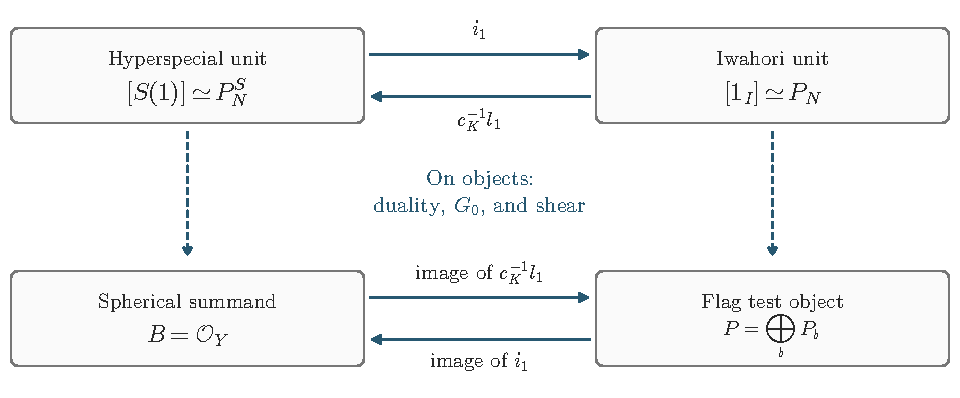
\includegraphics[width=.96\textwidth]{figures/local-comparison.pdf}
 \caption{The hyperspecial unit is a retract of the Iwahori unit.
 After coherent duality, the Koszul functor $G_0$, and shear, this
 becomes the retract $B=\cO_Y$ of the flag object $P$.
 The dashed arrows record the objects corresponding under these
 operations; duality reverses the solid arrows.  The comparison of
 representation-valued maps is \eqref{eq:hom-comparison}, and the
 resulting internal algebra comparison is \eqref{eq:spherical-end}.}
 \label{local:fig-retract}
\end{figure}

\begin{proof}
We first reconstruct the internal endomorphism algebra without
assuming that $L_S$ is a line.  The full corner embedding of
Lemma~\ref{trace:coend}, the retract
\eqref{trace:spherical-retract}, and the spherical loop calculation
of \cite[Proposition~2.7, ``Spectral form of a Frobenius trace'']{Parent}
give
\begin{equation}\label{eq:hom-comparison}
 \bigl(H^\bullet(B_{\rm sph}^0)\otimes V^*\otimes V'\bigr)^H
 \simeq
 \Hom^\bullet_{B^0,H}
       (L_S^0\otimes {V'}^*,L_S^0\otimes V^*)
\end{equation}
for neutral $L$-representations $V,V'$, restricted to $H$.  The order
on the right is reversed by $\mathbb D$; duality retains the displayed
Hom degree.  To justify base change in this formula, first make the
comparison on the two retracts in the trace.  Their invariant
coordinate rings agree by \eqref{eq:coordinate-shift}.  The etale
extension is flat and therefore tensors the cohomology of their
mapping complexes.  On the coherent side these complexes can be
computed after pullback to the slice, using degreewise finite free
resolutions against bounded targets and exact reductive
invariants.  The same comparison with compact source passes to
Ind-extensions by filtered colimits.  Finally $G_0$ is
$\cO(U_H)$-linear and respects representation tensors before shear;
duality takes constant tensors to their duals.  These facts give
\eqref{eq:hom-comparison} with the stated coefficients.

To recover the internal algebra, we need naturality of this
comparison for representation-valued maps, not just its displayed
vector-space isomorphisms.  Lemma~\ref{local:polynomial-representatives}
supplies the required representatives and proves their spectator
compatibility.  Its surjection is homogeneous for the original
polynomial degree, so it applies to every cohomological degree in
\eqref{eq:hom-comparison} before the shear as well.

In particular the comparison takes matrix maps with coefficients in
$\cO(U_H)$ to the same matrix maps, transposed by duality.  This
includes constant $H$-maps between restrictions of $L$-representations:
the strong slice expresses them as equivariant matrix functions on
the induced $L$-presentation.  Every representation of $H/Z(L)$
occurs as a summand of a restricted representation of $A$.  Indeed
matrix coefficients for the closed subgroup $H/Z(L)\subset A$ are
quotients of those for $A$, and complete reducibility extracts their
irreducible constituents.  The endomorphisms at issue have trivial
$Z(L)$-sector.  We may therefore use all these representation
summands in \eqref{eq:hom-comparison}.

Testing a rational $H$-module against all finite-dimensional
representations determines it.  Applying this observation to
\eqref{eq:hom-comparison} identifies
$H^\bullet(B_{\rm sph}^0)$ with the $H$-internal endomorphism
cohomology of $L_S^0$.  To recover multiplication, tensor the first
tested map with the representation coefficients of the second and
compose.  The spectator comparison proves that this is exactly the
tensor pairing defining internal composition.  Coefficients from
$\cO(U_H)$ give its scalar action by the same argument.  Duality may
reverse multiplication, which is harmless for the commutative
spherical ring.  Thus this is an algebra comparison over
$\cO(U_H)$, not merely a vector-space comparison of invariant Hom's.

After shear it gives \eqref{eq:spherical-end}, apart from the line
assertion.  Endomorphism degree changes by its $m$-weight.  Only even
weight sectors occur: the flag formula for $P$, and hence its retract
$L_S$, has this parity.  There is no completed internal Hom hidden
in this step.  After shear we have coherent modules on the affine
scheme $Y$ with reductive equivariance; bounded coherent targets
and resolutions finite in each degree compute the ordinary internal
endomorphism cohomology with its rational $H$-action.

We have proved that the internal endomorphism cohomology of $L_S$ is
commutative and concentrated in degree zero.  We next use the complete
intersection to deduce that $L_S$ is a line.  Let
\[
 i:Y\hookrightarrow U_H\times E_+
\]
be its regular equation embedding.  The ambient scheme is smooth,
so $i_*L_S$ is perfect there and $Li^*i_*L_S$ is perfect on $Y$.
The bimodule cohomology filtration of the derived tensor square of
$\cO_Y$ over the ambient ring has regular-sequence Tor terms.
Tensoring it with $L_S$ gives a finite filtration whose quotients are
$L_S$ tensored with exterior powers of the equation space, shifted
by $[j]$, for $0\le j\le\dim E_+$; its last quotient is the unshifted
$L_S$.  Locally these exterior factors are free.  Positive self-Ext
vanishing splits off the last quotient: the successive obstruction
groups have strictly positive degree.  Hence $L_S$ is locally a
summand of a perfect complex, and is perfect.

A minimal presentation over a local ring of a nonzero perfect complex
with two occupied degrees would give positive self-Ext: in the top
degree of the Hom complex, the last differential has entries in the
maximal ideal, so its cokernel remains nonzero modulo that ideal.
Thus $L_S$ is locally a vector bundle in a single degree.
Commutativity of its endomorphism algebra forces its rank to be at
most one.  The scheme $Y$ is connected, since $m$ contracts it to the
zero section over connected $U_H$.  The nonzero retract $L_S$
therefore has rank one throughout, with a locally constant shift.

We now remove the shift and trivialize the line equivariantly.
Take $u$ in a maximal torus of $H$, regular both for $H$ and for $tu$
in $L$, and remove the further resonances where
$\Ad(u)-1$ is singular on $E_+$.  On this dense torus locus the
flag formula for $P$ is an ordinary etale cover.  Its fibers have
trivial stabilizer-torus action and lie in degree zero.  The retract
$L_S$ consequently has zero shift and trivial torus character there.
Along the torus with $e=0$ this character is locally constant, so the
fiber at $(1,0)$ has trivial torus character.  Since $H$ is connected,
its one-dimensional character is then trivial.

Reductivity now gives an invariant section generating at $(1,0)$.
The affine quotient of $Y$ is the quotient of $U_H$, since the
$m$-weights contract all $e$-directions.  Every orbit over the identity
class has $(1,0)$ in its closure up to the unique closed orbit in that
fiber.  Thus an invariant section generating at $(1,0)$ generates
over this entire quotient fiber.  Its nongenerating locus is closed
and invariant, and its image in the affine quotient is closed.
Shrinking the saturated neighborhood removes that image.  The
section trivializes $L_S$, proving \eqref{eq:spherical-line} and the
last equality in \eqref{eq:spherical-end}.

It remains to verify the geometric compatibility of the ring
comparison.  It need not fix the $E_+$ coordinates literally,
but it is $H$-equivariant over $U_H$.  At $u=1$ its induced
automorphism preserves the unique open $H$-orbit in $E_+$ and hence
the boundary.  Suppose $u$ is unipotent and $e$ lies in that open
orbit.  The stabilizer $H_e$ is reductive, so $u$ can be contracted
to $1$ inside $H_e$.  If the image of $(u,e)$ under the coordinate
comparison had its vector in the boundary, equivariance and closedness
of the boundary would force the image of $(1,e)$ into the boundary
as well, a contradiction.  Applying the same argument to the inverse
gives the asserted preservation in both directions.
\end{proof}

\subsection{The local test available to global cohomology}

We collect the constructions in the form used in the remaining
sections.  In the statement, the equation embedding has conormal
bundle obtained from the finite $H$-representation $E_+^*$; this is
the source of the uniform finite filtrations used below.

\begin{theorem}\label{thm:local-test-model}
Let $t$, $H=Z_L(t)$ and $m$ be associated with a selected place as in
Lemmas~\ref{lem:test-places} and~\ref{lem:orbit-open}.
After an etale base change on invariant holonomy functions and a
saturated shrinking about the identity class, the Iwahori trace has a
fully faithful coherent realization.  Its composite with coherent
duality, the covariant Koszul functor $G_0$, and the change of degree
by $m$-weight is contravariant and has the following properties.

Its unit corresponds to
\[
 P=\bigoplus_bP_b\in\Coh^H(Y),\qquad
 Y=\{(u,e)\in U_H\times E_+:\Ad(u)e=e\},
\]
where the $P_b$ are the derived flag direct images in
\eqref{eq:flag-test}.  The scheme $Y$ is a classical complete
intersection in the smooth affine scheme $U_H\times E_+$.
The hyperspecial unit is the retract $B=\cO_Y$ of $P$ under
\eqref{eq:spherical-line}.  The unsheared representation comparisons
are \eqref{eq:hom-comparison}; their internal algebra and scalar
actions are \eqref{eq:spherical-end}.  Before duality the slide on a
label $V$ is the matrix $V(tu)$.

The ordinary $H$-equivariant algebra $\End(P)^{\rm op}$ is the affine
Hecke algebra with parameter $r$, pulled back along the etale map on
its center.  It has no higher cohomology, and its spherical corner is
$\End(B)=\cO(U_H)^H$.

All these comparisons respect the matrix operations, homogeneous
spherical maps, and neutral spectators of
Proposition~\ref{prop:trace-model}.  They permit tests by every
finite representation of $H/Z(L)$.  In the even sectors used below,
a test of $m$-weight $w$ changes cohomological degree from $b$ to
$b+w$; the other sectors use the stated parity adjustment.  The ring comparisons
preserve the open orbit and boundary over unipotent $u$.  The covariant
coherent and Koszul realizations extend fully faithfully to
Ind-completions; duality is applied to the compact test objects.

The same statements hold for finite products of selected places, with
external test objects, separate parity sectors, and the sum of the
$m$-weights.
\end{theorem}

\begin{proof}
The assertions at one place have been proved above and in
Proposition~\ref{prop:trace-model}.  On the chosen slice
$s=z^{-1}tu$, so the slide there is $V(zs)=V(tu)$.  Tensoring with a
representation commutes with the Koszul functor before shear;
duality replaces the representation by its dual.  An $m$-weight $w$
coefficient is shifted by $[-w]$ under shear, which gives the stated
degree change for its Hom test.  The ring and the flag objects have
even weights.  On an odd sector the additional subtraction of one
in the degree convention preserves even shifts, as in the definition
of shear.  The covariant Ind-extensions are fully faithful because they
are the colimit extensions of fully faithful functors on the coherent
compact objects.  Duality remains on these compact test objects.

For the endomorphism assertion, start with
Lemma~\ref{trace:hecke-algebra}, make the flat etale base change, and
apply the fully faithful Koszul comparison and duality.  Duality
reverses composition.  Equivariant maps have $m$-weight zero, so
shearing does not change their degree.  This proves the stated
identification with $\End(P)^{\rm op}$.  The spherical corner is
$\cO(Y)^H$ by \eqref{eq:spherical-line}; its equality with
$\cO(U_H)^H$ follows from the nonzero $m$-weights of the vector
coordinates.

For products, coherent Hom's of external objects satisfy K\"unneth:
use affine presentations, bounded coherent targets, resolutions with
finite terms in each degree, and exact reductive invariants.  The
constructible kernel products have the same equivariant K\"unneth
description, also obtainable from their orbit filtrations.  The cut
and coend calculations tensor together.  Thus the stable
idempotent-complete subcategory generated by external objects is
fully faithfully realized in coherent objects on the product.
This subcategory suffices for all subsequent tests; no assertion
that every coherent object is an external product is needed.
Shearing adds the weights from the different factors and keeps their
parity sectors separately.  This proves the product statement and
its Ind-extension.
\end{proof}


\section{A simultaneous lower bound}
\label{sec:lower-bound}

The local models of Section~\ref{sec:local-models} change a cohomological
degree by a weight of the cocharacters $m_i$.  We now prove that, after
localizing at the Hecke character of $f$, these changed degrees are
nonnegative.  The bound will hold for every finite collection of the
places chosen in Lemma~\ref{lem:test-places}, with the same lower bound
zero.  This uniformity permits the simultaneous tests in
Section~\ref{sec:boundary}.

Fix distinct places $x_1,\ldots,x_n$ from that sequence, with $n\geq1$, and
put
\[
 T_I=\{x_1,\ldots,x_n\},\qquad U'=U\setminus T_I,
 \qquad \Gamma'=W_{U'},\qquad d_i=\deg(x_i).
\]
At the places of $T_I$ we use Iwahori level; elsewhere we retain the full
level $D$.  Let $\mathsf K_I$ be the fixed-place path functor at this level.
As before, $y_0\in U\setminus T_I$ is the auxiliary place, and $C$ is its
full spherical Hecke algebra.  Write $\mathfrak m_C$ for the maximal ideal
of $C$ determined by $f$.  All absolute values in this section are taken
in one fixed complex realization.

For neutral representations $V_i\in\Rep(L)$, set
\begin{equation}
 N_b(V)=H^b\mathsf K_I\!\left(\boxtimes_{i=1}^n Z(V_i)\right),
 \qquad V=\boxtimes_{i=1}^nV_i.
 \label{bounds:unsheared}
\end{equation}
There is one nontrivial label at the selected geometric point of each
Frobenius cycle and a unit label at its other points.  If $D_*$ is divisible
by all the $d_i$, \emph{complete Frobenius through degree $D_*$} means the
product of the full-cycle slides, with their Weil structures, raised in
the $i$th factor to the power $D_*/d_i$.

The numerical comparison behind the bound is already visible in the
local model.  Retain its centralizer $H_i$ and cocharacter $m_i$ at
$x_i$, and let $W_i\subset V_i^*$ be an irreducible $H_i$-summand in
the even $m_i(-1)$-sector.  If $w_i$ is its $m_i$-weight and
$w=\sum_iw_i$, duality and the change of grading replace degree $b$
by $b+w$.  At the slice-center value $[u_i]=[1]$ for every $i$, the
complete-Frobenius eigenvalues on this dual-label test have modulus
$q^{-D_*w/2}$.  We will prove the arithmetic inequality
\[
                         |\alpha|\leq q^{D_*b/2}
\]
after quotienting $N_b(V)$ by $\mathfrak m_C$ and localizing at the
away Hecke values of $f$.  A nonzero test satisfying both bounds must
have $b+w\geq0$.  The next two subsections establish the arithmetic
inequality by simultaneous degeneration and constituent purity; we
then apply it to the coherent tests and pass to ordinary
quasi-coherent complexes.

\subsection{Disjoint Hecke actions and simultaneous degeneration}

The path functor and moving-leg cohomology carry Hecke operations in two
apparently different descriptions.  Their agreement is needed before
we use finite generation.

\begin{lemma}\label{bounds:disjoint-hecke}
At a place carrying a unit path label, the spherical trace action on
$\mathsf K_I$ agrees with the usual disjoint Hecke action on compact
shtuka cohomology, with the Satake conventions fixed in
Section~\ref{sec:global-support}.  This agreement holds with arbitrary
labels and full or parahoric levels at the other places.
\end{lemma}

\begin{proof}
Both actions use the same modification correspondence and the
Weil-stalk trace at the auxiliary place.  One can check the normalization
after temporarily imposing Iwahori level there.  For a closed simple-wall
kernel, the parallel-wall calculation of \cite[Proposition~2.6]{Parent},
applied at position the identity, gives pullback
followed by summation over Frobenius-fixed rank-one flag refinements.
This is the ordinary Hecke correspondence; subtracting the identity
gives the simple generator.  A length-zero kernel gives the graph of a
unique transport, with coefficient one for its unshifted constant
sheaf.  These kernels generate the Iwahori Hecke algebra.

Transfer between Iwahori and hyperspecial level is similarly pullback
and summation over Frobenius-fixed full flags, with the index
normalization in \cite[Proposition~2.6]{Parent}.  All other modification labels
are carried unchanged through these diagrams.  Since there is no leg at
the auxiliary place, the Frobenius-fixed flags are finite \emph{\'etale}
in families; a further finite level there trivializes them.  Thus the
calculation is compatible with the other levels and with compact direct
image.
\end{proof}

To compare all the central labels in \eqref{bounds:unsheared} at once, we
place their degenerations over a single rational point of a second
curve.  The following elementary choice of map is useful.

\begin{lemma}\label{bounds:curve-map}
For disjoint finite sets $T_I,\supp(D),\{y_0\}\subset|X|$, there is a
finite generically separable morphism
\[
 \pi:X\longrightarrow\mathbb P^1_{\F_q}
\]
unramified over $0,1,\infty$, such that $T_I$ lies above $0$, $\supp(D)$
lies above $\infty$, and $y_0$ lies above $1$.
\end{lemma}

\begin{proof}
Take high powers of an ample line bundle and choose sections $s,t$ with
prescribed first jets at the indicated points.  Prescribe simple zeros
of $s$ at $T_I$, simple zeros of $t$ at $\supp(D)$, and simple zeros of
$s-t$ at $y_0$, keeping the other necessary values nonzero.  These
conditions can be imposed over the residue fields, and force $s$, $t$,
and $s-t$ to be nonzero sections.  We seek a pair with no common zero
and with each of these three sections having only simple zeros.  Then
$[s:t]$ is the required morphism.

Here is the finite-field existence argument.  At any fixed finite set
of additional closed points, Riemann--Roch makes the jet conditions
independent once the degree of the line bundle is large.  The local
probability of satisfying the conditions is positive, including over
residue fields with two elements: one can choose the two first jets
with nonzero determinant.  At a point of degree $l$ outside the
prescribed set, a forbidden double zero or common zero has probability
$O(q^{-2l})$, with a constant independent of the line-bundle degree.
Indeed, for a line bundle of degree $m$ the dimension bound
\[
 h^0(\mathcal L(-2x))\leq\max(0,m-2l+1)
\]
gives this estimate for double zeros, and the analogous bound for
$\mathcal L(-x)$ gives it for common zeros.  The fixed jet prescriptions
affect only the constant.  If the required order of vanishing is
impossible for a nonzero section, its probability is zero.  Since the
number of degree-$l$ points is $O(q^l)$, the sum of the excluded tail
probabilities tends to zero.  The product of the positive local
probabilities therefore has positive limit.  A suitable pair exists.
Its simple zero at any point of $T_I$ also ensures generic separability.
\end{proof}

\begin{proposition}\label{bounds:nearby}
For any finite $T_I$ and neutral labels $V_i$, the groups $N_b(V)$ are
finitely generated $C$-modules.  There is a finite set of additional
places which can be omitted from the away Hecke actions such that the
following comparison holds.  For a sufficiently divisible $D_*$,
$N_b(V)$ identifies, compatibly with $C$, the remaining away Hecke
actions, and complete Frobenius, with a direct summand of moving-leg
cohomology at the same level over a geometric generic tuple in
$(U')^n$.  On the latter group complete Frobenius acts through a tuple
in $(\Gamma')^n$ whose degree is $D_*$ in every factor.
\end{proposition}

\begin{proof}
We use the one-leg case of the characteristic-zero parahoric
comparison of \cite[Theorem~5.2(1)]{Bounds:SalmonNearby}.  Its setting
allows a smooth affine group scheme over a curve with quasi-split
reductive generic fiber, parahoric reduction at the degenerating point,
and arbitrary full level away from that point, encoded by dilatation.
For one moving Satake leg, with a stationary unit label omitted, the
canonical comparison is an isomorphism
\begin{equation}
 p_!\Psi\mathcal S\ \xrightarrow{\ \sim\ }\ \Psi p_!\mathcal S.
 \label{bounds:nearby-comparison}
\end{equation}
Here $\Psi$ is the full trait nearby-cycle functor and $p_!$ is the
filtered limit over Harder--Narasimhan bounds.  The assertion is made
on this limit itself: the fusion and partial-Frobenius constructions
of \cite[Proposition~3.5, Theorem~3.8, and Lemma~4.2]{Bounds:SalmonNearby}
apply to the resulting ind-constructible complexes.  Creation of a
dual pair of Satake legs, fusion of nearby cycles, and annihilation
construct an inverse, whose two compositions with the canonical map
are the tensor evaluation--coevaluation identities
\cite[Lemma~4.6, Corollary~4.7, and proof of Theorem~5.2]{Bounds:SalmonNearby}.
Thus this characteristic-zero comparison is established directly on
the Harder--Narasimhan limit.

We use the canonical map in \eqref{bounds:nearby-comparison} for all
equivariance statements.  It respects the full local Galois action
and the Weil descent data; its inverse consequently does too.  This
does not require separate local Weil equivariance of every auxiliary
fusion map used to construct the inverse
\cite[paragraph following Lemma~4.6 and Corollary~6.1]{Bounds:SalmonNearby}.
All coefficients and labels can be taken over a sufficiently large
finite extension $E$ of $\Q_\ell$.

Choose $\pi$ as in Lemma~\ref{bounds:curve-map}.  Enlarge $D$ to
$\pi^*(m_\infty\infty)$ for $m_\infty$ large enough.  We will recover the
original level by finite level-group invariants.  Let $\mathcal G$ be
the smooth group scheme on $X$ with Iwahori fibers at $T_I$ and
hyperspecial fibers elsewhere, and take its Weil restriction to
$\mathbb P^1$.  This is smooth affine with connected geometric fibers
and quasi-split semisimple generic fiber: restriction of a split Borel
becomes a product of Borels over a separable closure.  It is parahoric
also at the branch places: under finite separable extension of complete discretely valued
fields, the building and facet identification, with rescaled
valuation, identifies the Weil restriction of a parahoric model with
the corresponding parahoric model.  This is the Weil-restriction
property of Bruhat--Tits models; see
\cite[Appendix~F, Fact~F.1]{Bounds:KalethaWeilRestriction}, which
allows extensions that are not tamely ramified.  Connectedness can also be checked on
the local fibers, where the additional congruence groups are
geometrically unipotent.  The full level $m_\infty\infty$ can be encoded by dilating this
model at the identity along that divisor, as in
\cite[Section~2]{Bounds:SalmonNearby}.  This leaves the model at $0$
unchanged.  Thus the hypotheses of \eqref{bounds:nearby-comparison}
hold, with degeneration at $0$ and the enlarged full level at
$\infty$.

Over the strict local curve at $0$, the cover $X\to\mathbb P^1$ splits
into its geometric branches.  On the branches selected by the $x_i$
we place the labels $V_i$; on the other branches we place the unit.
To apply the global theorem, first induce this external tensor label
from the connected dual group to its semidirect product with the finite
splitting group.  This amounts to taking its finite family of
translates, with permutation descent.  After restriction to the strict
local curve, the original external tensor is a summand.  Naturality of
the canonical map \eqref{bounds:nearby-comparison} permits projection
onto this summand, although that summand need not descend separately
over the global good open.  Increasing $D_*$ makes Frobenius preserve
every selected summand.  The relative Satake normalization splits as
the product of the normalizations on the branches; any common base
shift or twist in a convention is compensated on both sides.  Neutral
labels have no component-parity correction.

For completeness, the integral comparison cone in this particular
application also vanishes.  Choose an $\mathcal O_E$-Satake lattice in
the induced label, and keep the full level at $\infty$ separate from
the parahoric model.  Let $\mathcal C_{\mathcal O_E}$ be the cone of
\eqref{bounds:nearby-comparison} for that lattice, before taking
finite level-group invariants or rational summands.  Reduction modulo
the uniformizer $\varpi$ and extension of coefficients to $E$ commute
with this comparison: on its source, compute constructible trait
nearby cycles and compact direct image on finite-type charts and
then pass to the filtered Harder--Narasimhan limit; on its target,
nearby cycles on the curve base itself are the geometric generic
fiber.  Apply the torsion case of
\cite[Theorem~2.2]{Bounds:EteveXueNearby} with a stationary unit leg
and constant coefficient on its restricted-shtuka factor at $0$.
Writing $k_E=\mathcal O_E/(\varpi)$, it gives
\[
 \mathcal C_{\mathcal O_E}\otimes^L_{\mathcal O_E}k_E=0.
\]
Multiplication by $\varpi$ on this cone is consequently invertible,
so
\[
 \mathcal C_{\mathcal O_E}
   \simeq\mathcal C_{\mathcal O_E}\otimes_{\mathcal O_E}E
   \simeq\mathcal C_E=0,
\]
where the last equality is the independent characteristic-zero
comparison just proved.  This argument applies to the actual
one-leg Satake coefficient used here.  It makes no completion
assertion about general Hecke-finite modules.  In the remainder of
the proof all invariants and selected summands are taken over $E$,
where they preserve the comparison isomorphism.

The resulting generic shtuka cohomology is the moving-leg cohomology
on $X$ along the branch tuple.  Indeed torsors for the Weil restriction
are equivalent to torsors on the finite cover.  This can be checked
\'etale locally on the base: over a strict henselian local base a
smooth torsor on the finite cover trivializes \emph{\'etale} locally.
The equivalence works with arbitrary base schemes and commutes with
the Frobenius pullback in the shtuka diagram.  Modification data agree
away from the branch locus and, near $0$, by the split description.
Level structures agree by definition.  Consequently these
identifications commute with an exhaustion by finite-type opens.

On the special fiber, the local-model morphism for shtukas is smooth
after sufficient truncation on each bounded modification.  Nearby
cycles therefore pull back from the Beilinson--Drinfeld Grassmannian
for the parahoric group scheme.  A spherical modification degenerating
to an Iwahori place gives the central sheaf $Z(V_i)$, with unit flag
label, by its nearby-cycle construction
\cite[Theorem~2.3]{Parent}.  If $Z$ is
defined using unipotent nearby cycles, retain that summand.  The
K\"unneth isomorphism for nearby cycles over a trait, on bounded
supports, tensors these calculations across the split branches.
Although the trait has diagonal inertia on the product, the
factorwise unipotent projections are still defined.  They are stable
under a sufficiently divisible Frobenius power.  This gives precisely
the central coefficients in \eqref{bounds:unsheared}, with its path
normalization, as a summand of the comparison.

The special-fiber Frobenius in this construction is the product of
the slides in \eqref{bounds:unsheared}, by cyclicity of the path functor
\cite[Proposition~2.5, Coherent path rotation]{Parent}.  A change of
local Frobenius lift does not change its spectrum.  On the unipotent
nearby-cycle summand, inertia acts through tame logarithmic monodromy
$N$, and Frobenius conjugates $N$ by a nontrivial power of $q$ or its
inverse.  Multiplying a Frobenius lift by $\exp(cN)$ thus conjugates it
by another exponential of $N$.  The same argument works separately
on the factors and commutes with disjoint Hecke operations.  The
branches give the same strict local curves as the coordinates used
earlier to construct the path functor.

We may omit from the away Hecke actions all places over $0$ and
$\infty$.  Every remaining Hecke correspondence is disjoint from the
degeneration; it is finite \emph{\'etale} after the usual level
refinement and carries the modification coefficient along unchanged.
Hence \eqref{bounds:nearby-comparison} is equivariant for it, in
particular for $C$ at $y_0$.  Taking finite level-group invariants at
$\infty$ now recovers the original level $D$.  These invariants are
exact and commute with the comparison.

To make the passage from the branch tuple to independent moving legs
explicit, let $\xi$ be a geometric generic point of the trait at $0$,
and let $\alpha:\xi\to(U')^n$ be its selected branch tuple.  This
tuple need not be generic in the product.  Choose a geometric generic
specialization $\overline\eta_n\to\alpha$ in $(U')^n$.
The specialization isomorphism of
\cite[Theorem~4.2.3]{Bounds:XueSmoothness} identifies the fiber of
each ind-smooth cohomology sheaf at $\alpha$ with its fiber at
$\overline\eta_n$.  On the latter fiber,
\cite[Theorem~2]{Bounds:XueFiniteness} applies: its restriction
excluding nonzero Frobenius graphs is satisfied at this generic
point.  This proves finite generation over $C$.

These identifications also retain the actions.  For any finite
collection of away Hecke operations, restrict the leg positions to
the open avoiding their places.  Both $\alpha$ and
$\overline\eta_n$ lie in this open, and specialization is natural
for the Hecke morphisms there.  Taking the filtered union handles all
the away operations, and hence their quotients and localizations.
By the product Weil action in
\cite[Proposition~5.0.4]{Bounds:XueSmoothness}, recalled in
Lemma~\ref{lem:glob-cohomology}, the local Weil action pulled back
along $\alpha$ is the product of its coordinate branch actions.
Because $\pi$ is unramified over $0$, after $D_*$ fixes the branches
the $i$th action is a local lift of
$\Frob_{x_i}^{D_*/d_i}$.  Its degree is therefore $D_*$.
Changing the paths used in specialization conjugates these lifts
and leaves their degrees unchanged.  This proves every assertion.
\end{proof}

\subsection{The constituents after imposing Hecke values}

Proposition~\ref{bounds:nearby} does not by itself transfer a weight
bound from ordinary fibers to nearby cycles.  We obtain that bound by
first identifying the possible irreducible Weil constituents after
imposing the Hecke values of $f$.

Fix $b$ and work at the Iwahori level above.  In the regular module
$M_b^{\mathrm{reg}}$ of Section~\ref{sec:global-support}, first quotient
by $\mathfrak m_C$ and then localize at the joint neutral spherical
Hecke values of $f$ outside the finite exceptional set of
Proposition~\ref{bounds:nearby}.  Denote the result by $M'$.  Each of its
$A$-isotypic pieces is finite dimensional.  On each such piece the
localization simply retains the corresponding joint primary summand.
The neutral algebra at a place is $k[A]^A$, acting by the Hecke
identity.  Define the finite-dimensional $(\Gamma')^n$-module
\[
 D_b=\left(M'\otimes\bigotimes_{i=1}^n V_i\right)^A.
\]
By \eqref{eq:regular-tests} and exactness of $A$-invariants, $D_b$
is the generic moving-leg cohomology with labels $V_i$ after the same
$C$-quotient and away Hecke localization.  Proposition~\ref{bounds:nearby}
therefore identifies the corresponding reduction of $N_b(V)$ with
a direct summand of $D_b$, equivariantly for the complete Frobenius
given there by a tuple of local Weil lifts.  It suffices to control
the constituents of $D_b$ to bound the spectrum on that summand.

\begin{proposition}\label{bounds:constituent-inclusion}
Every irreducible constituent of $D_b$ occurs among the constituents of
\begin{equation}
 \boxtimes_{i=1}^n\bigl(V_i\circ\sigma_{\nu,\mathrm{ad}}\bigr)
 \bigm|_{(\Gamma')^n}.
 \label{eq:constituents}
\end{equation}
This assertion concerns occurrence of constituents and does not
prescribe their multiplicities.
\end{proposition}

\begin{proof}
Let $\mathscr B_{\Gamma'}$ be the coordinate algebra of
$\Hom(\Gamma',A)$ used in Section~\ref{sec:global-support}, with
$\Gamma'$ regarded as an abstract group.  It acts on $M'$.  Choose
finitely many coefficient vectors of a basis of $D_b$, take their
$A$-spans, and let $M''\subset M'$ be the
$\mathscr B_{\Gamma'}$-module they generate.  Put
\[
 R'=\mathscr B_{\Gamma'}/\operatorname{Ann}(M'').
\]
This algebra is of finite type.  To see this, choose finitely many
representations whose matrix entries generate $k[A]$.  Their matrix
entries, as the Weil element varies, carry the chosen generating
vectors into a fixed finite list of $A$-isotypics.  Those isotypics are
finite dimensional after the $C$-quotient.  Thus the span of these
entries in $R'$ is finite dimensional: vanishing of an operator is
tested on the generating vectors and their $A$-spans, since all
coordinate operators commute.  Finitely many entries therefore
generate $R'$.

At any $k$-point of $R'$, the universal matrices specialize to a
homomorphism $b':\Gamma'\to A(k)$.  This homomorphism is continuous and
defined over a finite extension of $\Q_\ell$.  Indeed the entries are
finite-dimensional linear evaluations of their actions on the
generating spaces.  Testing those actions by
\eqref{eq:regular-tests} uses only a fixed finite list of representation
labels.  The resulting finite-dimensional quotients carry the
continuous partial Weil actions of Lemma~\ref{lem:glob-cohomology}.
The chosen primary summands are determined, on these finitely many
spaces, by finitely many Hecke equations.  Enlarging the coefficient
field accommodates these equations and the finitely many coordinates
of the $k$-point.

For every away place used in the localization, the Hecke identity
shows that
\[
 [b'(\Frob_y)]^{\mathrm{ss}}
   =[\sigma_{\nu,\mathrm{ad}}(\Frob_y)]^{\mathrm{ss}}.
\]
Indeed a power of each prescribed class-function difference kills the
generators of $M''$, hence all of $M''$, and vanishes at every point
of $R'$.  These Frobenius eigenvalues are $\ell$-adic units.  The
geometric image of $b'$ is compact by continuity.  In a faithful
matrix representation, the powers of one such Frobenius also have
compact closure.  If $h\in\Gamma'$ has degree one and this Frobenius
has degree $d$, then $b'(h)^d$ differs from its image by an element of
the compact normal geometric image.  Its powers, and therefore all
powers of $b'(h)$, have compact closure.  The degree splitting now
extends $b'$ continuously to $\pi_1(U')$.

Chebotarev and the ordinary character criterion imply that, in every
algebraic representation, $b'$ and $\sigma_{\nu,\mathrm{ad}}$ have the
same semisimplification on $\pi_1(U')$.  The latter representation is
semisimple because the parameter has reductive Zariski closure; the
same remains true on the dense Weil group.  Thus the assertion of the
proposition holds after specialization at every $k$-point of $R'$.

It remains to pass from these pointwise statements to $D_b$.  Let
$J$ be the annihilator in the ordinary group algebra
$k[(\Gamma')^n]$ of the semisimple representation
\eqref{eq:constituents}.  The universal matrices over $R'$ give an
action on $\bigotimes_i V_i$.  At every $k$-point, $J$ kills each
successive composition factor, so $J^r$ acts by zero there for an
integer $r$ bounded by the dimension of that tensor product.  Its
matrix entries therefore lie in the nilradical of $R'$.  Since $R'$
is noetherian, a further power of $J$ acts by zero over $R'$ itself,
and hence on $D_b$.  The quotient $k[(\Gamma')^n]/J$ is the
finite-dimensional semisimple image algebra of
\eqref{eq:constituents}.  Its simple modules are precisely the
constituents appearing there, which proves the claim.
\end{proof}

\begin{proposition}\label{bounds:weight-bound}
Quotient $N_b(V)$ by $\mathfrak m_C$ and localize at the neutral
spherical Hecke values of $f$ outside the finite exceptional set in
Proposition~\ref{bounds:nearby}.  On the resulting finite-dimensional
space, every eigenvalue $\alpha$ of complete Frobenius through a
sufficiently divisible degree $D_*$ satisfies
\begin{equation}
 |\alpha|\leq q^{D_*b/2}.
 \label{bounds:frobenius-weight}
\end{equation}
\end{proposition}

\begin{proof}
Every irreducible constituent of each factor of
\eqref{eq:constituents} is lisse on all of $U$, is defined over a
finite extension of $\Q_\ell$, and has algebraic Frobenius
eigenvalues.  The constituent argument in
\cite[Lemma~6.4]{Parent}
therefore gives a single pure weight for that constituent at every
point of $U$.  More explicitly, its determinant is made finite order
by an algebraic constant-field twist; purity of the twisted
irreducible sheaf then shows that every eigenvalue of the original
constituent has the same exponent, independent of the place.  This
argument permits arbitrary ramification outside $U$.

Choose pairwise disjoint closed points for the moving legs in $U'$,
and take complete Frobenius through a common multiple of their
degrees.  By \eqref{eq:regular-tests}, smooth transport, and
Lemma~\ref{lem:glob-weights}, $D_b$ is a subquotient to which the
compact-cohomology weight bound applies.  Thus the sum of the pure
weights in every occurring external-tensor constituent is at most
$b$.  The Hecke quotient and localization can be performed at a
geometric generic point; this argument only transports their
resulting Weil subquotient and does not require Hecke modifications
at a colliding leg.

The same constituents extend across all the points of $T_I$, by
Proposition~\ref{bounds:constituent-inclusion}.  Consequently the
tuple of local Frobenius lifts in Proposition~\ref{bounds:nearby}
has, on each constituent, the same sum weight as the disjoint good
tuple.  This gives \eqref{bounds:frobenius-weight} for the nearby-cycle
comparison and its direct summand $N_b(V)$.
\end{proof}

\subsection{Central localization and the change of grading}

We now apply this spectral inequality to the coherent models.  Exact
representability on the compact trace categories, with the duality of
Section~\ref{sec:trace}, gives an Ind-object $F_N$ characterized by
\begin{equation}
 \mathsf K_I(J)=\RHom\bigl(\mathbb D[J],F_N\bigr).
 \label{eq:global-functional}
\end{equation}
This is the same representability argument as in
\cite[proof of Proposition~2.7]{Parent}, applied to the finite tensor product of the
compact categories in Proposition~\ref{prop:trace-model}.  All Hom
complexes are taken equivariantly.  Pull $F_N$ to the chosen \emph{\'etale}
slices at $x_i$.  We retain the sectors with trivial action of
$Z(L)^n$, so the acting group becomes
\[
 H^\natural=\prod_{i=1}^n H_i/Z(L).
\]
We also retain the sectors with trivial action of every $m_i(-1)$.
The flag and spherical objects in Theorem~\ref{thm:local-test-model}
belong to these sectors.

Let $\mathcal Z$ be the tensor product of $C$, the neutral spherical
algebras at all other places of $U\setminus T_I$, and the slice-center
rings $k[U_{H_i}]^{H_i}$.  An infinite tensor product here means the
filtered union of its finite tensor products.  Its character is given
by the Hecke values of $f$ and by the identity classes $u_i=1$ on the
slices; denote the corresponding maximal ideal by $\mathfrak m$.

\begin{lemma}\label{bounds:central-actions}
The algebra $\mathcal Z$ acts on the representing Ind-object by
commuting dg endomorphisms.  Pullback to the slices and localization at
$\mathfrak m$ commute with mapping from compact objects.  In
particular, the latter operation computes ordinary flat localization
on the cohomology of the mapping complexes.
\end{lemma}

\begin{proof}
The slice-center rings act centrally on the coherent models.  For the
away factors, include any finite disjoint list of additional places
in the path functor with spherical labels, then restrict to the unit
label at those places in the horizontal trace.  The endomorphisms of
these units carry the ordinary spherical algebra action computed by
the loop model in \cite[Proposition~2.7]{Parent}.  They therefore act on
the functor on the remaining trace compacts and hence on $F_N$.

These actions commute and are compatible as the finite list grows.
Indeed insertion of further unit labels compares the external
products of the balanced bar constructions defining the traces;
their unit-insertion identities give the required coherence.  Thus
they define an action of the filtered union $\mathcal Z$ itself.
Lemma~\ref{bounds:disjoint-hecke} identifies these actions on mapping
cohomology with the disjoint Hecke actions already used above.
The \emph{\'etale} comparisons respect these scalars by
Section~\ref{sec:local-models}.  Finally localization is tensoring
with the flat algebra $\mathcal Z_{\mathfrak m}$, and a compact
source commutes with the colimits computing this tensor product.
\end{proof}

Apply this localization and the Koszul functors and cohomological
change of grading of Theorem~\ref{thm:local-test-model}, extended to
Ind-categories.  The order of localization and these functors is
immaterial.  Denote the resulting object by
\[
 F^{\mathrm{ind}}\in
 \Ind\!\left(\Coh^{H^\natural}\!\left(\prod_{i=1}^nY_i\right)\right).
\]
Set $P=\boxtimes_iP_i$ and $B=\mathcal O_{\prod_iY_i}$.
By \eqref{eq:spherical-line}, $B$ is the selected spherical summand
of $P$.  The change of grading uses the sum of the $m_i$-weights.

\begin{theorem}[Simultaneous lower bound]
\label{thm:simultaneous-bound}
For every finite collection of the chosen places and every finite
algebraic representation $W$ of $H^\natural$, one has
\begin{equation}
 \RHom(P\otimes W,F^{\mathrm{ind}})\in D^{\geq0}(k).
 \label{eq:lower-bound}
\end{equation}
The lower bound zero is independent of the collection of places and
of $W$.
\end{theorem}

\begin{proof}
It suffices to consider irreducible $W$.  Representations in the
discarded parity sectors give zero.  Every remaining $W$ occurs in
the restriction of $V^*$ for some external tensor of neutral
$L$-representations $V_i$, by the restriction statement of
Theorem~\ref{thm:local-test-model}.  Before the change of grading,
\eqref{eq:global-functional} and the local comparison identify its
mapping groups with the $W$-summand of
\eqref{bounds:unsheared}, pulled to the slices and localized.  Here
$[Z(V_i)]$ corresponds to $P_{N,i}\otimes V_i$ and
$\mathbb D P_{N,i}=P_{N,i}$.  If $m_i$ has weight $w_i$ on $W$, put
$w=\sum_iw_i$.  A class in the original cohomological degree $b$
has degree $b+w$ after the change of grading: the changed source
with label $W$ is $(P\otimes W)[-w]$.

The original degree-$b$ mapping group is finitely generated over
$\mathcal Z_{\mathfrak m}$.  Before the slice extension this follows
from Proposition~\ref{bounds:nearby}, since a finite set of
$C$-generators also generates over the larger central algebra.
The \emph{\'etale} extension preserves finite generation because we
retain its slice-center scalars; taking a representation summand
preserves it as well.  We may therefore prove vanishing by reduction
modulo $\mathfrak m$ and Nakayama's lemma.  No noetherian hypothesis
on the infinite tensor product $\mathcal Z$ is needed here.

The bound \eqref{bounds:frobenius-weight} persists on this reduction.
First quotient by $\mathfrak m_C$ and localize at the away places
used in Proposition~\ref{bounds:weight-bound}; then perform the
remaining central reductions and base changes.  These operations
commute with complete Frobenius.  On the slice, the Frobenius action
is the matrix action on the coherent representation labels, as in
Section~\ref{sec:local-models}.

More precisely, before duality its action on the $i$th label is
\begin{equation}
 V_i\bigl((t_iu_i)^{D_*/d_i}\bigr).
 \label{bounds:matrix-frobenius}
\end{equation}
Dualizing an endomorphism means that on $V_i^*$ one uses the
representation matrix with inverse group argument, acting on the
Hom complex by precomposition.  This operator preserves each
$H_i$-summand, since $t_iu_i\in H_i$.  Its characteristic polynomial
has coefficients in the slice-center ring, and the same polynomial
identity holds on the mapping groups.  At the central value
$[u_i]=[1]$, every eigenvalue on the $W$-summand consequently has
absolute value
\[
 q^{-wD_*/2},
\]
because the absolute-value direction of $t_i$ is $m_i/2$, with
base $q^{d_i}$, by Lemma~\ref{lem:test-places} and
Section~\ref{sec:open-orbit}.  Unipotent $u_i$ does not change these
eigenvalues.

If $b+w<0$, this absolute value is strictly larger than
$q^{bD_*/2}$, contrary to \eqref{bounds:frobenius-weight}, unless
the reduced mapping group is zero.  Nakayama's lemma then makes
the original localized group zero.  This proves
\eqref{eq:lower-bound}.  Although the sufficiently divisible integer
$D_*$ may depend on the finite collection and the labels, the
inequality $b+w\geq0$ does not, giving the asserted uniformity.
\end{proof}

\subsection{Passage to ordinary quasi-coherent complexes}

Let $F^{\mathrm{qc}}$ be the image of $F^{\mathrm{ind}}$ under the
natural functor from Ind-coherent objects to ordinary equivariant
quasi-coherent complexes on $\prod_iY_i$.  The next proposition
specifies exactly which mapping complexes survive this passage.

\begin{proposition}\label{prop:ind-qc-comparison}
The complex $F^{\mathrm{qc}}$ is concentrated in degrees at least
zero.  If $Q$ belongs to the thick subcategory generated by the
objects $P\otimes W$, for finite representations $W$ of
$H^\natural$, then the natural comparison is an isomorphism:
\begin{equation}
 \RHom(Q,F^{\mathrm{ind}})
   \xrightarrow{\ \sim\ }\RHom(Q,F^{\mathrm{qc}}).
 \label{eq:ind-qc-comparison}
\end{equation}
\end{proposition}

\begin{proof}
For a perfect source, the comparison is automatic.  Apply
Theorem~\ref{thm:simultaneous-bound} to the summand $B$ of $P$ and
all its representation twists.  Since reductive invariants are
exact, these tests detect the ordinary cohomology of
$F^{\mathrm{qc}}$.  They show that it lies in degrees at least
zero.

Fix $Q$ as in the statement.  The left side of
\eqref{eq:ind-qc-comparison}, even after replacing $Q$ by
$Q\otimes W$ for arbitrary finite $W$, has a uniform lower bound:
start with Theorem~\ref{thm:simultaneous-bound} and use the finitely
many cones, shifts, and retracts constructing $Q$.  The right side
also has a uniform lower bound, since $Q$ is bounded coherent and
$F^{\mathrm{qc}}\in D^{\geq0}$.

Let $i$ be the regular equation embedding of $\prod_iY_i$ into the
smooth ambient space from Section~\ref{sec:local-models}.  Its
conormal bundle is the structure sheaf tensored with a finite
representation.  The complex $Li^*i_*Q$ is perfect, because $i_*Q$
is bounded coherent on that smooth ambient space.  The finite
Postnikov filtration of the self-intersection bimodule gives a
filtration of $Li^*i_*Q$ whose final quotient is $Q$ and whose other
quotients are
\[
 Q\otimes W_j[j],\qquad j>0,
\]
for the exterior powers $W_j$ of the conormal representation.  This
uses the regular-sequence formula for the Tor groups; it requires
no splitting of the self-intersection bimodule.

For a source $T$, let $E(T)$ be the cone of the comparison
\eqref{eq:ind-qc-comparison}.  Suppose some $E(Q\otimes W)$ is
nonzero.  The uniform lower bounds give a least integer $h$ in
which one of these cones has nonzero cohomology.  Choose such a
$W$ and apply the preceding filtration to $Q\otimes W$.
Contravariance gives
\[
 E(T[j])=E(T)[-j],
\]
so all its positive-$j$ pieces have cohomology only in degrees
at least $h+j$.  The final unshifted quotient therefore supplies
an injection
\[
 H^h E(Q\otimes W)
 \lhook\joinrel\longrightarrow H^hE(Li^*i_*(Q\otimes W)).
\]
The target is zero because its source is perfect.  This
contradiction proves the comparison.
\end{proof}

In particular, the canonical map
$H^0(F^{\mathrm{qc}})\to F^{\mathrm{qc}}$ is available, and maps
from finite constructions using the flag and spherical summands of
$P$ can be tested in ordinary quasi-coherent complexes.  Both facts
will be used in Section~\ref{sec:boundary}.


\section{Simultaneous boundary tests and completion of the proof}
\label{sec:boundary}

We now compare the two consequences of a failure of enhancement.  By
Proposition~\ref{prop:open-orbit-enhancement}, such a failure confines the
finite type support $\Spec R$ to the boundary of the open orbit at every
selected place.  We shall construct a coherent test at each place whose
map to the spherical summand vanishes on every derived fiber over this
support.  Noetherianity then makes a finite product of these maps vanish
on the whole support.  The cuspidal vector $f$, however, survives every
such product, as we shall see from a simple quotient of its Iwahori
Hecke module.

Throughout this section, assume that the occurring excursion character
$\nu$ has no enhancement as in Theorem~\ref{thm:main}.  Retain the
nonzero eigenvector $f$ and its cyclic support algebra $R$ from
Proposition~\ref{prop:global-support}, together with the infinite sequence
of places $x_i$ from Lemma~\ref{lem:test-places}.  At $x_i$ write
\[
 r_i=q^{\deg x_i},\qquad H_i=Z_L(t_i),\qquad
 E_i=\ker(\Ad(t_i)-r_i),\qquad H_i^\natural=H_i/Z(L).
\]
Let $m_i$ be the cocharacter of the prescribed triple.  The local models
of Theorem~\ref{thm:local-test-model} are
\[
 Y_i=\{(u,e)\in U_{H_i}\times E_i:\Ad(u)e=e\},\qquad
 B_i=\cO(Y_i),\qquad P_i=\bigoplus_b P_{i,b}.
\]
Here $b$ runs through the components of the $t_i$-fixed flag variety, and
$P_{i,b}$ is the derived incidence pushforward in
\eqref{eq:flag-test}.  The spherical summand of $P_i$ is $B_i$.
For a finite initial segment of length $n$, put
\[
 Y=\prod_{i=1}^nY_i,\qquad B=\bigotimes_{i=1}^nB_i,\qquad
 P=\boxtimes_{i=1}^nP_i,\qquad H^\natural=\prod_{i=1}^nH_i^\natural.
\]
We use $F_n^{\mathrm{ind}}$ and $F_n^{\mathrm{qc}}$ for the localized,
sheared objects constructed in Section~\ref{sec:lower-bound}.  Thus
$F_n^{\mathrm{qc}}\in D^{\geq0}\QCoh^{H^\natural}(Y)$, and
Proposition~\ref{prop:ind-qc-comparison} compares mapping complexes from
the thick closure of $P$, including its representation twists.

\subsection{The cyclic support on the local models}

The local equation $\Ad(u)e=e$ describes a pair consisting of a residual
holonomy and a raising vector.  The global relation
\eqref{eq:global-relation} gives such a pair at every chosen Frobenius.
We first make precise how the cyclic module generated by $f$ appears on
the product of these local spaces.

\begin{proposition}\label{boundary:cyclic-module}
There are morphisms
\begin{equation}\label{boundary:evaluation}
 \lambda_i:[\Spec R/A]\longrightarrow[Y_i/H_i^\natural]
\end{equation}
whose field-valued images have unipotent residual holonomy and a vector
in $E_i$ outside its open $H_i$-orbit.  For every $n\geq1$, the product
morphism $\lambda=(\lambda_1,\ldots,\lambda_n)$ is affine.  Write $R_n$
for the $H^\natural$-equivariant $B$-algebra representing
$\lambda_*\cO$ on $Y$.  There is an equivariant $B$-module map
\begin{equation}\label{eq:cyclic-module-map}
 R_n\longrightarrow H^0(F_n^{\mathrm{qc}})
\end{equation}
that sends $1$ to the class of $f$ in the spherical summand.  In
particular, the composite
\begin{equation}\label{boundary:section-f}
 B\longrightarrow R_n\longrightarrow H^0(F_n^{\mathrm{qc}})
       \longrightarrow F_n^{\mathrm{qc}}
\end{equation}
is the section defined by $f$.
\end{proposition}

\begin{proof}
\emph{Evaluation on the slices.}
At $x_i$, evaluate the universal homomorphism $\mathbf b$ at
$\gamma_i=\Frob_{x_i}$ and retain the universal vector $\mathbf e$.
Equation~\eqref{eq:global-relation} gives
\[
 \Ad(\mathbf b(\gamma_i))\mathbf e=r_i\mathbf e.
\]
The invariant functions of $\mathbf b(\gamma_i)$ on $R$ are exactly their
values on $t_{i,\mathrm{ad}}$.  Consequently this evaluation factors
through the fiber of the adjoint conjugation quotient at the specified
class.

Use the fixed point of the strongly \'etale slice base over this class.
The central-torsor assertion of Lemma~\ref{lem:test-places} identifies
the resulting adjoint presentation with the presentation using full
holonomy on the chosen sheet.  The slice equivalence and elimination of
the nonresonant equations therefore identify the evaluation with a map
to $[Y_i/H_i^\natural]$.  Here we also use the ring identification
\eqref{eq:spherical-end}: on points, its inverse converts the spherical
equation coordinates into the coordinates of $Y_i$.  The local comparison
preserves the open orbit and its boundary.

The point fixed in this construction is a point of the \emph{quotient}
$U_{H_i}/\!/H_i$.  The group coordinate $u$ itself can vary throughout
its unipotent locus.  This distinction explains why the evaluation has
unipotent residual holonomy, rather than necessarily $u=1$.  By
Proposition~\ref{prop:open-orbit-enhancement}, any $k$-point whose vector
reaches the open orbit would give an enhancement of $\nu$.  Our standing
assumption therefore proves the boundary assertion for $k$-points.  It
also proves it for all field-valued points: a nonempty inverse image of
the open-orbit locus after a field extension would give a nonempty
constructible locus in the finite type support and hence a $k$-point.

For affineness, first use the adjoint presentations, before passing to
the slices.  Pulling back along their affine product presentation gives
\begin{equation}\label{boundary:framed-affine}
 (A^n\times\Spec R)/A,
 \qquad
 h\cdot(g_1,\ldots,g_n,z)
       =(g_1h^{-1},\ldots,g_nh^{-1},hz).
\end{equation}
One frame trivializes the diagonal action: using $g_1$ identifies this
quotient with $A^{n-1}\times\Spec R$.  It is thus affine, and remains so
after the slice base changes.  This proves the assertion about $\lambda$
and defines $R_n$.

\emph{The cyclic module and its grading.}
We retain the matrix coefficients of holonomy when identifying the
action on cohomology.  Before shearing, the framed regular module
\eqref{eq:framed-module} and the inclusion \eqref{eq:cyclic-support}
give a map
\begin{equation}\label{boundary:unsheared-cyclic-map}
 \bigl(k[A^n]\otimes R\bigr)^A\longrightarrow\mathcal M_n,
 \qquad 1\longmapsto f,
\end{equation}
where on the right we take the sector on which $Z(L)^n$ acts trivially.
By \eqref{eq:framed-action}, this is a module map for the ordinary
raising-equation rings: their holonomy functions act by the transported
matrices $g_i\mathbf b(\gamma_i)g_i^{-1}$, and their degree-two variables
act by $g_i\mathbf e g_i^{-1}$.

Base change this map to the \'etale slice bases over $A/\!/A$.  We may
shrink each base so that it has only its selected point over the
prescribed adjoint class.  The full conjugation quotient is a central
torsor there and splits after this base change.  Project the target to
the sheet prescribed by the full Hecke character of $f$.  On that
sheet, full holonomy functions are generated by the adjoint holonomy
functions together with the base functions.  After nonresonant
elimination these functions and the raising coordinates give the entire
spherical equation ring.  Thus the map respects that entire ring,
although the full holonomy functions need not have preserved its image
before the sheet projection.  The coordinate comparison
\eqref{eq:coordinate-shift} ensures that the projection retains $f$.
After the slice equivalence, the source is the spherical-coordinate
presentation of $R_n$.  On the target apply the flat central
localization of Section~\ref{sec:lower-bound}.

We record explicitly why the target becomes $H^\bullet(F_n^{\mathrm{qc}})$
after shearing.  A test by a neutral representation
$V=\boxtimes_iV_i$ of $L^n$ computes the mapping groups from the
corresponding spherical summand tensored with $V^*$, by the transfer
\eqref{eq:transfer} and the functional \eqref{eq:global-functional}.
The comparison \eqref{eq:hom-comparison} respects the constant
$H^\natural$-maps between the restrictions of these labels.  Since every
finite representation of $H^\natural$ is a summand of such a restriction,
these tests determine the complete rational equivariant module.  They
also determine its module structure: a ring operation paired with a
finite representation is the spherical matrix operation on one side
and precomposition by the corresponding coherent map on the other.
This is precisely the spectator compatibility in
Theorem~\ref{thm:local-test-model}.

For a representation test $W$ on which the $m_i$ have weights $w_i$,
shearing changes the unsheared cohomological degree $b$ to
$b+\sum_iw_i$, as in \eqref{eq:lower-bound}.  The spherical object becomes
$B$ by \eqref{eq:spherical-line}; mapping from this perfect source agrees
with mapping to the quasi-coherent realization.  We therefore obtain
the required identification with $H^\bullet(F_n^{\mathrm{qc}})$,
including its full ring action.

To specify the direction of that action, put
\[
 C_{\mathrm{sph}}
   =\bigotimes_i\operatorname{sh}H^\bullet(B_{{\rm sph},i}^0),
 \qquad
 \alpha:C_{\mathrm{sph}}\xrightarrow{\sim}B
\]
for the product of \eqref{eq:spherical-end}.  Let $R_n^{\mathrm{sph}}$
be the source algebra in spherical coordinates.  The inverse point map
used to define $\lambda$ gives exactly
\[
 R_n=R_n^{\mathrm{sph}}\otimes_{C_{\mathrm{sph}},\alpha}B;
 \qquad b\cdot r=\alpha^{-1}(b)r
 \quad\text{on the underlying module }R_n^{\mathrm{sph}}.
\]
The cohomology identification above is $\alpha$-linear: the operation
$c\in C_{\mathrm{sph}}$ on the spherical module becomes precomposition
by $\alpha(c)$ on the coherent test.  Hence it transports the source
map to a $B$-module map from precisely $R_n$.

This transport is also compatible with the grading used in the final
projection.  Before shear, $R_n^{\mathrm{sph}}$ inherits the
cohomological grading of $(k[A^n]\otimes R)^A$, in which the frame
functions have degree zero.  The degree-zero slice base changes retain
this grading, together with the separate $m_i$-weight gradings coming
from $H^\natural$-equivariance.  On the slice a holonomy function has original degree and
$m_i$-weight $(0,0)$, while a linear raising coordinate in factor $i$
has degree and weight $(2,-2)$.  Thus every element of $B$ has sheared
degree zero.  The isomorphism $\alpha$ is $H^\natural$-equivariant and
preserves the sheared grading; its weight grading also recovers the
original grading.  Frame coordinates in $R_n$ can have nonzero
$m_i$-weights and need not have sheared degree zero.  Nevertheless the
$B$-action preserves every sheared degree of the source.  Reindexing
the rational weight direct sums leaves its underlying ungraded
$B$-module unchanged.

Finally project to the sectors on which all $m_i(-1)$ act trivially and
to sheared degree zero.  These projections are $B$-linear: $B$ has trivial
indicated parities and is concentrated in sheared degree zero.  They
retain $f$, which has weight and cohomological degree zero.  Forgetting
the grading on the source gives \eqref{eq:cyclic-module-map}.
The last arrow of \eqref{boundary:section-f} is the canonical truncation
map $H^0(F_n^{\mathrm{qc}})\to F_n^{\mathrm{qc}}$, available because the
latter is concentrated in nonnegative degrees.
\end{proof}

\subsection{Flags detecting the boundary}

We construct the local test at a single selected place.  For the
following definition and lemma, write $H=H_i$, $E_+=E_i$, $Y=Y_i$,
$t=t_i$, $r=r_i$, and $m=m_i$.  A component $b$ of the $t$-fixed flag variety is
called \emph{bad} if
\[
 E_+\cap\mathfrak n_{\mathcal B}
\]
contains no point of the open $H$-orbit in $E_+$, for a flag
$\mathcal B$ of type $b$.  This condition is independent of the flag
within its component, since that component is a homogeneous $H$-space.
The notation $\mathfrak n_{\mathcal B}$ denotes the nilradical of the
Borel corresponding to the flag.

\begin{lemma}\label{boundary:bad-flag}
Let $(u,e)\in Y$ be a field point with $u$ unipotent and $e$ in the
boundary of the open $H$-orbit in $E_+$.  After extension of its residue
field, there is a flag $\mathcal B$ of bad type such that
$u\in\mathcal B\cap H$ and $e\in E_+\cap\mathfrak n_{\mathcal B}$.
\end{lemma}

\begin{proof}
Work over an algebraically closed residue field.  Choose a triple for
$e$ compatible with $t$, write $e^-$ for its lowering element, and
denote its diagonal cocharacter by $h$.
Both $h$ and $m$ lie in $H$, and $m$ is central in $H$.  If $h=m$, set
$c=t\,h(a^{\deg x_i})^{-1}$, the semisimple factor centralizing this
triple.  The weight-zero to weight-two map for the triple is surjective
on each $\mathfrak{sl}_2$-summand where weight two occurs.  Taking
$c$-invariants preserves this surjectivity; these invariant weight
spaces are precisely $\Lie(H)$ and $E_+$.  The
orbit tangent map $\Lie(H)\to E_+$ is then surjective, placing $e$ in
the open orbit.  Hence $h\ne m$.

Put $\delta=m-h$, using additive notation for the commuting
cocharacters.  The raising and lowering elements of the chosen triple
have $m$-weights $2$ and $-2$, since they have $t$-eigenvalues $r$ and
$r^{-1}$.  They have the same $h$-weights.  Thus $\delta$ centralizes
the triple.  Since $u$ centralizes $e$, the triple parabolic contains
$u$; intersecting with $H$ gives
\[
 u\in P_H(h)=P_H(-\delta).
\]
We describe a Borel containing the whole of $u$.  Write
$u=u_+u_0$ using the Levi decomposition of $P_H(-\delta)$, with
$u_0\in Z_H(\delta)$.  Choose a Borel $\mathcal B_0$ of
$Z_H(\delta)$ containing $u_0$, and choose a maximal torus $T$ in
$\mathcal B_0$.  The element $t$ and the cocharacters $h,m,\delta$
are central in this Levi and therefore belong to $T$.  Choose a generic
rational direction $\epsilon$ in the cocharacter space of $T$ whose
signs on the roots of $Z_H(\delta)$ give $\mathcal B_0$.  Declare a
root of $L$ positive by the first nonzero entry in the lexicographic
ordering
\[
 (-\delta,m,\epsilon).
\]
After a small generic choice of $\epsilon$, no root is left unordered.
This ordering defines a Borel $\mathcal B$ of $L$.  Since $m$ is
central in $H$, its intersection with $H$ is the product of
$\mathcal B_0$ with the unipotent radical of $P_H(-\delta)$.
It consequently contains both $u_+$ and $u_0$.  Moreover $e$ has
$\delta$-weight zero and positive $m$-weight, so
$e\in\mathfrak n_{\mathcal B}$.

It remains to prove that its type is bad.  Decompose $\g$ into its
$m$-weight spaces $\g_j$ and consider the polynomial
\begin{equation}\label{boundary:determinant-polynomial}
 \Delta(x)=\prod_{j>0}
 \det\bigl((\ad x)^j:\g_{-j}\longrightarrow\g_j\bigr)^j,
 \qquad x\in E_+.
\end{equation}
Choose volume forms to interpret the determinants as scalars; their
vanishing loci are independent of this choice.  The polynomial is
nonzero at a raising element whose diagonal cocharacter is $m$, by
$\mathfrak{sl}_2$ representation theory.  Its nonvanishing is
$H$-invariant because $m$ is central in $H$, so it is nonzero throughout
the open orbit.

In the following trace calculation, a cocharacter denotes its
differential.  Write $c_\Delta$ for the weight in the evaluation
identity $\Delta(\Ad(\delta(z))x)=z^{c_\Delta}\Delta(x)$.  Then
\begin{align*}
 c_\Delta=\sum_{j>0}j\bigl(\Tr(\ad\delta\mid\g_j)
                    -\Tr(\ad\delta\mid\g_{-j})\bigr)
 &=\Tr(\ad m\,\ad\delta)\\
 &=\Tr((\ad\delta)^2)>0.
\end{align*}
For the second equality, the trace pairing of $h$ with $\delta$ vanishes:
$\delta$ commutes with the triple, so it pairs trivially with the bracket
$[e,e^-]$ defining its neutral element.  The final inequality follows
because $\delta\ne0$ is a cocharacter of the semisimple group $L$.
On the other hand, the priority given to $-\delta$ ensures that every
$\delta$-weight in $E_+\cap\mathfrak n_{\mathcal B}$ is nonpositive.
A polynomial of the strictly positive character just computed must
vanish on that subspace.  It therefore contains no point of the open
orbit, proving that the type of $\mathcal B$ is bad.
\end{proof}

For each place, let the units of the derived incidence algebras define
\begin{equation}\label{eq:boundary-test}
 q_i:Q_i\longrightarrow B_i,
 \qquad
 Q_i=\fib\left(B_i\longrightarrow
              \bigoplus_{b\ \mathrm{bad}}P_{i,b}\right).
\end{equation}
These are maps of bounded coherent equivariant objects.  They belong
to the thick subcategory generated by $P_i$, since $B_i$ and all the
$P_{i,b}$ are summands of $P_i$.

\begin{lemma}\label{boundary:fiber-zero}
The pullback of $q_i$ to $\Spec R$ is zero on every derived residue-field
fiber.
\end{lemma}

\begin{proof}
By Proposition~\ref{boundary:cyclic-module}, every field point of the
support evaluates to a point $(u,e)$ with $u$ unipotent and $e$ in the
boundary.  Lemma~\ref{boundary:bad-flag} supplies a point of one of the
bad incidence spaces above $(u,e)$, after field extension if necessary.
Evaluation at that point gives a left inverse, on the derived fiber,
to the unit
\[
 B_i\longrightarrow\bigoplus_{b\ \mathrm{bad}}P_{i,b}.
\]
One can obtain this left inverse by the natural derived base-change map
followed by evaluation, or by pushing the structure-sheaf map to the
chosen flag point and using adjunction.  Its composition with the unit
is the identity of the residue field.  In the derived category of a
field, the fiber arrow of a split injection is zero.  Faithfully flat
extension of residue fields detects zero maps between complexes of
vector spaces, proving the assertion over the original residue field.
\end{proof}

\subsection{A tensor argument on noetherian support}

Vanishing on residue fields does not by itself annihilate a map over
$R$.  The next lemma explains why the infinite supply of places is
sufficient.  It allows different maps at different places and does not
require their sources to be perfect.  It is a sequential variant of
tensor nilpotence with parameters
\cite[Theorem~3.8]{Boundary:Thomason1997}.  We give the proof using
noetherian support reduction, as in the argument attributed to Neeman
in \cite[Sections~3.6.5--3.6.7 and History~3.17]{Boundary:Thomason1997}.

\begin{lemma}[Successive tensor vanishing]\label{lem:tensor-nilpotence}
Let $S$ be a noetherian ring and let
$v_i:D_i\to S$, $i\geq1$, be maps in $D(S)$ whose sources are
pseudo-coherent and bounded above.  Suppose
\[
 v_i\otimes_S^{\mathbf L}\kappa(\mathfrak p)=0
 \quad\text{for every }i\geq1\text{ and every }\mathfrak p\in\Spec S.
\]
Then, for some $n\geq1$,
\begin{equation}\label{boundary:tensor-zero}
 v_1\otimes_S^{\mathbf L}\cdots\otimes_S^{\mathbf L}v_n=0.
\end{equation}
More generally, for every bounded coherent complex $K$ and every
starting index $a$, there is $b\geq a$ such that
$(v_a\otimes^{\mathbf L}\cdots\otimes^{\mathbf L}v_b)
 \otimes^{\mathbf L}\id_K=0$.
\end{lemma}

\begin{proof}
For $a\leq b$, write
\[
 D_{a,b}=D_a\otimes_S^{\mathbf L}\cdots\otimes_S^{\mathbf L}D_b,
 \qquad v_{a,b}=v_a\otimes_S^{\mathbf L}\cdots
                         \otimes_S^{\mathbf L}v_b.
\]
We prove the more general assertion by noetherian induction on
$\supp K$.  We first note that the asserted property, with all starting
indices allowed, is preserved by triangles.  In a triangle
$K_1\to K\to K_2$, choose an initial product that kills $K_2$.  Naturality
shows that its map to $K$ factors through $K_1$.  A subsequent product
killing $K_1$ kills this factorization, again by naturality.  Shifts and
finite sums also preserve the property.

The assertion is immediate when $K=0$.  Otherwise let
$\mathfrak p_1,\ldots,\mathfrak p_s$ be the generic points of
$\supp K$.  The localized complex $K_{\mathfrak p_j}$ has finite-length
cohomology.  Finite devissage by copies of the residue field, together
with the preceding triangle observation, gives a product beginning at
$a$ that kills $K_{\mathfrak p_j}$.  Increasing the final index preserves
vanishing, so choose one $b$ that works for all $j$.  Denote the resulting
map by
\[
 z=v_{a,b}\otimes\id_K:D_{a,b}\otimes_S^{\mathbf L}K\longrightarrow K.
\]
Its localization is zero at every $\mathfrak p_j$.

The source is pseudo-coherent and bounded above, while the target is
bounded coherent.  Accordingly, its derived Hom group commutes with
localization; this is also \cite[Lemma~15.101.2(3)]{Boundary:StacksHom}.  To see the finiteness needed here, resolve the source by
a bounded-above complex of finite projective modules and represent the
target by a bounded complex.  Only finitely many terms contribute to
each degree of the Hom complex, so localization commutes with that
complex and its cohomology.  It follows that $\operatorname{Ann}_S(z)$
is not contained in any $\mathfrak p_j$.  Finite prime avoidance gives
\[
 s\in\operatorname{Ann}_S(z)\setminus\bigcup_j\mathfrak p_j.
\]
Thus $sz=0$, and the triangle for multiplication by $s$ provides a
factorization of $z$ through
\[
 K'=\fib(s:K\longrightarrow K).
\]
This is bounded coherent, with support in the proper closed subset
$\supp K\cap V(s)$.  By induction a subsequent product $v_{b+1,c}$
kills $K'$.  Tensor naturality with respect to the factorization through
$K'$ now shows that $v_{a,c}\otimes\id_K=0$.  This proves the induction.
The original assertion follows by taking $K=S$ and $a=1$.
\end{proof}

Apply this lemma to the maps obtained by pulling
\eqref{eq:boundary-test} back to $\Spec R$.  The ring $R$ is noetherian
by Proposition~\ref{prop:global-support}; the sources are
pseudo-coherent and bounded above because they are derived pullbacks
of bounded coherent objects.  Lemma~\ref{boundary:fiber-zero} verifies
the residue-field hypothesis.  We obtain an integer $n$ for which the
product is zero on $\Spec R$.

This zero also holds equivariantly.  Indeed $A$ is linearly reductive,
and we can compute these maps using bounded-above equivariant free
resolutions, whose underlying complexes are K-projective.  Ordinary
vanishing then supplies an actual null-homotopy, which can be averaged
to an equivariant one.  The averaging is
well defined even for the present unbounded resolutions: the orbit of
an individual vector, and the span of its image under the homotopy,
lie in finite-dimensional rational subrepresentations.  Integration
against the invariant integral on $\cO(A)$ is therefore defined on each
vector and preserves module linearity.

Set $Q_\Pi=\boxtimes_{i=1}^nQ_i$ and
$q_\Pi=\boxtimes_{i=1}^nq_i$.  By adjunction for the affine morphism
$\lambda$, the equivariant vanishing just obtained is precisely
\begin{equation}\label{boundary:vanishing-through-support}
 \bigl(Q_\Pi\xrightarrow{q_\Pi}B\longrightarrow R_n\bigr)=0.
\end{equation}
Composing with \eqref{eq:cyclic-module-map} and then the truncation map
in \eqref{boundary:section-f}, we conclude that
\begin{equation}\label{boundary:f-vanishes}
 q_\Pi^*f=0\quad\text{in }H^0\RHom(Q_\Pi,F_n^{\mathrm{qc}}).
\end{equation}
Since $Q_\Pi$ lies in the thick closure of $P$, the same vanishing holds
with $F_n^{\mathrm{ind}}$ by
Proposition~\ref{prop:ind-qc-comparison}.

\subsection{The cuspidal class survives the same tests}

We keep the finite set of places supplied by the tensor lemma.  Write
$\mathcal H=\End(P)^{\mathrm{op}}$, so that precomposition gives a
left action of this ordinary algebra on $\Hom(P,F_n^{\mathrm{ind}})$.  The
contradiction will take place in a finite-dimensional simple quotient
of the Iwahori Hecke module containing $f$.  First we identify that
module and record why its spherical part cannot meet a bad summand.

\begin{lemma}\label{boundary:simple-quotient}
The complex $\RHom(P,F_n^{\mathrm{ind}})$ is concentrated in degree
zero.  Its degree-zero module has a simple $\mathcal H$-quotient
that detects $f$ in the spherical summand
and on which the local centers act by the chosen classes of the $t_i$.
In this simple quotient, every idempotent projecting to a bad flag
summand in any one factor acts by zero.
\end{lemma}

\begin{proof}
Let $\mathcal H_I$ be the tensor product of the affine Iwahori Hecke
algebras at the selected places, and let $M_I$ be the space of compactly
supported functions on the corresponding bundle groupoid.  Before
base change, the functional \eqref{eq:global-functional} on the
Iwahori units is $M_I[0]$, with its ordinary Hecke action; see
\cite[Section~2, Hecke action and transfer]{Parent}.  Write
\[
 \mathcal Z_I=\bigotimes_i k[L]^L,
 \qquad \mathcal Z_{\mathrm{sl}}
             =\bigotimes_i k[U_{H_i}]^{H_i}
\]
for the local class-coordinate rings before and after the slice.
The map between them includes the coordinate convention of
\eqref{eq:coordinate-shift}.

Theorem~\ref{thm:local-test-model} identifies the entire ordinary
endomorphism algebra, and the full mapping module, as
\begin{equation}\label{boundary:hecke-base-change}
 \mathcal H\simeq
       \mathcal H_I\otimes_{\mathcal Z_I}\mathcal Z_{\mathrm{sl}},
 \qquad
 \RHom(P,F_n^{\mathrm{ind}})
       \simeq
       \bigl(M_I\otimes_{\mathcal Z_I}\mathcal Z_{\mathrm{sl}}
                    \bigr)_{\mathfrak m}[0].
\end{equation}
The subscript denotes the central localization of
Section~\ref{sec:lower-bound}, including its away Hecke factors.
Indeed the slice changes the original groups by this flat scalar
extension.  Duality accounts for the opposite algebra; the fully
faithful Koszul functor then preserves the mapping complexes.  The
retained parity and central sectors contain the source $P$, so they do
not change its mapping groups.  Finally equivariant maps have
$m_i$-weight zero, hence shearing does not change their degree.
These facts prove both identities in \eqref{boundary:hecke-base-change}
and the asserted concentration.  If one also localizes the category in
the local center, the first identity is localized in those same local
center variables.

Project the original space of compactly supported functions onto its
finite-dimensional cuspidal subspace at this Iwahori level.  In a
complex realization the automorphic inner product is positive definite,
the Hecke action is closed under adjoints, and the orthogonal projection
is Hecke-equivariant.  The joint finite-dimensional image of the local
Hecke algebras and the commuting away spherical algebras is therefore
semisimple.  The spherical summand contains $f$ by level transfer.
Select a simple quotient that detects $f$, within the simultaneous
away eigenspace of its specified character.  The local class coordinates
act on its spherical summand by the prescribed full Hecke values.
They consequently act on the whole simple quotient by those values.
Via \eqref{boundary:hecke-base-change}, extend its action to the entire
algebra $\mathcal H$ by evaluating $\mathcal Z_{\mathrm{sl}}$ at the
selected identity classes.  The image algebra is unchanged by this
scalar extension, so the resulting module is still simple; in
particular the new flag idempotents on the slice act on it.  Its
central values are precisely those used in the localization at
$\mathfrak m$, so it remains a quotient after localization.  This
construction transfers back to $k$ through the chosen complex
realization and gives the required simple module, denoted by $S$.

Let $e_{\mathrm{sph}}$ be the idempotent of the spherical summand $B$,
and let $e_b$ project to a bad summand in one factor of $P$.  If both
idempotents act nontrivially on $S$, simplicity implies that
$e_{\mathrm{sph}}\mathcal H e_b\mathcal H e_{\mathrm{sph}}$ acts nontrivially
on $e_{\mathrm{sph}}S$.  For example, generate $S$ from
$e_{\mathrm{sph}}S$, project to $e_bS$, and then generate back to
$e_{\mathrm{sph}}S$.  Some composite from $B$ through that bad summand
and back to $B$ must therefore act nontrivially.

Such a composite belongs to
\begin{equation}\label{boundary:spherical-invariants}
 \End_{H^\natural}(B)
      =\bigotimes_{i=1}^n k[U_{H_i}]^{H_i},
\end{equation}
with the corresponding equality after any localization of these local
center rings.  To justify the equality,
$\End(B)$ before invariants is $\cO(Y)$, and $m_i$ acts trivially on
$U_{H_i}$ while all linear functions in $e_i$ have strictly negative
$m_i$-weight.  Thus an invariant function is independent of the $e_i$.
This observation also identifies its action on $S$ with evaluation at
the selected quotient classes.

Now set all residual group coordinates to $u_i=1$ and take an open-orbit
vector in the factor containing the bad summand.  The support of that
summand is empty there, by its definition and
\eqref{eq:flag-test}.  Consequently every composite through it vanishes
on this fiber.  By \eqref{boundary:spherical-invariants}, the composite
is independent of the raising vectors, so its value at the selected
quotient classes is zero.  It acts by zero on $S$, contradicting the
preceding paragraph.  Therefore every bad idempotent acts by zero.
\end{proof}

\begin{proposition}\label{boundary:f-survives}
For every finite initial segment of the selected places,
\[
 q_\Pi^*f\ne0\quad\text{in }
 H^0\RHom(Q_\Pi,F_n^{\mathrm{ind}}).
\]
\end{proposition}

\begin{proof}
Apply $\RHom(-,F_n^{\mathrm{ind}})$ to the exterior product of the fiber
diagrams \eqref{eq:boundary-test}.  Every term made from spherical and
flag summands is a summand of $P$, so its mapping complex is concentrated
in degree zero by Lemma~\ref{boundary:simple-quotient}.  The resulting
finite total complex has its all-spherical term in degree zero and the
terms with one bad factor in degree $-1$.  Hence its zeroth cohomology is
\begin{equation}\label{boundary:cone-quotient}
 \frac{\Hom(B,F_n^{\mathrm{ind}})}{
 \displaystyle\sum_{i=1}^n\sum_{b\ \mathrm{bad}}
 \operatorname{im}\left[
 \Hom(B_1\boxtimes\cdots\boxtimes P_{i,b}\boxtimes\cdots\boxtimes B_n,
        F_n^{\mathrm{ind}})
 \longrightarrow\Hom(B,F_n^{\mathrm{ind}})\right]}.
\end{equation}
The map from the all-spherical term to this quotient is pullback along
$q_\Pi$; terms with two or more bad factors affect only negative
degrees.  The simple quotient $S$ of
Lemma~\ref{boundary:simple-quotient} annihilates every image in the
denominator, since its corresponding bad idempotent acts by zero.
It detects $f$ in the numerator.  Thus the class of $f$ survives in
\eqref{boundary:cone-quotient}, proving the proposition.
\end{proof}

\begin{proof}[Proof of Theorem~\ref{thm:main}]
Under the assumption that no enhancement exists,
Lemma~\ref{lem:tensor-nilpotence} produced a finite set of selected
places for which \eqref{boundary:f-vanishes} holds.  The mapping
comparison of Proposition~\ref{prop:ind-qc-comparison} gives the same
vanishing in the Ind category, contradicting
Proposition~\ref{boundary:f-survives}.  Therefore the assumption was
false.

Proposition~\ref{prop:open-orbit-enhancement} gives the precise resulting
pair: its $\SL_2$-homomorphism has raising element in $\mathcal O_\nu$,
its commuting Weil homomorphism has reductive closure and weight zero
under every complex embedding, and their prescribed diagonal
specialization equals the given $\sigma_\nu$ on the entire Weil group.
That proposition also supplies continuity and a finite coefficient
field.  The argument used neither a restriction on the split
semisimple type nor reducedness of the level divisor, so it applies to
all the data of Theorem~\ref{thm:main}.
\end{proof}


\begin{thebibliography}{BZCHN24}

\bibitem[AB09]{Enh:AB}
Sergey Arkhipov and Roman Bezrukavnikov.
\newblock Perverse sheaves on affine flags and {Langlands} dual group.
\newblock {\em Israel Journal of Mathematics}, 170:135--183, 2009.
\newblock Section and equation locators refer to arXiv version 6.

\bibitem[Art84]{history:Arthur1984}
James Arthur.
\newblock On some problems suggested by the trace formula.
\newblock In Rebecca Herb, Stephen Kudla, Ronald Lipsman, and Jonathan
  Rosenberg, editors, {\em Lie Group Representations II}, volume 1041 of {\em
  Lecture Notes in Mathematics}, pages 1--49. Springer, Berlin, 1984.

\bibitem[Art89]{history:Arthur1989}
James Arthur.
\newblock Unipotent automorphic representations: conjectures.
\newblock In {\em Orbites unipotentes et repr\'esentations -- II. Groupes
  $p$-adiques et r\'eels}, number 171--172 in Ast\'erisque, pages 13--71.
  Soci\'et\'e math\'ematique de France, 1989.

\bibitem[BMR05]{global:BMR}
Michael Bate, Benjamin Martin, and Gerhard R{\"o}hrle.
\newblock A geometric approach to complete reducibility.
\newblock {\em Inventiones Mathematicae}, 161(1):177--218, 2005.

\bibitem[BMR20]{global:BMRSemisimplification}
Michael Bate, Benjamin Martin, and Gerhard R{\"o}hrle.
\newblock Semisimplification for subgroups of reductive algebraic groups.
\newblock {\em Forum of Mathematics, Sigma}, 8, 2020.
\newblock e43, 10 pp.

\bibitem[BMRT13]{global:BMRT}
Michael Bate, Benjamin Martin, Gerhard R{\"o}hrle, and Rudolf Tange.
\newblock Closed orbits and uniform {$S$}-instability in geometric invariant
  theory.
\newblock {\em Transactions of the American Mathematical Society},
  365(7):3643--3673, 2013.

\bibitem[BBD82]{Enh:BBD}
Alexander~A. Beilinson, Joseph Bernstein, and Pierre Deligne.
\newblock {\em Faisceaux pervers}, volume 100 of {\em Ast{\'e}risque}.
\newblock Soci{\'e}t{\'e} Math{\'e}matique de France, Paris, 1982.

\bibitem[BZCHN24]{Local:BZCHN}
David Ben-Zvi, Harrison Chen, David Helm, and David Nadler.
\newblock Coherent {Springer} theory and the categorical {Deligne--Langlands}
  correspondence.
\newblock {\em Inventiones Mathematicae}, 235:255--344, 2024.

\bibitem[BIY24]{global:BMYJM}
Alexander {Bertoloni Meli}, Naoki Imai, and Alex Youcis.
\newblock The {Jacobson--Morozov} morphism for {Langlands} parameters in the
  relative setting.
\newblock {\em International Mathematics Research Notices}, 2024(6):5100--5165,
  2024.
\newblock Statement numbering as in arXiv:2203.01768v3.

\bibitem[Bez16]{Enh:Bezrukavnikov}
Roman Bezrukavnikov.
\newblock On two geometric realizations of an affine {Hecke} algebra.
\newblock {\em Publications Math{\'e}matiques de l'IH{\'E}S}, 123:1--67, 2016.

\bibitem[BF08]{history:BF}
Roman Bezrukavnikov and Michael Finkelberg.
\newblock Equivariant {Satake} category and {Kostant--Whittaker} reduction.
\newblock {\em Moscow Mathematical Journal}, 8(1):39--72, 2008.

\bibitem[dCHL18]{Enh:DCHL}
Mark~Andrea de~Cataldo, Thomas~J. Haines, and Li~Li.
\newblock {Frobenius} semisimplicity for convolution morphisms.
\newblock {\em Mathematische Zeitschrift}, 289(1--2):119--169, 2018.
\newblock Theorem locators refer to arXiv version 3.

\bibitem[DM18]{global:DigneMichel}
Fran{\c c}ois Digne and Jean Michel.
\newblock Quasi-semisimple elements.
\newblock {\em Proceedings of the London Mathematical Society}, 116:1301--1328,
  2018.

\bibitem[Dri80]{history:Drinfeld1980}
Vladimir~G. Drinfeld.
\newblock {Langlands}' conjecture for {$\mathrm{GL}(2)$} over functional
  fields.
\newblock In {\em Proceedings of the International Congress of Mathematicians
  (Helsinki, 1978)}, volume~2, pages 565--574. Academia Scientiarum Fennica,
  Helsinki, 1980.

\bibitem[EX24]{Bounds:EteveXueNearby}
Arnaud Eteve and Cong Xue.
\newblock Nearby cycles commute with proper direct image on stacks of shtukas.
\newblock arXiv:2409.16474v1, 2024.

\bibitem[Gai01]{history:Gaitsgory}
Dennis Gaitsgory.
\newblock Construction of central elements in the affine {Hecke} algebra via
  nearby cycles.
\newblock {\em Inventiones Mathematicae}, 144(2):253--280, 2001.

\bibitem[GLR26]{history:GLR}
Dennis Gaitsgory, Vincent Lafforgue, and Sam Raskin.
\newblock Tempered vs generic automorphic functions and the canonical
  filtration on automorphic functions, 2026.
\newblock Version 2, April 14, 2026.

\bibitem[Kal21]{Bounds:KalethaWeilRestriction}
Tasho Kaletha.
\newblock Supercuspidal {$L$}-packets.
\newblock arXiv:1912.03274v2, 2021.

\bibitem[Laf02]{history:LLafforgue}
Laurent Lafforgue.
\newblock Chtoucas de {Drinfeld} et correspondance de {Langlands}.
\newblock {\em Inventiones Mathematicae}, 147(1):1--241, 2002.

\bibitem[Laf18]{Hist:VLafforgue}
Vincent Lafforgue.
\newblock Chtoucas pour les groupes r{\'e}ductifs et param{\'e}trisation de
  {Langlands} globale.
\newblock {\em Journal of the American Mathematical Society}, 31(3):719--891,
  2018.

\bibitem[Lun73]{Local:Luna}
Domingo Luna.
\newblock Slices \'etales.
\newblock In {\em Sur les groupes alg\'ebriques}, number~33 in Bulletin de la
  Soci\'et\'e Math\'ematique de France. M\'emoire, pages 81--105. Soci\'et\'e
  Math\'ematique de France, 1973.

\bibitem[MV07]{history:MV}
Ivan Mirkovi{\'c} and Kari Vilonen.
\newblock Geometric {Langlands} duality and representations of algebraic groups
  over commutative rings.
\newblock {\em Annals of Mathematics}, 166(1):95--143, 2007.

\bibitem[{Ope}26]{Parent}
OpenAI.
\newblock Ramanujan--Arthur Decompositions of Cuspidal Functions at Full Finite Level.
\newblock OpenAI Math Release preprint
\href{https://github.com/openai/math/blob/main/preprints/Ramanujan-Arthur-Decompositions-of-Cuspidal-Functions-at-Full-Finite-Level-September-24-2026/paper.pdf}{OAI:Ramanujan-Arthur-Decompositions-of-Cuspidal-Functions-at-Full-Finite-Level-September-24-2026}, 2026.

\bibitem[Ras26]{history:RaskinAnnouncement}
Sam Raskin.
\newblock Conjectures of {Arthur} and {Ramanujan} for unramified automorphic
  forms: announcement, 2026.
\newblock Contribution to the 2026 ICM Proceedings; manuscript dated October
  12, 2025, updated March 10, 2026.

\bibitem[Sal23]{Bounds:SalmonNearby}
Andrew Salmon.
\newblock Unipotent nearby cycles and the cohomology of shtukas.
\newblock {\em Compositio Mathematica}, 159(3):590--615, 2023.
\newblock \url{https://doi.org/10.1112/S0010437X23007017}.
\newblock Preprint version consulted: arXiv:2106.04768v3.

\bibitem[{The}26]{Boundary:StacksHom}
{The Stacks project authors}.
\newblock The stacks project.
\newblock \url{https://stacks.math.columbia.edu/tag/0A6A}, 2026.
\newblock Tag 0A6A, Lemma 15.101.2(3). Accessed October 3, 2026.

\bibitem[Tho97]{Boundary:Thomason1997}
R.~W. Thomason.
\newblock The classification of triangulated subcategories.
\newblock {\em Compositio Mathematica}, 105(1):1--27, 1997.

\bibitem[Xue20a]{Bounds:XueFiniteness}
Cong Xue.
\newblock Finiteness of cohomology groups of stacks of shtukas as modules over
  {Hecke} algebras, and applications.
\newblock {\em {\'E}pijournal de G{\'e}om{\'e}trie Alg{\'e}brique}, 4, 2020.
\newblock Article 6, 42 pp.

\bibitem[Xue20b]{Bounds:XueSmoothness}
Cong Xue.
\newblock Smoothness of cohomology sheaves of stacks of shtukas.
\newblock arXiv:\allowbreak 2012.12833v1, 2020.

\end{thebibliography}

\end{document}
